\documentclass[letterpaper,12pt]{article}

% @@@@@@@@@@@@@@@@@@@@@@@@@@@@@@@@@@@@@@@@@@@@@@@@@@@@@@@@@@@@>
% VALORES A MODIFICAR POR USTED:
% @@@@@@@@@@@@@@@@@@@@@@@@@@@@@@@@@@@@@@@@@@@@@@@@@@@@@@@@@@@@>

% NOTE: Leer nota en el README sobre la font.

\newcommand{\titulo}{ANÁLISIS, DISEÑO E IMPLEMENTACIÓN DE HERRAMIENTAS DE SOFTWARE PARA EL ESCALAMIENTO GLOBAL DE WISECONN}
\newcommand{\ciudad}{Valparaíso} % e.g. Valparaíso
% TODO: Consultar el formato de los nombres:
\newcommand{\nombrealumno}{CHRISTIAN DEMMYS REYES LEIVA}
\newcommand{\nombreprofesor}{CECILIA REYES COVARRUBIAS}
\newcommand{\nombrecorreferente}{JOSÉ ULLOA}
% Mes y año del examen
\newcommand{\mesexamen}{XXXX}
\newcommand{\anioexamen}{2023}
% Dedicatoria y agradecimientos
\newcommand{\dedicatoria}{
Considerando lo importancia de este trabajo para los alumnos, este apartado es para que el autor entregue palabras personales para dedicar este documento. La extensión puede ser de máximo una hoja y se deben mantener este formato, tipo y tamaño de letra.
}
\newcommand{\agradecimientos}{
Considerando la importancia de este trabajo para los alumnos, este apartado se podrá incluir en el caso de que el autor desee agradecer a las personas que facilitaron alguna ayuda relevante en su trabajo para la realización de este documento. La extensión puede ser de máximo una hoja y se deben mantener este formato, tipo y tamaño de letra.
}
\newcommand{\resumen}{
El resumen y las palabras clave no deben superar la mitad de la página, donde debe precisarse brevemente: 1) lo que el autor ha hecho, 2) cómo lo hizo (sólo si es importante detallarlo), 3) los resultados principales, 4) la relevancia de los resultados. El resumen es una representación abreviada, pero comprensiva de la memoria y debe informar sobre el objetivo, la metodología y los resultados del trabajo realizado.
}
\newcommand{\resumeningles}{
Corresponde a la traducción al idioma inglés del Resumen anterior. Sujeto a la misma regla de extensión del Resumen.
}
\newcommand{\palabrasclave}{
Cinco es el máximo de palabras clave para describir los temas tratados en la memoria, ponerlas separadas por punto y comas.
}
\newcommand{\palabrasclaveingles}{
Corresponde a la traducción al idioma inglés de Palabras Clave anteriores.
}
% @@@@@@@@@@@@@@@@@@@@@@@@@@@@@@@@@@@@@@@@@@@@@@@@@@@@@@@@@@@@>

% Paquete para importar imágenes
\usepackage{graphicx}
% Directorio de las imágenes
\graphicspath{ {figures/} }

% Idioma y fuentes
\usepackage[spanish,es-tabla]{babel}
\usepackage[T1]{fontenc}

\usepackage{fontspec}
% Los siguientes comandos fueron sugeridos por @anibalbastiass (ver issue#5)
% para contar con Carlito en cursiva y negrita.
\setmainfont{Carlito}[BoldFont={* Bold}]
\setmainfont{Carlito}[ItalicFont={* Italic}]

% Paquete para definir cualquier tamaño de font
\usepackage{anyfontsize}

% Settear font
\setmainfont{Carlito}

% Tamaño de la página y márgenes
\usepackage[letterpaper,top=2.5cm,bottom=3cm,left=3cm,right=3cm,marginparwidth=1.75cm]{geometry}

% Determinar interlineado:
\renewcommand{\baselinestretch}{1.0}

% Eliminar sangrías:
\setlength{\parindent}{0cm}

% Paquete para definir los formatos de los títulos
\usepackage[explicit]{titlesec}

\titleformat{name=\section}[block]{\fontsize{16}{24}\selectfont\bfseries}{}{0pt}{#1}
\titleformat{name=\section,numberless}[block]{\fontsize{16}{24}\selectfont\bfseries}{}{0pt}{#1}
\titlespacing*{name=\section}{0pt}{0pt}{0.5cm}
\titlespacing*{name=\section,numberless}{0pt}{0pt}{0.5cm}

% Separación entre parrafos
\setlength{\parskip}{0.4cm}

% Paquetes de utilidad general
\usepackage{amsmath}
\usepackage{graphicx}
\usepackage{float}
\usepackage[colorlinks=true, allcolors=blue]{hyperref}

% Formato de las tablas de contenido
\usepackage{tocbasic}

%% Originalmente se usaba tocstyle en vez de tocbasic.
%% Si se quiere usar, descomentar:
% \usepackage[tocflat]{tocstyle}
% \usetocstyle{allwithdot}
%% tocstyle.sty se obtener de https://github.com/firemodels/fds/blob/master/Manuals/LaTeX_Style_Files/tocstyle.sty

% Para obtener el número de la última página
\usepackage{lastpage}

% Header y footer
\usepackage{fancyhdr}
\fancypagestyle{portada}{
    \lhead{}
    \chead{}
    \rhead{}
    \lfoot{}
    \cfoot{\fontsize{10}{12}\selectfont \thepage}
    \rfoot{}
    \renewcommand{\headrulewidth}{0pt}
}
\fancypagestyle{intermedio}{
    \lhead{}
    \chead{\fontsize{10}{12}\selectfont\MakeUppercase{\titulo}}
    \rhead{}
    \lfoot{}
    \cfoot{\fontsize{10}{12}\selectfont Página \textbf{\thepage}\ de \textbf{\pageref{LastPage}}}
    \rfoot{}
    \renewcommand{\headrulewidth}{1pt}
}

% Comandos para secciones
\newcommand{\secnumbersection}[1]{
\addtocounter{section}{1}
\phantomsection
\section*{CAPÍTULO \thesection \texorpdfstring{\\}\ #1}
\addcontentsline{toc}{section}{CAPÍTULO \thesection : #1}
\setcounter{subsection}{0}
}
\newcommand{\secnumberlesssection}[1]{
\section*{#1}
\phantomsection
\addcontentsline{toc}{section}{#1}
\setcounter{subsection}{0}
}
\newcommand{\subsubsubsection}[1]{\paragraph{#1}\mbox{}\\}
\setcounter{secnumdepth}{4}
\setcounter{tocdepth}{4}

% Nombres
\addto\captionsspanish{\renewcommand{\contentsname}{ÍNDICE DE CONTENIDOS}}
\addto\captionsspanish{\renewcommand{\listfigurename}{ÍNDICE DE FIGURAS}}
\addto\captionsspanish{\renewcommand{\listtablename}{ÍNDICE DE TABLAS}}
\makeatletter
\renewenvironment{thebibliography}[1]
     {\secnumberlesssection{REFERENCIAS BIBLIOGRÁFICAS}
      \@mkboth{\MakeUppercase\bibname}{\MakeUppercase\bibname}%
      \list{\@biblabel{\@arabic\c@enumiv}}%
           {\settowidth\labelwidth{\@biblabel{#1}}%
            \leftmargin\labelwidth
            \advance\leftmargin\labelsep
            \@openbib@code
            \usecounter{enumiv}%
            \let\p@enumiv\@empty
            \renewcommand\theenumiv{\@arabic\c@enumiv}}%
      \sloppy
      \clubpenalty4000
      \@clubpenalty \clubpenalty
      \widowpenalty4000%
      \sfcode`\.\@m}
     {\def\@noitemerr
       {\@latex@warning{Empty `thebibliography' environment}}%
      \endlist}
\makeatother

% Personalizar Tabla de Contenidos

\usepackage{tocloft}
\renewcommand{\cftsecfont}{\fontsize{12}{14}\selectfont\fontspec{Carlito}}
\renewcommand{\cftsubsecfont}{\fontsize{12}{14}\selectfont\fontspec{Carlito}}
\renewcommand{\cftsubsubsecfont}{\fontsize{12}{14}\selectfont\fontspec{Carlito}}

\renewcommand\cftfigfont{\fontsize{12}{14}\selectfont\fontspec{Carlito}}

% Links sin color
\usepackage{hyperref}
\hypersetup{colorlinks = false}

% Comando para secciónes sin enumeración
% (sugerido por @anibalbastiass https://github.com/autopawn/tex-thesis-template/issues/5#issuecomment-916106128)
\newcommand{\secnumberlesssubsection}[1]{
\subsection*{#1}
\phantomsection
\addcontentsline{toc}{subsection}{#1}
\setcounter{subsection}{0}
}
% Forma de uso:
% \secnumberlesssubsection{"Sub seccion sin enumeración"}

% @@@@@@@@@@@@@@@@@@@@@@@@@@@@@@@@@@@@@@@@@@@@@@@@@@@@@@@@@@@@>
\begin{document}
\newcommand{\SubItem}[1]{
    {\setlength\itemindent{15pt} \item[-] #1}
}
\sloppy % Para evitar que referencias se escapen de los márgenes.

\pagestyle{portada}
\pagenumbering{roman}
\input{portadas}

\newpage
\secnumberlesssection{GLOSARIO}

Aquí se deben colocar las siglas mencionadas en el trabajo y su explicación, por orden alfabético. Por ejemplo: \\

{\setlength{\parskip}{0cm} % Para evitar saltar entre cada elemento nombrado.
%Colocar aquí siglas:
API: Application Programming Interface

AWS: Amazon Web Services

IDE: Integrated Development Environment

IoT: Internet of Things

JS: JavaScript

JSF: Java Server Faces

REST: REpresentational State Transter

SaaS: Software as a Service

SPA: Sociedad por Acciones

UTFSM: Universidad Técnica Federico Santa María.
}

%Índice de contenidos:
\newpage
\thispagestyle{portada}
\tableofcontents

%Índice de figuras:
\newpage
\thispagestyle{portada}
\phantomsection
\addcontentsline{toc}{section}{ÍNDICE DE FIGURAS}
\listoffigures
\phantomsection
\addcontentsline{toc}{section}{ÍNDICE DE TABLAS}
\listoftables

\newpage
\pagestyle{intermedio}
\pagenumbering{arabic}
\input{introduccion}

\newpage
\secnumbersection{DEFINICIÓN DEL PROBLEMA}

\subsection{DESCRIPCIÓN DE LA EMPRESA}

La industria agrícola es una de las actividades donde más se consume agua, según cifras del Banco Mundial \cite{bancomundialagua}, el 70\% del agua que se extrae en el mundo es destinado a la agricultura. Este recurso natural es uno de los más importante y, a la vez, más escasos del planeta. Por esto, el uso ineficiente e irresponsable de este elemento afecta negativamente nuestro futuro.
La empresa Wiseconn SPA, conscientes de esta realidad, desarrolla tecnologías para optimizar la capacidad de gestión de riego, mejorando así el consumo del agua y el nivel productivo de los agricultores. Para esto, Wiseconn ofrece hardware y software, el primero es para el control y monitoreo de riego, mientras que, el segundo es para almacenar y visualizar los datos recolectados en terreno y para la configuración de componentes.

\subsubsection{ORGANIGRAMA DE LA EMPRESA}

La estructura de Wiseconn se divide en 4 gerencias:
\begin{itemize}
	\item \textbf{Comercial:} Encargada del marketing y ventas de productos.
	\item \textbf{Operaciones:} Encargada de la producción y logística de la empresa, además, del área de soporte y de servicios en terreno.
	\item \textbf{Tecnología:} Enfocada en generar servicios y soluciones para la empresa y clientes basándose en innovación y tecnologías, apoya en los procesos de departamentos internos y de negocio. Además, mantiene la infraestructura informática y los sistemas.
	\item \textbf{Finanzas:} Encargada de las finanzas de la empresa.
\end{itemize}

\begin{figure}[H]
	\centering
	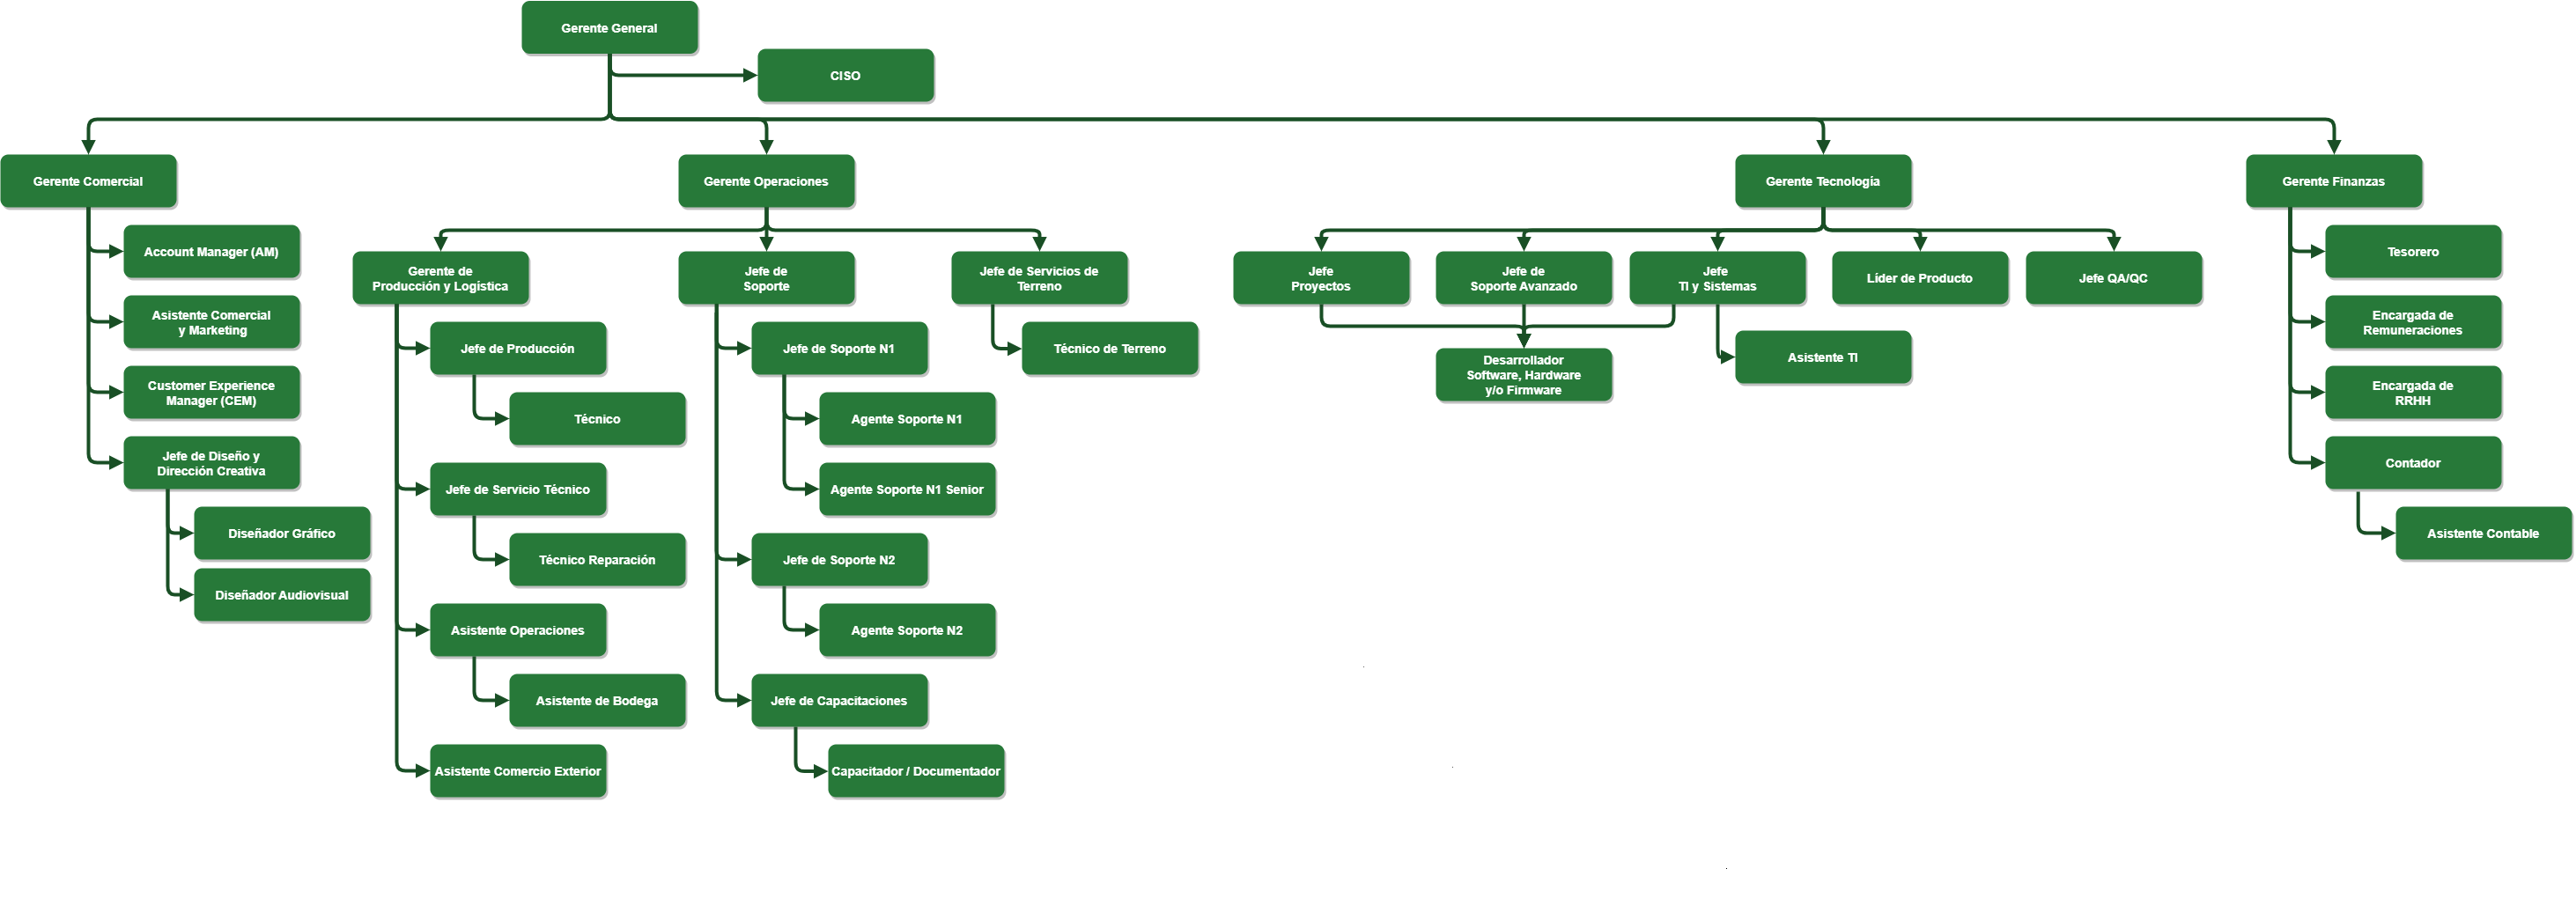
\includegraphics[width=1\textwidth]{Organigrama_WiseConn}
	\caption{\label{fig:orgwis} Organigrama de Wiseconn}
\end{figure}

\subsection{PRODUCTOS}
\subsubsection{HARDWARE}

El hardware ha sido especialmente diseñado por la empresa para el monitoreo y control de riego, los componentes principales son los nodos, dispositivos de monitoreo y control IoT que operan en terreno y se comunican mediante radio y celular para conectarse a la nube. Existen los siguientes 3 modelos, los cuales se diferencian según si se quiere realizar un simple monitoreo, control en terreno o control completo sobre los componentes de un sistema de riego.
\begin{itemize}
	\item \textbf{RF-M1:} Nodo de monitoreo de campo. Permite obtener información de variables agroclimáticas, variables de suelo, sensores de riego y variables de planta.
	\item \textbf{RF-X1:} Nodo de monitoreo y control de campo. Permite el control y monitoreo de válvulas, monitoreo de campo, control de la estación de bombeo, control de fertirriego, control PID y automatización remota.
	\item \textbf{RF-C1:} Nodo de control de caseta de riego. Permite el control y monitoreo de casetas de riego, válvulas, retrolavados e inyección de fertilizantes y pH, monitoreo y control de variadores de frecuencia y automatización industrial remota.
\end{itemize}

\subsubsection{SOFTWARE}
Wiseconn ofrece Software como Servicio o SaaS (del inglés, Software as a Service), ya que, estos se acceden mediante la web sin necesidad de instalación previa. Estos servicios ofrecen el almacenamiento y visualización de información recolectada en terreno y permiten configurar los componentes de una manera óptima y sin complicaciones. Los softwares que ofrecen son:
\begin{itemize}
    \item \textbf{DropControl:} Es una plataforma online que permite el monitoreo de control y riego/fertirriego avanzado, capaz de conectarse con cualquier sensor, equipo de riego y fertilización de manera simple y confiable.
    \item \textbf{Aplicación Móvil:} Plataforma móvil enfocada a los operadores en terreno, para el monitoreo y control de riego, monitoreo de variables, informes calicatas, notificaciones de alarmas.
    \item \textbf{Admin de DropControl:} Servicio enfocado a los usuarios administradores de campo para realizar modificaciones de sectores de riego, usuarios, servicios API, entre otros.
\end{itemize}

Para estos servicios se ofrecen planes, cuyos factores diferenciales son esencialmente herramientas especializadas, el acceso a la aplicación web y/o móvil, cantidad de usuarios permitidos, almacenamiento, acceso a funcionalidades, entre otros.
Wiseconn también tiene software interno utilizado por trabajadores de distintas áreas de la empresa como soporte y producción, para hacer configuraciones avanzadas de campos o temas productivos como manejo de inventarios, lotes, despachos, etc. Dentro de estos softwares están:
\begin{itemize}
    \item \textbf{Operations:} Plataforma para la gestión de lotes y despacho de productos.
    \item \textbf{Setup:} Plataforma de configuración paso a paso. Provee herramientas de gestión para cuentas, campos y usuarios con el fin de crear y organizar los permisos a usar en DropControl o en el mismo Setup.
\end{itemize}

\subsection{PRESENCIA EN EL MERCADO}
WiseConn esta presente a lo largo de más de 1000 campos en países como Chile, Perú y Estados Unidos. Dentro de algunos casos de éxito está:
\begin{itemize}
	\item \textbf{Fowler Packing:} Operación agrícola operada y de propiedad familiar en Fowler, California, y cultiva 12000 acres de diversos cultivos en todo el valle central sur. Fowler Packing ha estado usando Dropcontrol durante 4 años y fue una de las primeras operaciones en utilizar sus caracteristicas. Dentro de los resultados estan:
		\SubItem{Reducción del uso de agua en un 30\%: su mayor beneficio económico.}
		\SubItem{Aumento de los rendimientos en un 20\%.}
		\SubItem{Reducción de los costos de energía de PG\&E.}
	\item \textbf{Fresno State:} Proyecto con el objetivo de analizar como las necesidades de agua de los cultivos pueden variar en funcin de diferentes clasificaciones. Este proyecto específico está comparando el riego basado en los requisitos de humedad del suelo con los requisitos de ET (evapotranspiración).
	\item \textbf{Cran Chile:} Agricola Cran Chile dirigido por Victor Bascuñan, posee 7 campos ubicados entre la región de la Araucanía y la región de Los Ríos los cuales tienen 680 hectáreas de Cranberries, con monitoreo de clima y suelo a través de Dropcontrol.
	\item \textbf{Aconcagua Foods:} Cuenta con 6 campos diseñados por SCF Ingeniería, ubicados entre la comuna de Paine y San Fernando (Chile), con una superficie plantada de 506 há de cultivo de Durazno conservero, Año plantación 2000 y 2020, riego por goteo con doble línea 2 mm precipitación con control de riego DropControl, monitoreo de clima y sensores de humedad de Consultora Diestre.
\end{itemize}

\subsection{SITUACIÓN ACTUAL}

\subsubsection{DESCRIPCIÓN}
En la actualidad, el usuario cliente no tiene completo acceso para realizar ciertas configuraciones en los campos debe recurrir al área de soporte mandando un ticket con la configuración a realizar. Algunas de estas configuraciones son procesos que consumen mucho tiempo y esfuerzo para los trabajadores de soporte. Esto puede significar una carga innecesaria y/o un aumento en el personal para poder llevar a cabo estos procesos en un tiempo razonable. Por el lado del usuario cliente, genera un descontento debido a la alta espera por la configuración.
En los procesos productivos, las herramientas de softwares son limitadas y los trabajadores deben hacer pasos extras innecesarios para poder realizar la tarea correspondiente. Debido a esto, se pueden generar algunos errores y retrasos en producción.
Como se explicó anteriormente, Wiseconn ofrece planes gratuitos y de pago. En el caso del plan gratuito, este habilita un punto de entrada para aquellos usuarios que no están dispuestos a realizar pagos recurrentes. Sin embargo, existen limitaciones para el usuario cliente debido a la baja cantidad de funcionalidades y/o herramientas disponibles, lo que impide poder entregar condiciones mínimas al usuario que cumplan con las especificaciones comerciales. Además, puede influir en la poca retención de usuarios y/o que estos no se cambien a un plan de pago.

\subsubsection{ACTORES}
Dentro de los actores está, primero, el usuario cliente que utiliza y/o paga los servicios que ofrece Wiseconn para la gestión de riego de sus campos. Segundo, los trabajadores de Wiseconn del área de soporte y producción que utilizan los softwares internos para la realización de sus respectivas tareas.

\subsubsection{ÁRBOL DEL PROBLEMA}
En la figura \ref{fig:arbolproblema} se encuentra representado el árbol del problema, que identifica como problema principal las funcionalidades limitadas del software de Wiseconn y alta intervención humana en el proceso.
En la parte inferior se presentan las causas representadas en que el usuario depende del área de soporte para la realización de algunas configuraciones, el plan gratuito no cumple con las especificaciones comerciales mínimas y, por último, procesos que consumen mucho tiempo y esfuerzo para los trabajadores.
En la parte superior, se presentan los efectos que puede generar este problema como el aumento en la posibilidad de errores, retrasos en producción, usuario final descontento por la espera de las configuraciones, el usuario no cambia al plan de pago o cancela sus servicios y mayor carga en el área de soporte.

\begin{figure}
    \centering
	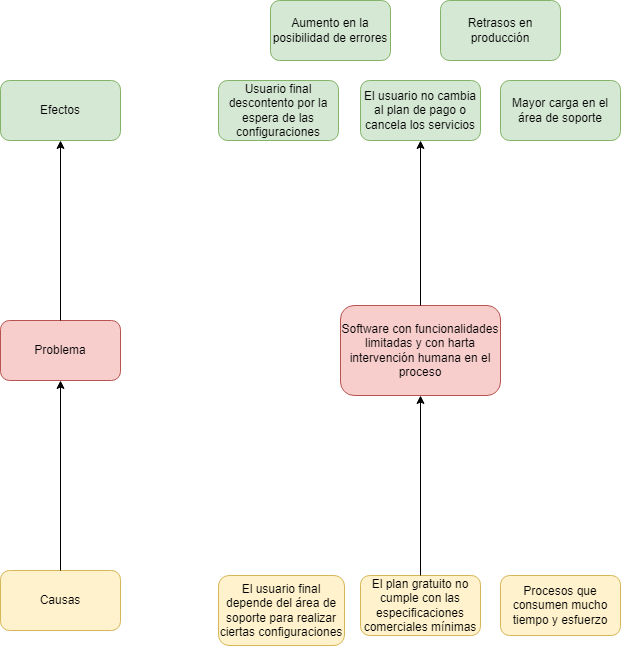
\includegraphics[width=0.8\textwidth]{arbol del problema}
	\caption{\label{fig:arbolproblema} Árbol del problema} Fuente: Elaboración propia.
\end{figure}

\subsection{SOLUCIÓN}

\subsubsection{OBJETIVO GENERAL}

Análisis, diseño e implementación de herramientas de software que faciliten tareas a usuarios y mejoren procesos para un escalamiento global de servicios de WiseConn, para así, poder reducir tiempo y esfuerzo en los trabajadores de distintas áreas de la empresa, como también, reducir la brecha asociadas a los cobros de servicios SaaS.

\subsubsection{OBJETIVOS ESPECÍFICOS}
\begin{itemize}
    \item Realizar un análisis de los procesos de producción que más cargan y esfuerzo generan, como también de funcionalidades/herramientas necesarias para el plan gratuito.
    \item A partir del análisis previo, diseñar las herramientas de software correspondientes para los servicios de WiseConn.
    \item Implementación de las herramientas de software en los servicios de WiseConn correspondientes.
\end{itemize}

\subsubsection{ALCANCE DE LA SOLUCIÓN}
Al finalizar esta memoria se espera reducir los tiempos y esfuerzos en las áreas de soporte y producción de la empresa, ya sea, mejorando herramientas internas o transfiriendo tareas/procesos al usuario cliente. También, ayudar a reducir la brecha de cobros en servicios SaaS con alternativas gratuitas de ciertas funcionalidades, lo que permitiría que el plan gratuito de Wiseconn cumpla con las especificaciones comerciales.

\newpage
\secnumbersection{MARCO CONCEPTUAL}

\subsection{CONCEPTOS TÉCNICOS}

\subsubsection{\textit{SOFTWARE AS A SERVICE (SaaS)}} 

El software como servicio o SaaS (Software as a Service, en inglés) es un tipo de servicio de cloud computing que se enfoca en la entrega de software basado en la nube, para esto se necesita un proveedor de servicios de nube que desarrolla y mantiene el software de las aplicaciones, proporciona actualizaciones automáticas y lo pone a disposición de sus clientes a través de Internet con un sistema de pago por uso. De este modo, los clientes del SaaS reducen sus costos.\footnote{\href{https://www.oracle.com/applications/what-is-saas/}{Oracle - What is SaaS?}}

\subsubsection{\textit{WEB FRAMEWORKS}}

En los inicios del desarrollo web todas las aplicaciones eran programadas “a mano”, lo que provocaba muchos errores. Para poder superar estas dificultades se introdujeron los Web Frameworks en los inicios de la década de los 2000. Los webs frameworks son herramientas que ayudan a construir un sitio web disminuyendo bugs, errores y tiempo. Los frameworks se dividen principalmente en dos categorías: Front-end y Back-end. \cite{analysiswf} 

\subsubsubsection{\textit{FRONT-END}}

También conocido como \textit{client-side}, es el componente de la aplicación o página web con el que el usuario interactúa. Incluye lo que el usuario ve como imágenes, botones, colores, gráficos, tablas, entre otros. HTML y CSS son usados para el diseño y estilo, mientras que JavaScript se utiliza para validaciones, animaciones, cambios de estado, etc. El rendimiento y la sensibilidad son los 2 grandes objetivos del desarrollo front-end. El desarrollador se asegura que la aplicación sea sensible, es decir, que se muestren las vistas correctamente en diferentes pantallas como las de monitor, celular, tablets. \cite{webframedbws}

\subsubsubsection{\textit{BACK-END}}

En \textit{back-end} las preocupaciones son otras, por ejemplo, protección de APIs de ataques externos, autenticar usuarios, interacción con bases de datos y manejar solicitudes de usuarios. Los frameworks de back-end son evaluados según sus métodos de programación, lenguajes que soporta e interfaces. También, proveen herramientas y plantillas que ayudan a los desarrolladores en varias tareas del desarrollo. \cite{webframedbws}

\subsubsection{\textit{APPLICATION PROGRAMING INTERFACE (API)}}

\textit{Application Programming Interface} (API) es un conjunto de herramientas, definiciones y protocolos que se utiliza para que los productos y servicios se comuniquen con otros, sin tener que diseñar permanentemente una infraestructura de conectividad nueva. Las API pueden ser privadas (para uso interno), compartidas (con terceros para brindar flujos de ingresos adicionales) o públicas (entidades externas pueden desarrollar aplicaciones que interactúen con sus API para fomentar la innovación).
El propósito de las API es la integración, es decir, se encargan de conectar los datos, las aplicaciones y los dispositivos para que todas las tecnologías puedan comunicarse y trabajar mejor en conjunto.

\subsubsubsection{API REST}

REST es una sigla que significa \textit{REpresentational State Transfer}, es un término acuñado por Roy Fielding presentado en su tesis doctoral \cite{fieldingapi}, y lo define como un estilo de arquitectura para sistemas distribuidos de hipermedia, describiendo las restricciones de ingeniería de software que guían REST. Estas restricciones son las siguientes:
\begin{itemize}
    \item \textbf{Arquitectura cliente-servidor:} La separación de responsabilidades es el principio detrás de esta restricción. Cuanto menos conoce el servidor del cliente, y viceversa, resulta más fácil el cambio de componentes.
    \item \textbf{Ausencia de estado:} La comunicación debe ser sin estado por naturaleza, es decir, cada petición del cliente al servidor debe contener solo la información necesaria para entender la petición y no puede tomar ventaja de ningún contexto almacenado en el servidor. Por esto, las sesiones se deben mantener en el cliente.
    \item \textbf{Caché:} La data de una respuesta a una petición debe estar implícita o explícitamente etiquetada como cacheable o no cacheable. Si la respuesta es cacheable, se pueden enviar respuestas cacheadas desde cualquier punto de la red sin necesidad que la petición llegue al servidor.
    \item \textbf{Sistema por capas:} Tiene relación con la separación de responsabilidades y establece que un cliente debe conocer únicamente la capa a la que le está hablando.  Es decir, no debe saber qué bases de datos se está utilizando, cachés, proxies, etc.
    \item \textbf{Interfaz uniforme:} La principal característica que distingue la arquitectura REST de otras es el énfasis de una interfaz uniforme entre componentes, para que la información se transfiera de forma estandarizada. 
    \item \textbf{Código bajo demanda:} REST permite extender la funcionabilidad del cliente mediante la descarga y ejecución de código en forma de scripts. 
\end{itemize}
REST es un estilo de arquitectura no un estándar, es por esto, que las API REST suelen llamarse API RESTful, es decir, una API que sigue la arquitectura REST. Puede resultar complejo implementar todos los principios de REST en una API, por ello, el modelo de madurez de Richardson (Fowler, 2010) describe cuánto se apega un servicio a las características de REST. Posee cuatro niveles:
\begin{itemize}
    \item \textbf{Nivel 0:} El servicio cuenta con una sola URI que acepta todo el rango de operaciones, con unos recursos poco definidos.
    \item \textbf{Nivel 1:} El servicio cuenta con varias URIs para distintos recursos. Necesita saber qué tipo de operación realizar a través de la URI o el payload.
    \item \textbf{Nivel 2:} El servicio hace uso de las URIs para recursos identificando la operación a través de los métodos HTTP. Además, hace un correcto uso de los códigos de estado.
    \item \textbf{Nivel 3:} El servicio implementa Hypermedia as the engine of application state (HATEOAS).
\end{itemize}
Los servicios que alcancen el nivel 3 podrán ser considerados como API RESTful.

\subsection{HERRAMIENTAS TECNOLÓGICAS}

\subsubsection{\textit{AMAZON WEB SERVICES (AWS)} }

Amazon Web Services\footnote{\href{https://aws.amazon.com/es/what-is-aws/}{¿Qué es AWS?}}, o AWS, es la plataforma en la nube más utilizada en el mundo, que cuenta con una cantidad de servicios y características ofreciendo desde tecnologías de infraestructura como cómputo, almacenamiento y bases de datos hasta tecnologías emergentes como aprendizaje automático e inteligencia artificial, data lakes e Internet of Things. Dentro de los servicios más importantes están:
\begin{itemize}
    \item \textbf{EC2:} \textit{Amazon Elastic Compute Cloud} ofrece capacidad de computación con más de 500 instancias y la posibilidad de elegir procesador, almacenamiento, redes, sistema operativo y modelo de compra para ajustar a las necesidades del usuario.
    \item \textbf{S3:} \textit{Amazon Simple Storage Service} es un servicio de almacenamiento de objetos que ofrece escalabilidad, disponibilidad de datos y un gran rendimiento. Dado que posee clases de almacenamiento y características de administración fáciles de usar, es posible optimizar costos, organizar datos y configurar controles de acceso.
    \item \textbf{RDS:} \textit{Amazon Relational Database Service} es una colección de servicios que facilita las tareas de configuración, operación y escalamiento de una base de datos en la nube. Se puede elegir entre motores como Amazon Aurora, MySQL, PostgreSQL, MariaDB, SQL Server, entre otros.
    \item \textbf{Lambda:} Servicio informático sin servidor (serverless) y basado en eventos que permite ejecutar código para cualquier tipo de aplicación o servicio back-end sin la necesidad de servidores.
\end{itemize}

\subsubsection{\textit{JAVASCRIPT}}

JavaScript, o JS, es un lenguaje de programación orientado a objetos, utilizado mayormente para el desarrollo web en ambos \textit{front-end} y \textit{back-end}. JS tiene una gran comunidad, contiene un conjunto de bibliotecas de código abierto que facilitan tareas para el desarrollador como la visualización de datos y comunicación con el usuario.

\subsubsubsection{\textit{NODE.JS}}

Node.js es un entorno en tiempo de ejecución asíncrono basado en eventos diseñada para desarrollar, mayormente, en server-side. Soporta el manejo de muchas conexiones al mismo tiempo. Node.js tiene propiedades que lo hacen escalable. Usa el motor V8 de Google para ejecutar código de JavaScript transformándolo en código máquina y optimiza mediante métodos complejos. \cite{webframedbws}

\subsubsubsection{\textit{REACTJS}}

ReactJS es una biblioteca de JavaScript para el desarrollo de interfaces de usuarios dinámicas. Creado y mantenido por Facebook. Interfaces complejas pueden ser compuestas de piezas pequeñas, asiladas y reusables de código llamadas “componentes”. ReactJS usa JSX, preprocesador que agrega sintaxis XML a JavaScript, para la escritura simple de HTML. \cite{webframedbws}

\subsubsection{\textit{JAVA}}

Java\footnote{\href{https://www.ibm.com/cloud/learn/java-explained}{What is Java? | IBM}} es un lenguaje de programación orientado a objetos lanzado en el año 1995 por Sun Microsystems. Una de las mayores ventajas del desarrollo con Java es su portabilidad, independiente en que dispositivo se programe Java se puede correr en otros dispositivos.
Java es una tecnología que consiste en el lenguaje de programación y una plataforma de software. Para crear aplicaciones con Java se necesita descargar el Java Development kit (JDK). Se escribe el código, luego un compilador lo transforma a Java bytecode que corre en la Java Virtual Machine (JVM). Cualquier sistema que soporte JVMs puede correr aplicaciones Java.

\subsubsubsection{\textit{JAVASERVER FACES}}

JavaServer Faces\footnote{\href{https://www.juntadeandalucia.es/servicios/madeja/contenido/recurso/101}{JavaServer Faces (JSF)}} (JSF) es una infraestructura de interfaz de usuario o de APIs que facilita el desarrollo de aplicaciones web de Java. JSF usa principalmente JavaServer Pages (JSP) para el despliegue de las páginas. Los principales componentes son:
\begin{itemize}
    \item Una API para representar componentes de interfaz de usuario y gestionar su estado.
    \item Dos bibliotecas de etiquetas JSP para expresar componentes en una página JSP y enlazar los componentes a objetos del servidor.
\end{itemize}
Una de las grandes ventajas de JSF es la clara separación entre el comportamiento y la presentación, esto permite que cada desarrollador de un equipo se enfoque en su parte del proceso de desarrollo, y proporciona un modelo de programación sencillo para enlazar las piezas. No obstante, en comparación con otros entornos o arquitecturas, no es muy rápida.

\subsection{ESTADO DEL ARTE}
La tecnología de WiseConn permite a los administradores de campo poder monitorear, controlar y automatizar de manera inalámbrica los sistemas de riego para aumentar los ingresos, disminuir los gastos y ayudar a administrar el tiempo.

En terreno, una red de nodos inteligentes se conectan a sensores y actuadores recopilando información de clima, humedad de suelo, riego, nutrición, entre otros. Estos nodos se comunican entre si por medio de señales de radio enviando la información a la nube, donde es almacenada y gestionada por servidores en \textit{Amazon Web Services}. Los datos se despliegan en Dropcontrol para su análisis en tiempo real, simplificando las tareas de riego reduciendo costos de mano de obra, agua y energía.
\begin{figure}[H]
	\centering
	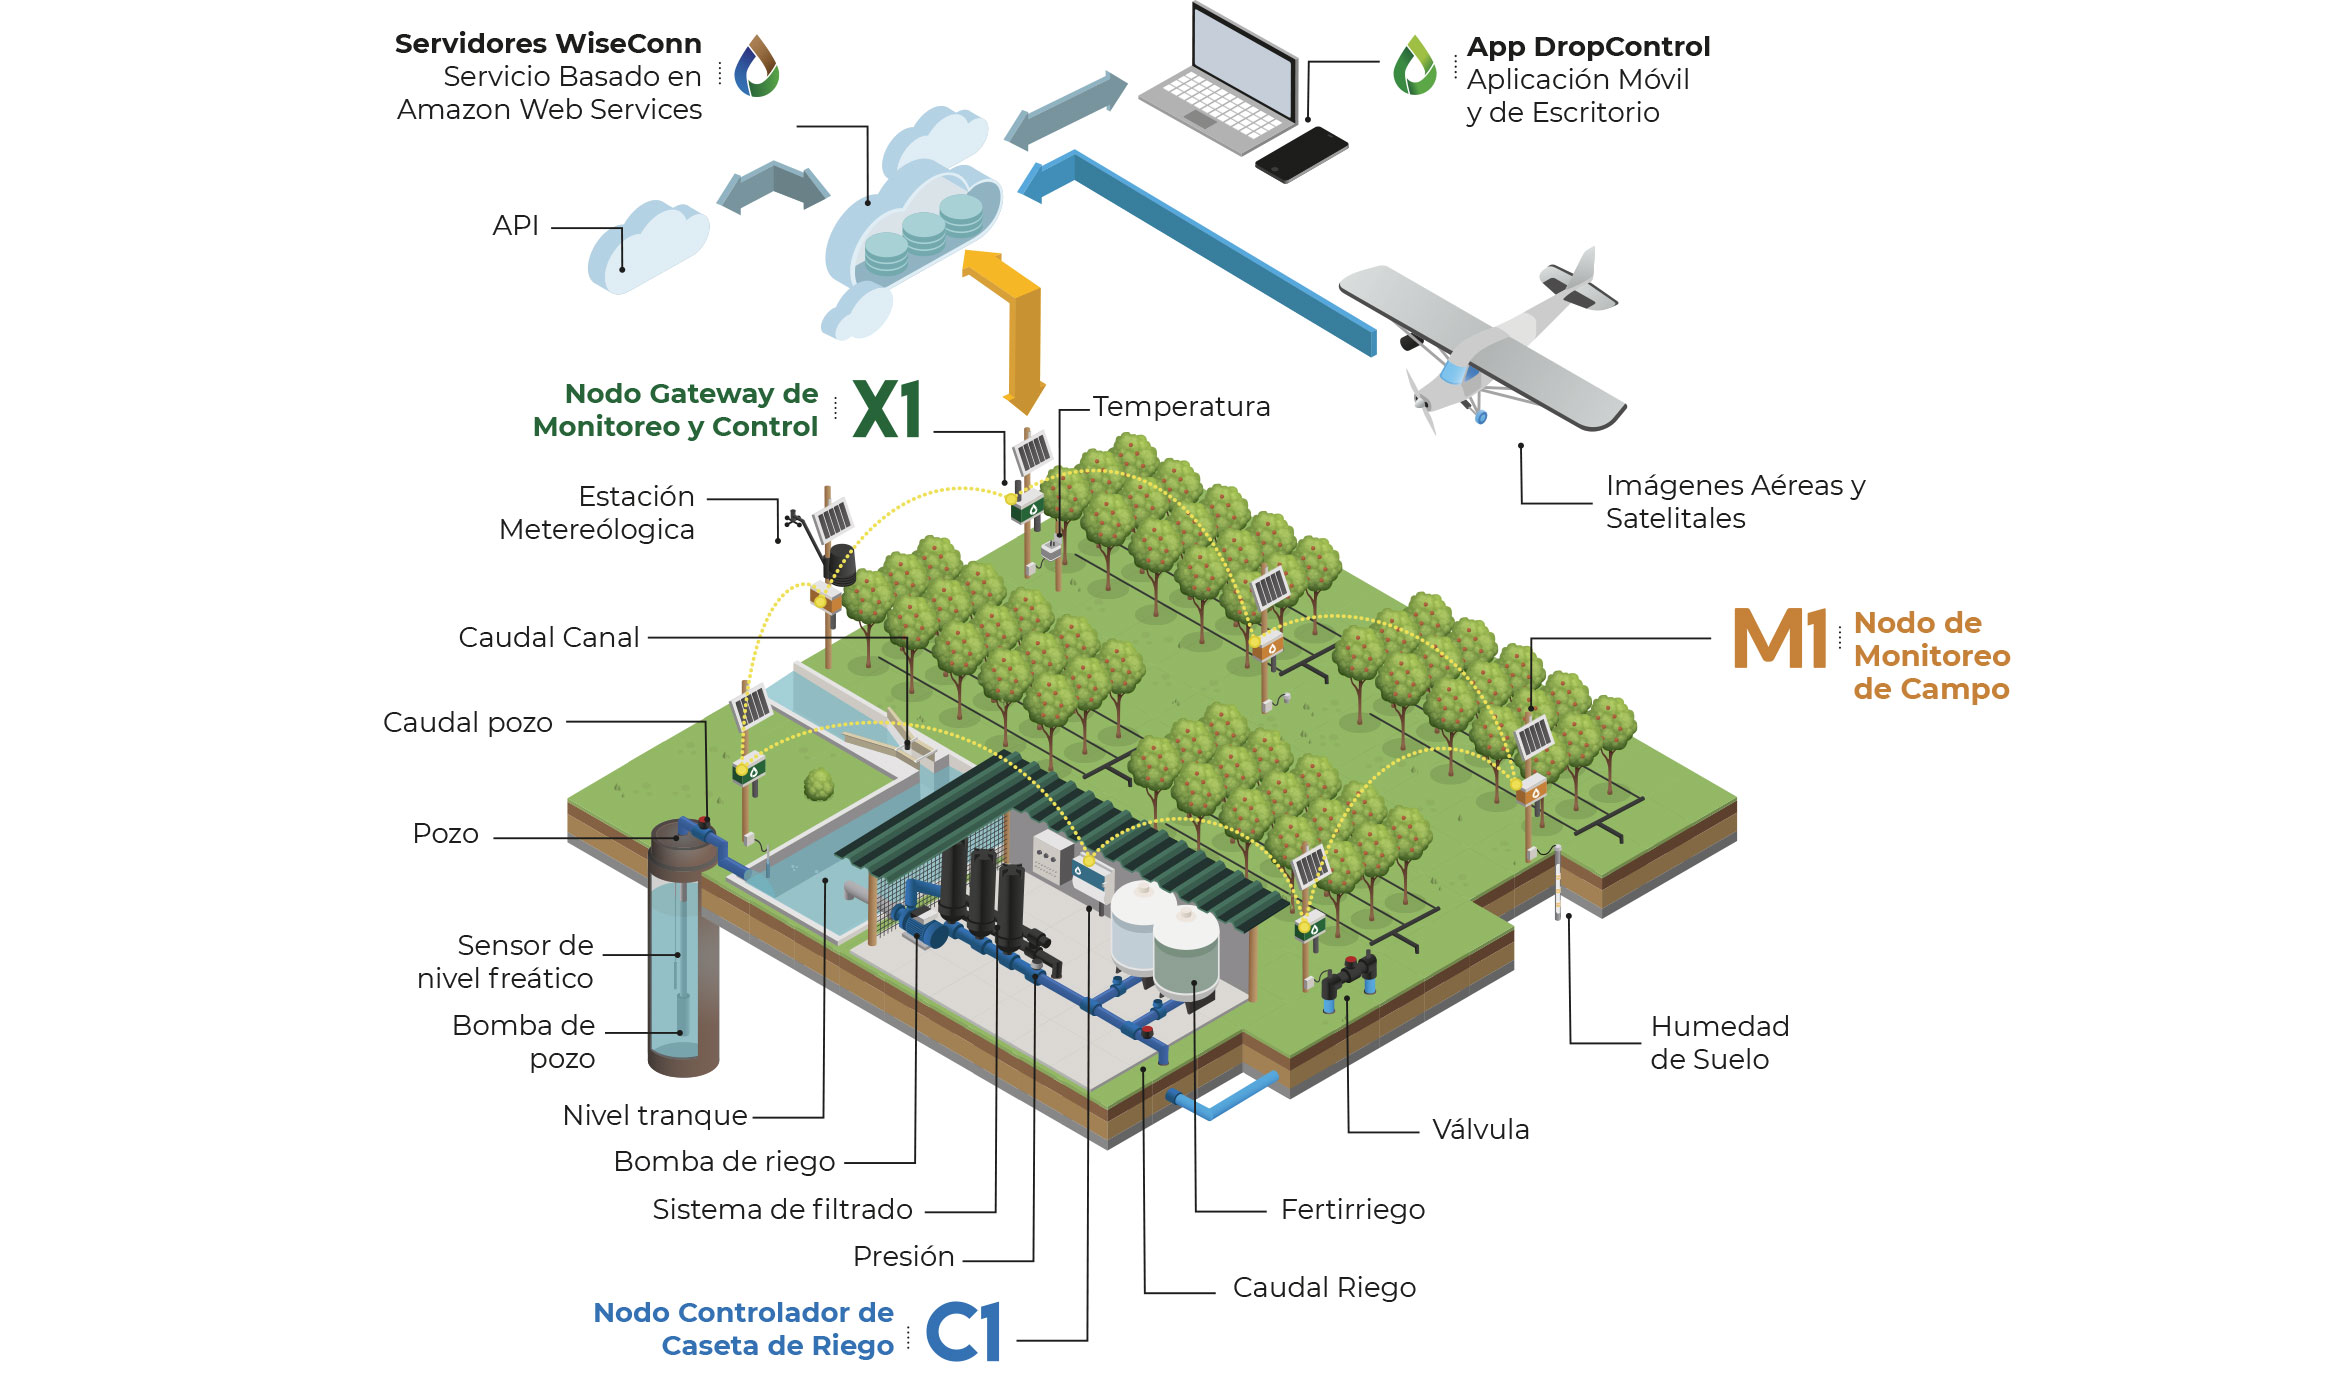
\includegraphics[width=1\textwidth]{mundo_dropcontrol}
	\caption{\label{fig:mundrop} ¿Cómo funciona DropControl?}
\end{figure}

\subsubsection{COMPETENCIAS EN EL MERCADO}

\subsubsubsection{NETAFIM}
NETAFIM\footnote{\href{https://www.netafim.com/en/}{NETAFIM}} es una empresa que provee soluciones de riego para la agricultura sustentable a nivel global, con presencia en más de 110 países.
Dentro de los productos y soluciones que ofrece para el riego de presición están:
\begin{itemize}
    \item \textbf{Goteros y líneas de goteo} 
    \item \textbf{Aspersores, microaspersores y emisores especiales}
    \item \textbf{Filtros}
    \item \textbf{Válvulas}
    \item \textbf{Tubería Flexible y Tubos de PE}
    \item \textbf{Conectores}        
\end{itemize}
NETAFIM también ofrece \textit{Digital Farming} que permite un manejo más inteligente, rápido y preciso en la irrigación. Está compuesto de tres familias de productos: Sistemas de monitoreo y manejo de cultivos, controladores y sistemas de dosificación.
Teniendo en cuenta todas las condiciones de suelo, clima, cultivo, medio ambiente y las condiciones hidráulicas, las soluciones alojadas en la nube presentan una imagen de la situación del campo en tiempo real y datos a los que puede acceder el productor a través del computador o dispositivo móvil. Esto permite a los agricultores administrar, controlar y optimizar el riego y la fertirrigación de acuerdo a las necesidades del cultivo.

Dentro del \textit{Digital Farming} está \textit{GrowSphere}\footnote{\href{https://www.netafim.com/en/digital-farming/}{\textit{GrowSphere}}}, que es el primer sistema operativo para el riego preciso (figura \ref{fig:netafim}). Una herramienta simple, intituiva y visual que ayuda a planear y ejecutar los planes de riego.
\begin{figure}[H]
	\centering
	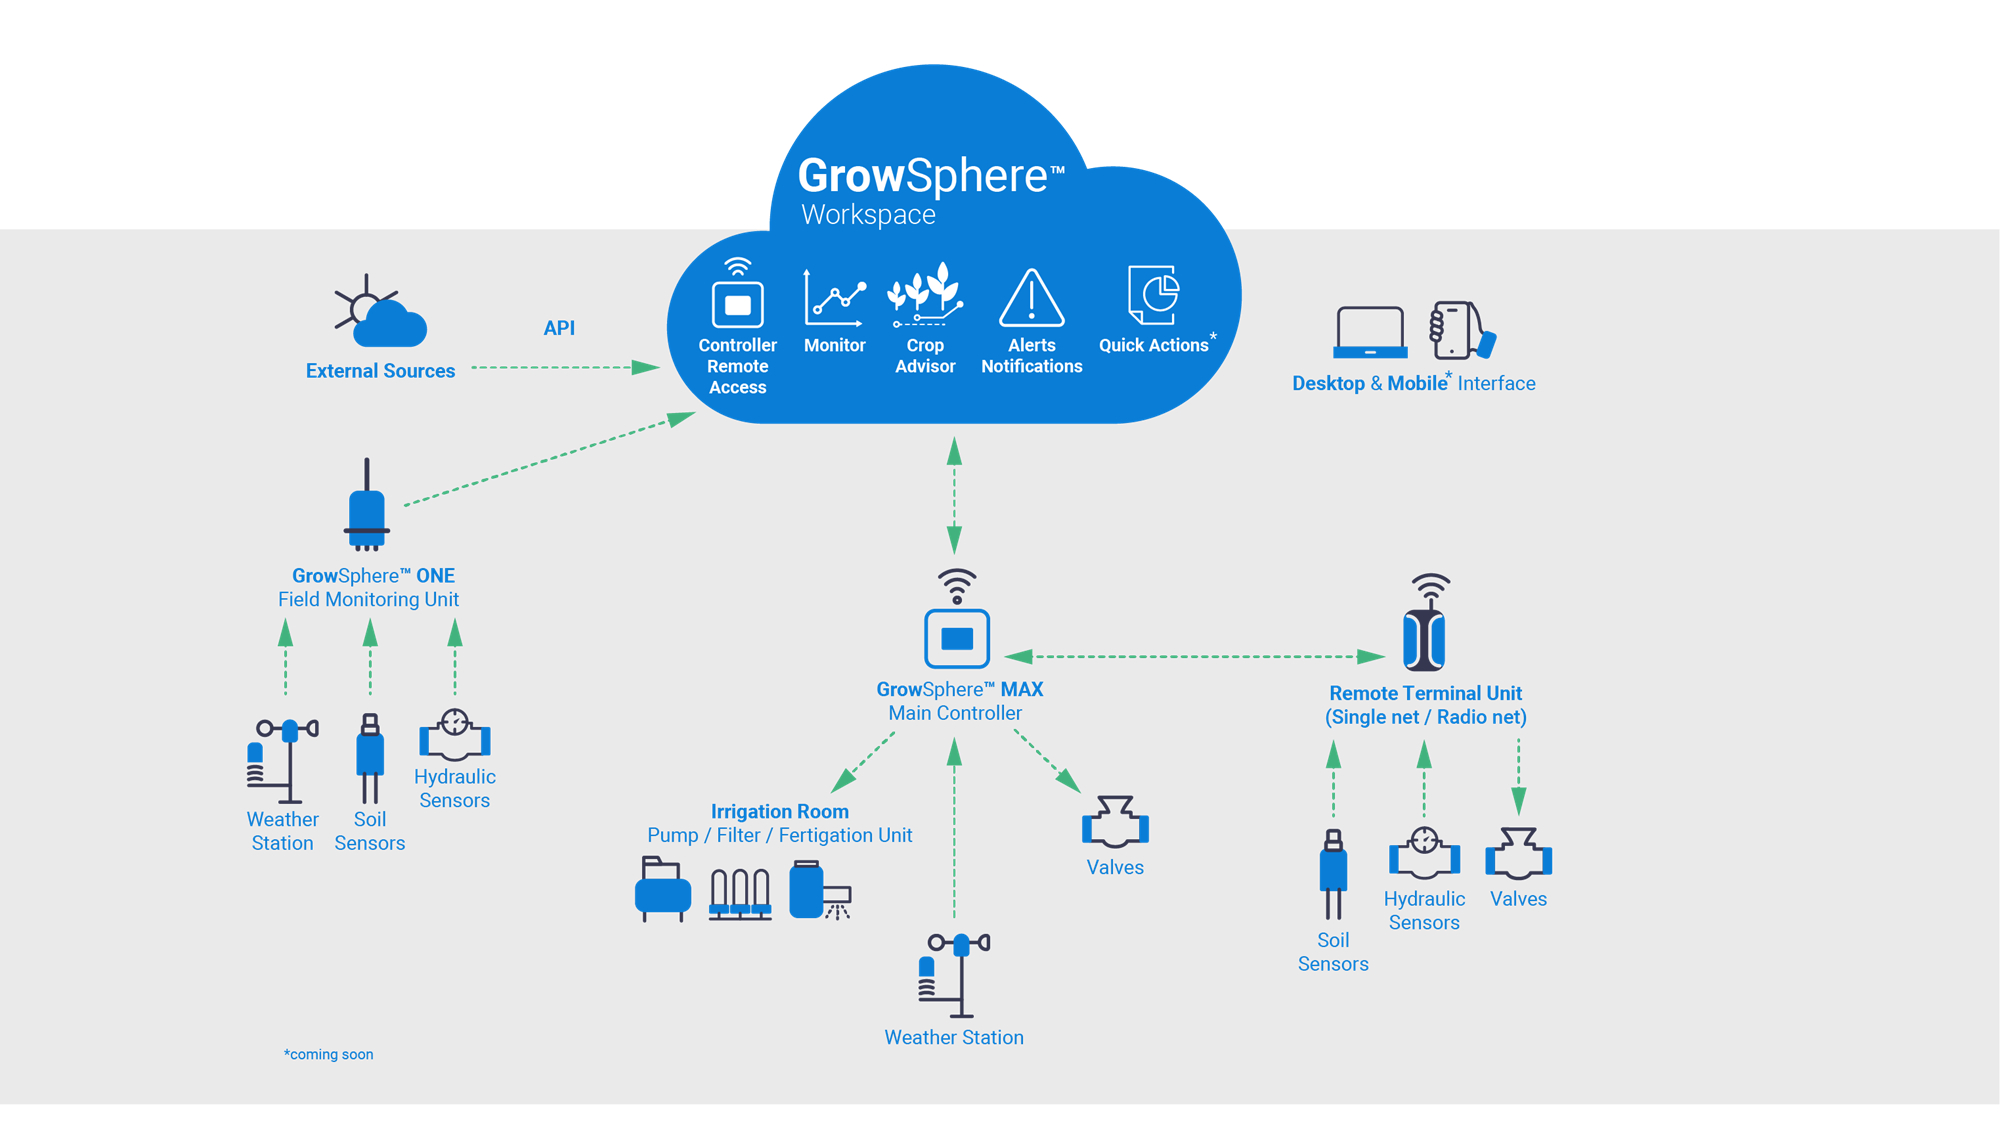
\includegraphics[width=1\textwidth]{netafim}
	\caption{\label{fig:netafim} \textit{Digital Farming}}
\end{figure}

NETAFIM tiene 3 planes de servicio:
\begin{itemize}
    \item \textbf{\textit{Irrigation as a Service (IaaS)}:} El sistema de riego es operado, mantenido y de propiedad de NETAFIM. 
    \item \textbf{Operación y Mantenimiento:} NETAFIM opera y mantiene los sistemas de propiedad del usuario cliente.
    \item \textbf{Servicio Anual:} Un programa de soporte agronómico y técnico de los expertos de NETAFIM. Diagnostican las mejoras y el mantenimiento del sistema de riego, que es operado por el agricultor y de su propiedad.
\end{itemize}

\subsubsubsection{HORTAU}
HORTAU\footnote{\href{https://hortau.com/es/}{HORTAU}} proporciona a los productores información en tiempo real sobre las condiciones del suelo y el clima para ayudarles a tomar decisiones informadas sobre el riego y la fertilización.
Utiliza sondas de tensión matricial del suelo que envían información a una aplicación móvil, permitiendo al usuario monitorear el movimiento del agua y los nutrientes en todo perfil del suelo y determinar el momento y la cantidad adecuada de riego (figura \ref{fig:hortau}).
HORTAU cuenta con más de 1300 granjas, 7000 estaciones y 20 años de experiencia en el rubro.

Dentro de los servicios que ofrece HORTAU están:
\begin{itemize}
    \item \textbf{Manejo de riego.}
    \item \textbf{Programación y asesoramiento.}
    \item \textbf{Automatización del riego.}
    \item \textbf{Monitoreo de caudalímetros.}
    \item \textbf{Monitoreo de profundidad de pozo.}
    \item \textbf{Monitoreo de clima.}
\end{itemize}

\begin{figure}[H]
	\centering
	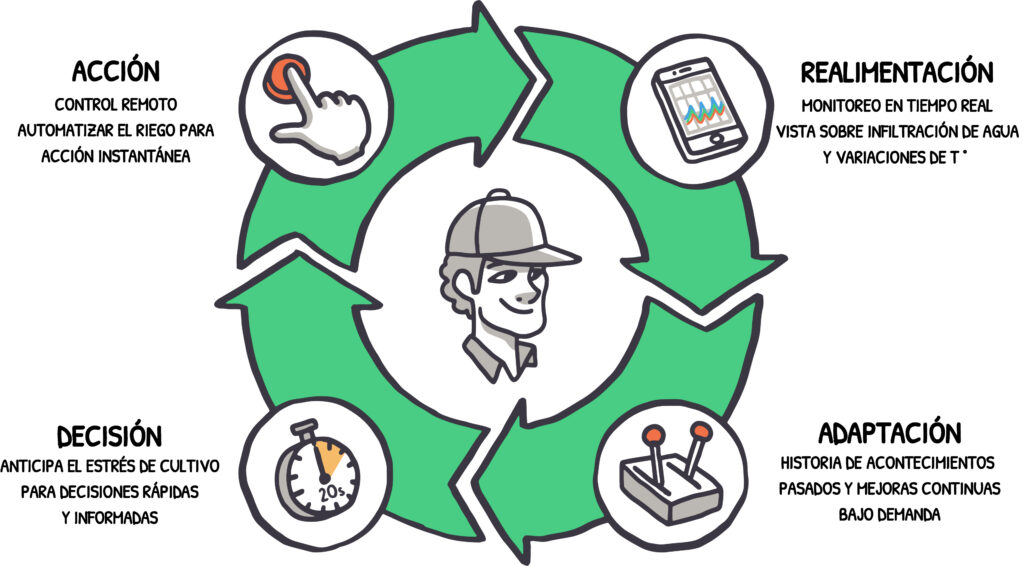
\includegraphics[width=1\textwidth]{hortau}
	\caption{\label{fig:hortau} \textit{Hortau}}
\end{figure}

\subsubsubsection{MOTTECH}
Mottech Water Solutions Ltd.\footnote{\href{https://mottech.com/}{Mottech Water Solutions Ltd.}} es un distribuidor de \textit{Motorola solutions}. Mottech ofrece soluciones de monitoreo y control remoto para diversos mercados y aplicaciones, incluyendo riego agrícola, riego de césped y paisajismo, y distribución de agua.

Dentro del mercado del riego agrícola ofrece una robusta y confiable solución, que incluye riego agrícola y su monitoreo y control, logrando un riego preciso y profesional que al mismo tiempo ahorra energía, mano de obra, costos de fertilizantes y agua.

Mottech ofrece los siguientes productos y servicios:
\begin{itemize}
    \item \textbf{\textit{Irrigation Control System (IRRInet)}:} Sistema basado en una infraestructura de comunicaciones robusta y eficiente que ofrece conectividad con las válvulas y sensores para un completo control.
    \item \textbf{\textit{Management \& Control}:} \textit{ICC PRO} server software y aplicación móvil que permite un acceso seguro para el manejo y control del agua en tiempo real.
    \item \textbf{\textit{Controllers}:} Un catálogo de unidades de campo que cumplen con las necesidades de cualquier proyecto del cliente, incluyendo sitios sin servicio eléctrico.
    \item \textbf{Productos complementarios:} Completa integración con el sistema \textit{IRRInet} para incrementar la funcionalidad. Dentro de los productos están: \textit{Smart card} para expandir la compatibilidad del sensor, estación de clima integrado para el cambio automático de riego según las condiciones climáticas y, por último, una máquina de fertirriego para aplicaciones costo-efectivas. 
\end{itemize}
\newpage
\secnumbersection{PROPUESTA DE SOLUCIÓN}


\subsection{DISEÑO DE LAS SOLUCIÓN}

Entendiendo los problemas de los productos de software quue ofrece la empresa y las consecuencias que esto conlleva,
se plantean nuevas herramientas de software y/o mejoras a herramientas existentes que ayuden a liberar carga y esfuerzo
de ciertos procesos a las áreas de soporte y producción, además, darle al usuario cliente nuevas herramientas para que tenga un mejor flujo de trabajo.
Las nuevas funcionalidades serán implementadas en 3 productos de WiseConn: \textit{Admin} de DropControl, \textit{Operations} y \textit{Setup}.

\subsubsection{ADMIN DE DROPCONTROL}

Esta aplicación surge de la necesidad de los administradores de campos de poder gestionar los distintos elementos de los campos como los sectores, red de nodos, mapa, etc. de una manera rápida y sencilla.
Dentro de la aplicación se puede hacer:

\begin{itemize}
    \item Visualizar en mapa los campos de la cuenta.
    \item Revisar las relaciones del campo como los dispositivos (nodos), sensores, hidráulicas, entre otros.
    \item Parámetros comerciales.
    \item Edición de parámetros de sectores.
    \item Informaciones de equipos de riego.
    \item Asociar usuarios al campo.
    \item Visualizar APIs de terceros e integradores.
\end{itemize}

\subsubsubsection{CONFIGURADOR DE MAPA}

En la aplicación \textit{DropControl}, el usuario tiene a su disposición el mapa de su campo en el cual puede visualizar sus sectores y nodos instalados (Figura \ref{fig:mapa-dropcontrol}).
\begin{figure}[H]
	\centering
	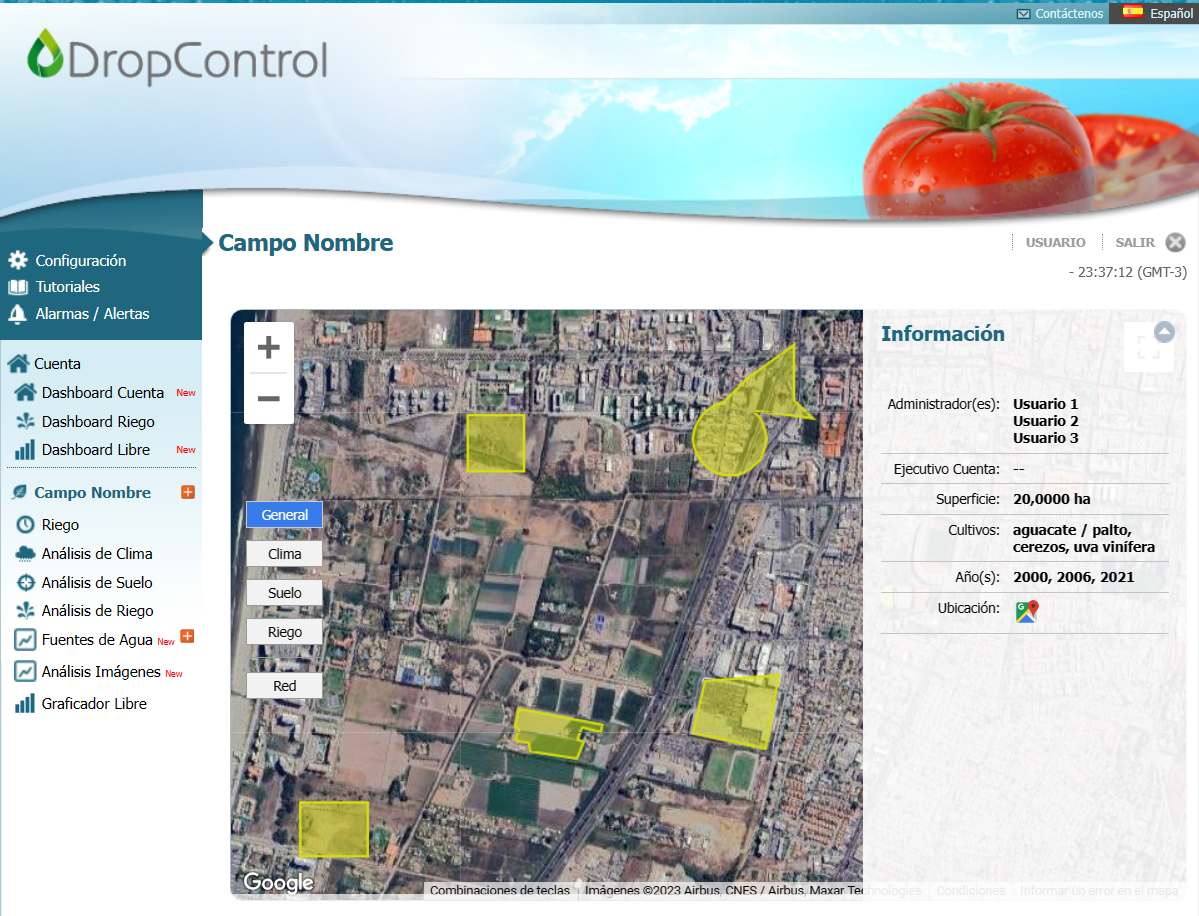
\includegraphics[width=0.8\textwidth]{mapa-dropcontrol}
	\caption{\label{fig:mapa-dropcontrol} \textit{Dashboard} de Campo - DropControl}
\end{figure}

Para mostrar el mapa se utiliza la api de \textit{Google Maps} y se utilizan los polígonos para marcar los sectores del campo y los puntos para los nodos.
Para poder configurar este mapa se puede hacer de dos maneras:
\begin{enumerate}
    \item En la aplicación \textit{Admin de DropControl}, ingresar de manera individual a cada sector/nodo y agregar su respectivo polígono/punto de manera individual.
    \item Enviar un ticket al área de soporte con un archivo con formato .kmz o .kml que contiene los polígonos y/o puntos para sus respectivos sectores y/o nodos.
\end{enumerate}
Para la primera opción, si el campo tiene demasiados sectores/nodos conllevará mucho tiempo en asginar los polígonos/puntos respectivos.
En la segunda opción existen problemas como el tiempo que demora el área tome el ticket y realize la confgiruación y/o
que las instrucciones no están bien indicadas llevando a que esta configuración requiera varios tickets para que se haga como el usuario cliente quiera.

Es por esto que se plantea una herramienta en la aplicación de \textit{Admin de DropControl} para que el usuario cliente sea el que
configure el mapa, subiendo su archivo .kmz o .kml y asignando los polígonos/puntos a sus respectivos sectores/nodos.
Junto con esto, tambien se agrega la funcionalidad de poder descargar el mapa de su campo en formato .kmz.

Esta nueva herramienta se encontrará en la vista del campo, en el mapa del campo se encontrarán dos botones (en la posisción que muestra la figura \ref{fig:mapcfg-farm}): Un botón para la descarga del mapa en formato .kmz y otro botón para poder entrar al configurador de mapa.

\begin{figure}[H]
	\centering
	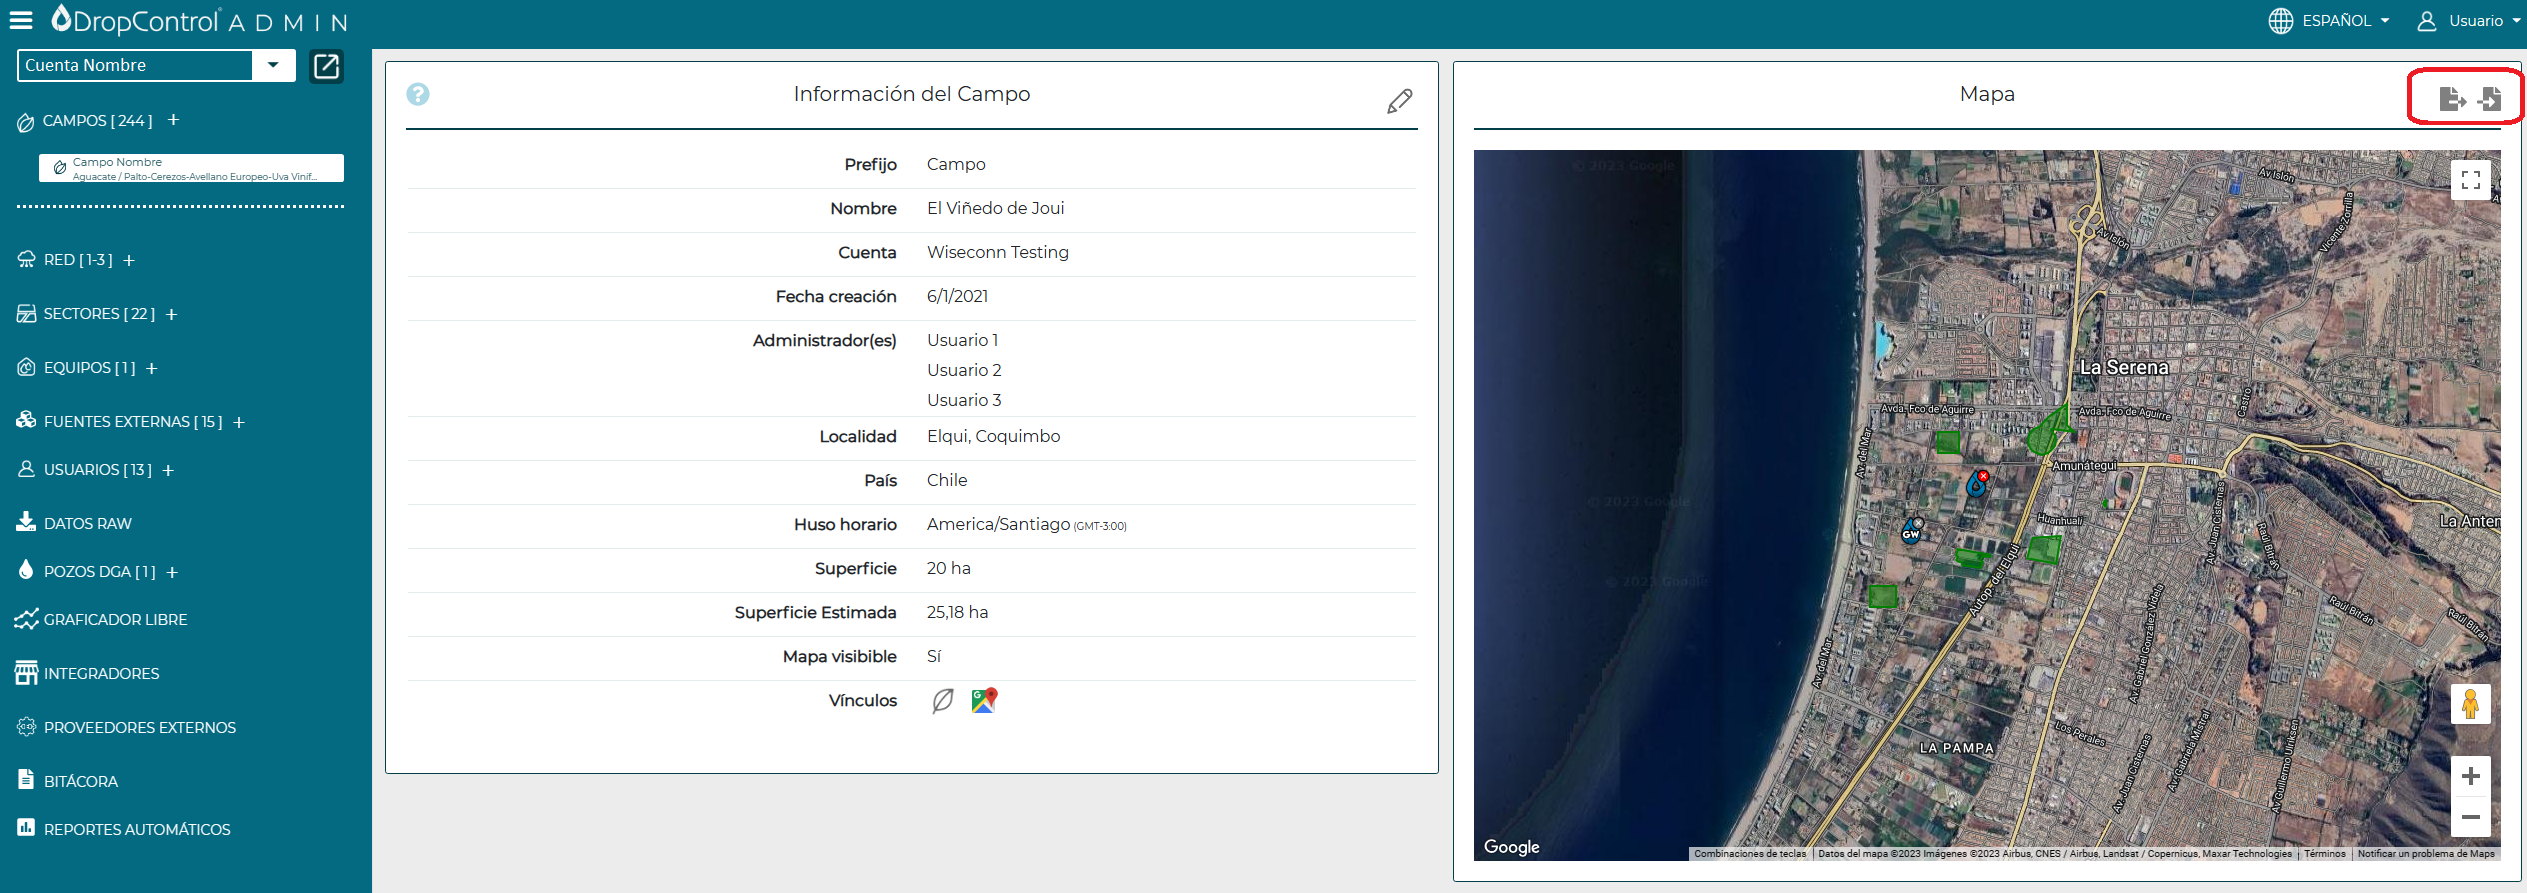
\includegraphics[width=0.8\textwidth]{mapcfg-farm}
	\caption{\label{fig:mapcfg-farm} Posición de botones de descarga de mapa y configurador de mapa.}
\end{figure}

Al hacer click en el botón de descarga del mapa, se descargará, valga la redundancia, el mapa del campo en un archivo con formato .kmz. El usuario descargando el mapa, le permite poder hacer cambios en ese archivo en aplicaciones que permitan la extensión .kmz (ejemplo, Google Earth) y después cargarlo en el configurador de mapa y actualizar sus sectores y/o nodos en el mapa del campo.

Al entrar en el configurador de mapa esta vista se divide en 2 secciones (Figura \ref{fig:mapcfg-esquema}): Tabla de sectores/nodos y el mapa.
\begin{figure}[H]
	\centering
	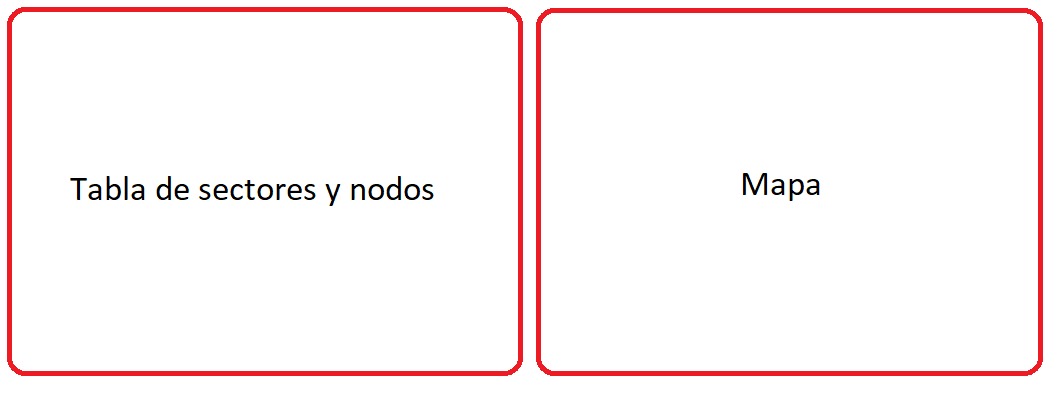
\includegraphics[width=0.8\textwidth]{mapcfg-esquema}
	\caption{\label{fig:mapcfg-esquema} Esquema de configurador de mapa. Fuente: Elaboración propia.}
\end{figure}

En la tabla de sectores/nodos (Figura \ref{fig:mapcfg-tables-exameple}) se compone de:

\begin{itemize}
    \item \textbf{Botones:}
          \begin{itemize}
              \item En la parte superior izquierda estan los botónes para cambiar entre la tabla de sectores y nodos.
              \item En el lado opuesto, se encuentra el botón de "Cargar Archivo" que, como indica el nombre, es para poder subir el archivo .kmz o .kml que contiene los polígonos y puntos para asignar.
          \end{itemize}
    \item Tabla:  
    \begin{itemize}
        \item La tabla muestra los sectores o nodos, según lo seleccionado.
        \item En primera instancia contiene dos columnas, la primera con el nombre del sector/nodo y la segunda es una columnna de acciones, con un botón que sirve para centrar el sector/nodo en el mapa. 
        \item Además, la tabla es paginada permitiendo al usuario elegir cuantos elementos mostrar por página.
    \end{itemize}
\end{itemize}

\begin{figure}[H]
	\centering
	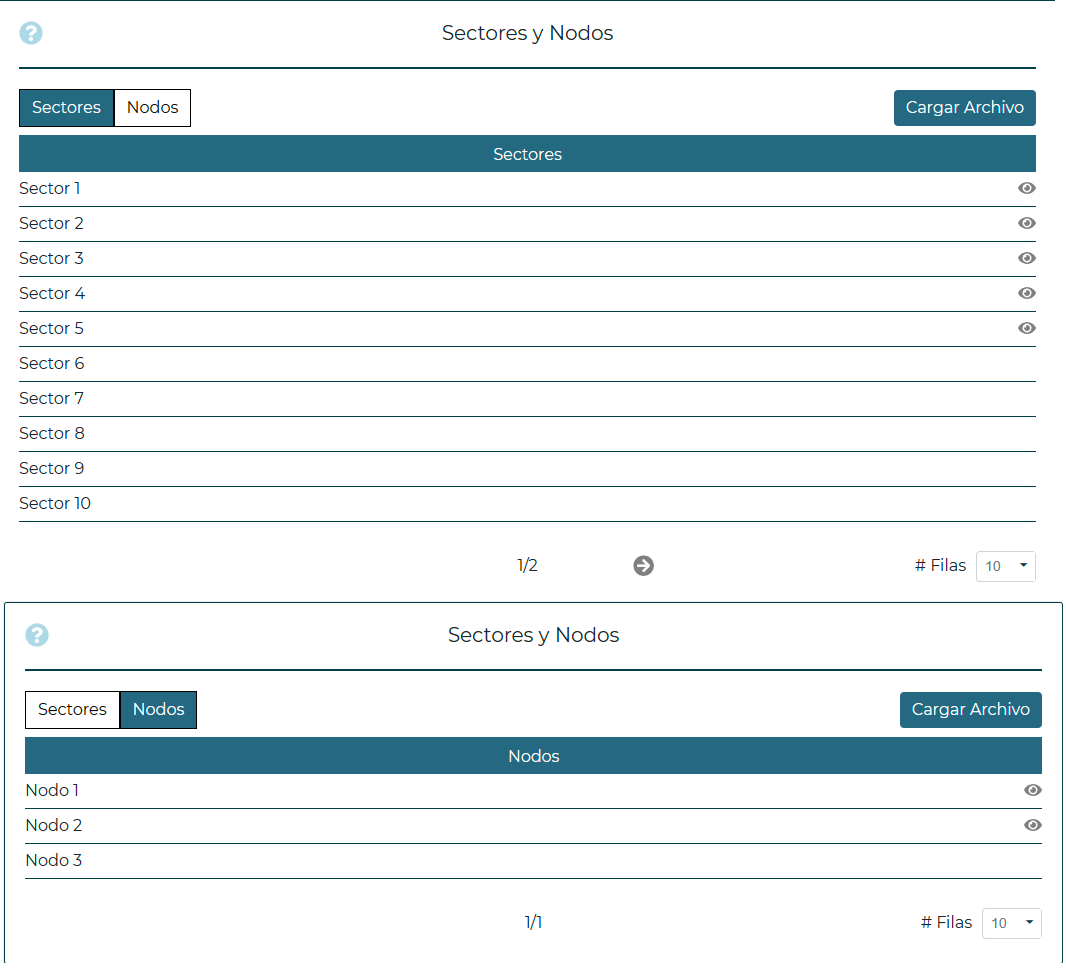
\includegraphics[width=0.8\textwidth]{mapcfg-tables}
	\caption{\label{fig:mapcfg-tables-exameple} Ejemplo tabla de sectores y nodos. Fuente: Elaboración propia.}
\end{figure}


Respecto al mapa, este muestra los sectores y/o nodos que estaban previamente asignados, los sectores los muestra con un color verde (Figura \ref{fig:mapcfg-zone-pre}), mientras que los nodos los muestra con su ícono respectivo (fig). Si esta seleccionada la tabla de sectores en el mapa se muestran solo los polígonos, mismo caso con la tabla de nodos.
\begin{figure}[H]
	\centering
	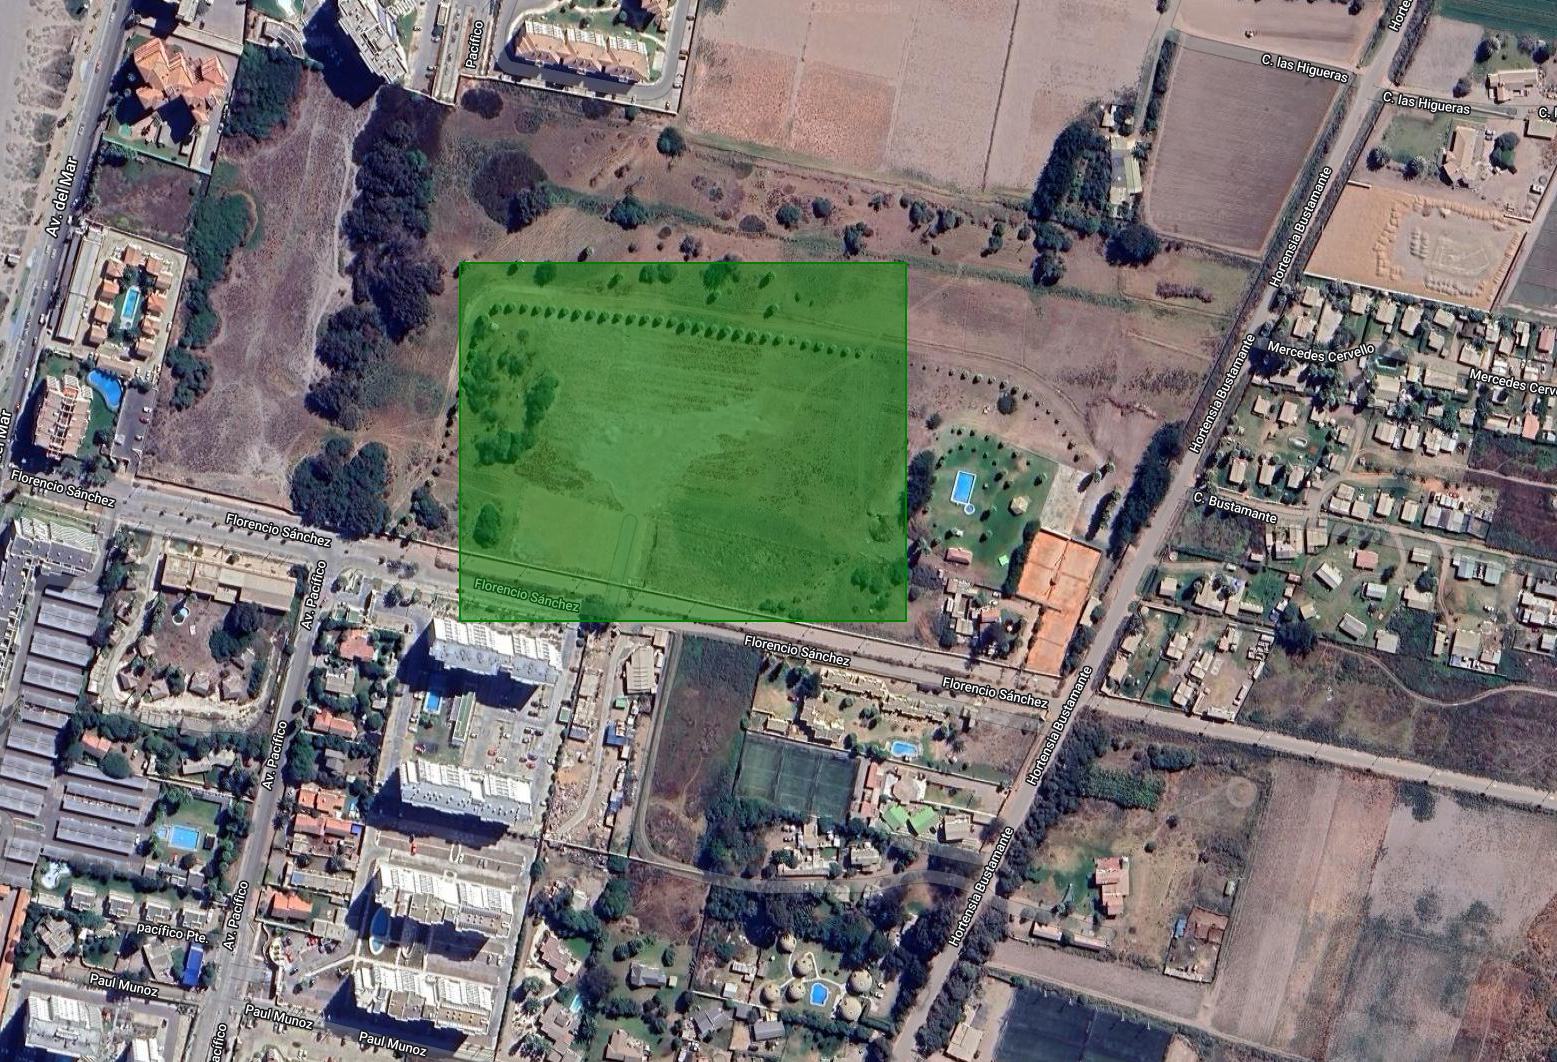
\includegraphics[width=0.8\textwidth]{mapcfg-zone-pre}
	\caption{\label{fig:mapcfg-zone-pre} Sector previamente asignado en el mapa}
\end{figure}

Al cargar un archivo, las secciones cambian. En la tabla de sectores/nodos ocurre lo siguiente (Figura \ref{fig:mapcfg-tables-edit-exameple}):

\begin{itemize}
    \item El botón de "Cargar Archivo" desaparece y se reemplaza por el nombre del archivo cargado junto a un ícono de basura que al hacerle click, elimina el archivo y vuelve al estado anterior.
    \item En la tabla ocurre lo siguiente:
    \begin{itemize}
        \item Se agrega una columna nueva al medio, que contiene un dropdown con los polígonos o nodos (según la tabla seleccionada) del archivo que se cargó recientemente.
        \item En la columna de acciones:
        \begin{itemize}        
            \item Cuando un sector/nodo tiene un polígono/punto previamente asignado, tiene las acciones de centrar en el mapa y descartar polígono/punto.
            \item Al descartar un polígono/punto previamente asignado, el botón de descartar se reemplaza por el botón de volver a polígono/punto original.
            \item Para sectores/nodos que tengan asignados polígonos/puntos, tienen disponible el botón para centrar en el mapa.
        \end{itemize}
    \end{itemize}
    \item En el mapa se agregan los polígonos/puntos del archivo cargado previamente. Para los polígonos se muestran como en la figura \ref{fig:mapcfg-zone-loaded}, mientras que los nodos como en la figura \ref{fig:mapcfg-node-loaded}.
    \item Por último, debajo de la tabla se muestra el botón para guardar los cambios hechos en el mapa, al hacer click sobre este se abrirá un diálogo de confirmación que al ser aceptado se guardarán los cambios y la herramienta volverá al estado en que no había un archivo cargado.
\end{itemize}

\begin{figure}[H]
	\centering
	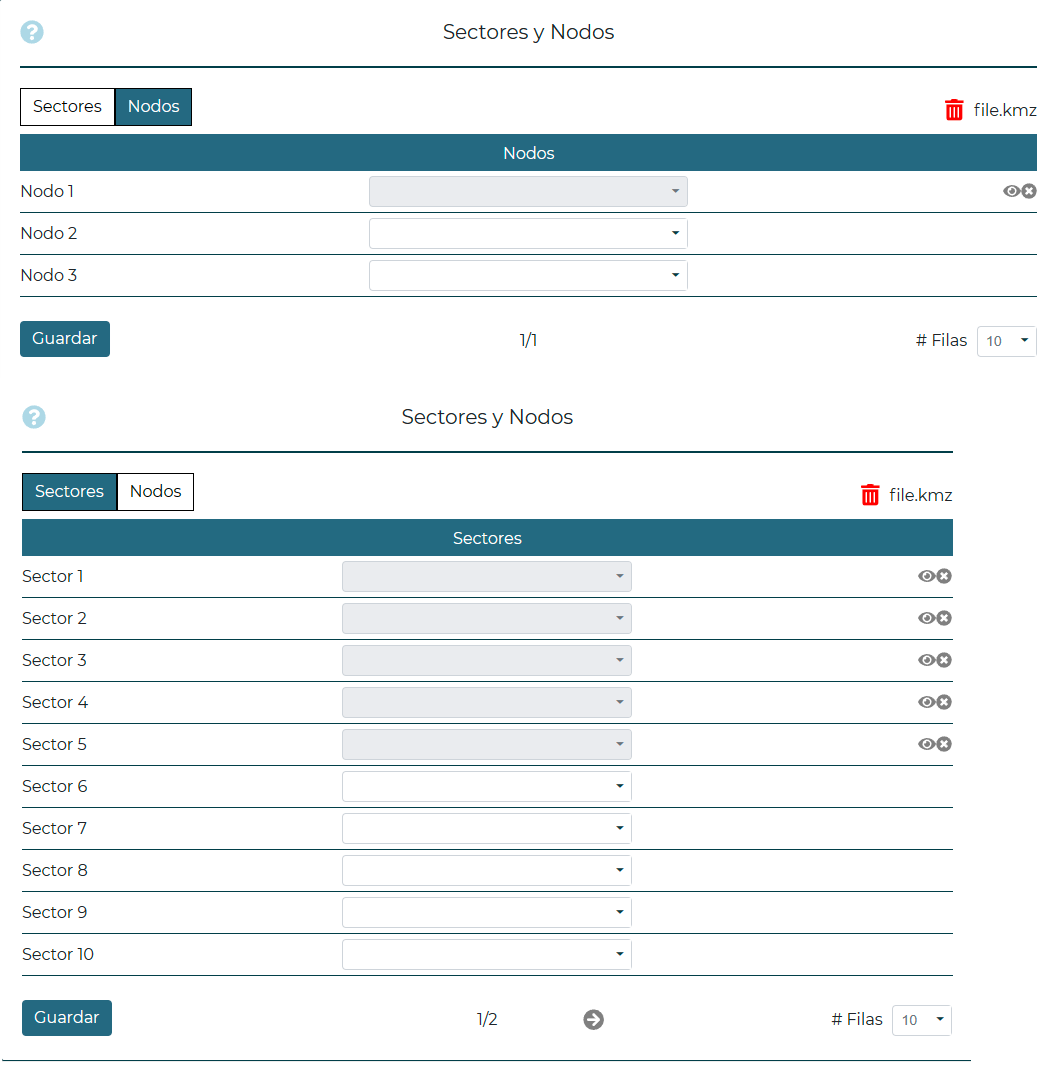
\includegraphics[width=0.8\textwidth]{mapcfg-tables-edit}
	\caption{\label{fig:mapcfg-tables-edit-exameple} Ejemplo tabla de sectores y nodos al cargar un archivo. Fuente: Elaboración propia.}
\end{figure}

\begin{figure}[H]
	\centering
	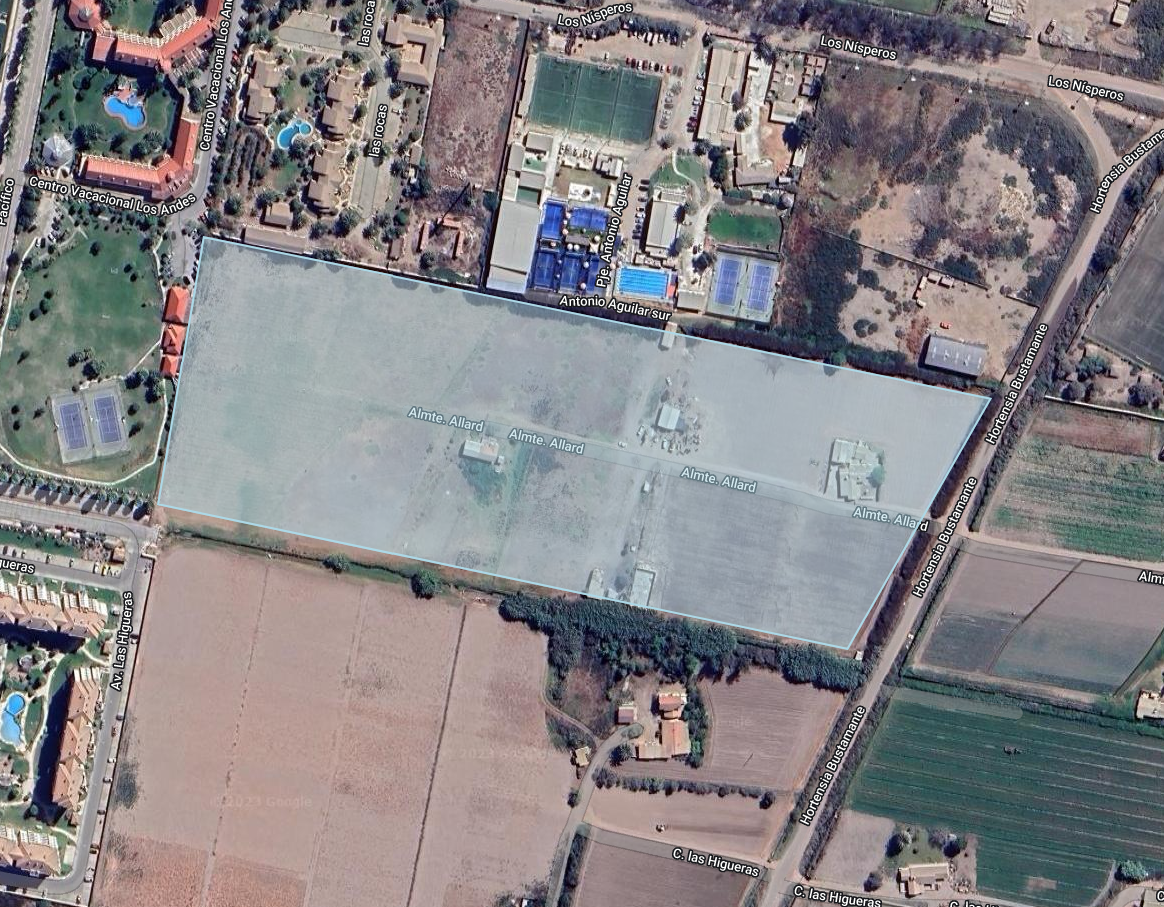
\includegraphics[width=0.8\textwidth]{mapcfg-zone-loaded}
	\caption{\label{fig:mapcfg-zone-loaded} Polígono cargado en el mapa}
\end{figure}

\begin{figure}[H]
	\centering
	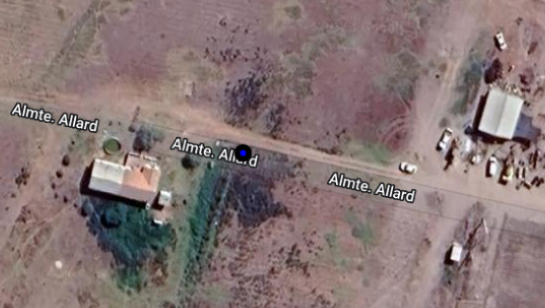
\includegraphics[width=0.8\textwidth]{mapcfg-node-loaded}
	\caption{\label{fig:mapcfg-node-loaded} Punto cargado en el mapa}
\end{figure}

Para la acción de centrar un sector/nodo en el mapa, los polígonos/puntos se verán de la siguiente forma:
\begin{itemize}
    \item Sector previamente asignado (Figura \ref{fig:mapcfg-zone-pre-center}).
    \item Nodo previamente asignado (Figura \ref{fig:mapcfg-node-pre-center}).
    \item Polígono cargado (Figura \ref{fig:mapcfg-zone-loaded-center}).
    \item Punto cargado (Figura \ref{fig:mapcfg-node-loaded-center}).
\end{itemize}

\begin{figure}[H]
	\centering
	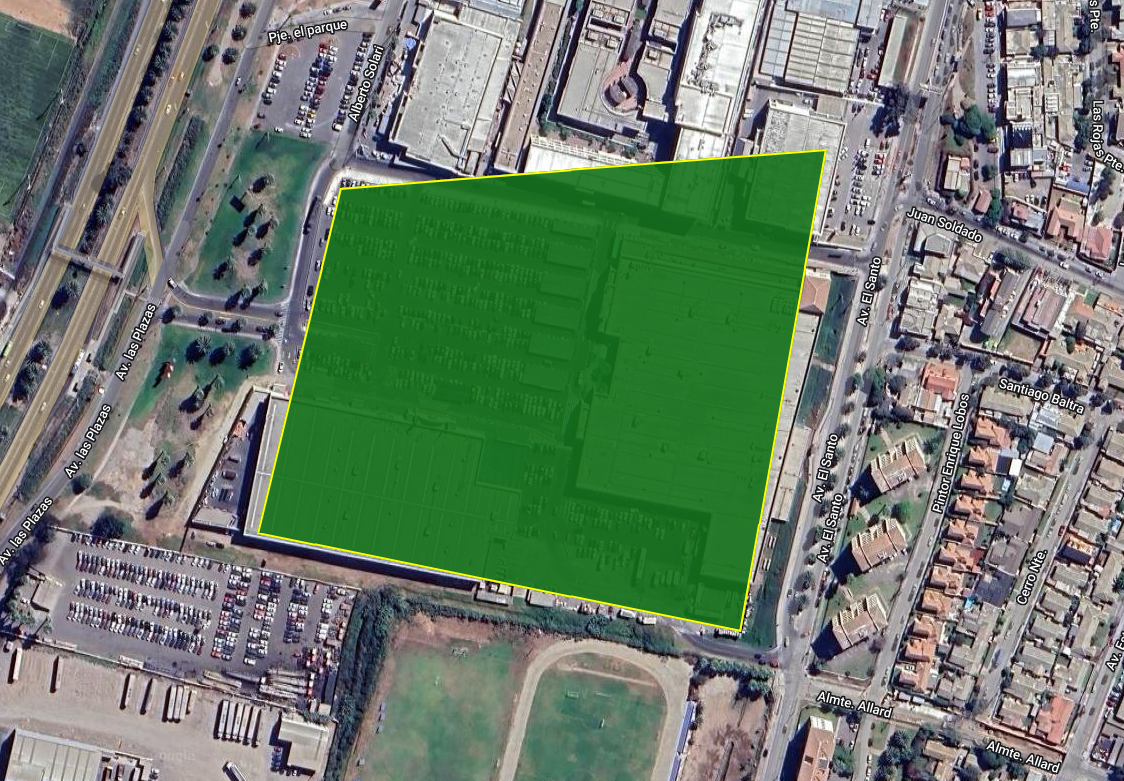
\includegraphics[width=0.8\textwidth]{mapcfg-zone-pre-center}
	\caption{\label{fig:mapcfg-zone-pre-center} Sector previamente asignado centrado en el mapa}
\end{figure}

\begin{figure}[H]
	\centering
	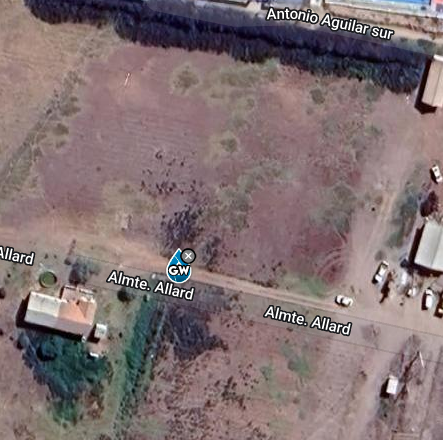
\includegraphics[width=0.8\textwidth]{mapcfg-node-pre-center}
	\caption{\label{fig:mapcfg-node-pre-center} Nodo previamente asignado centrado en el mapa}
\end{figure}

\begin{figure}[H]
	\centering
	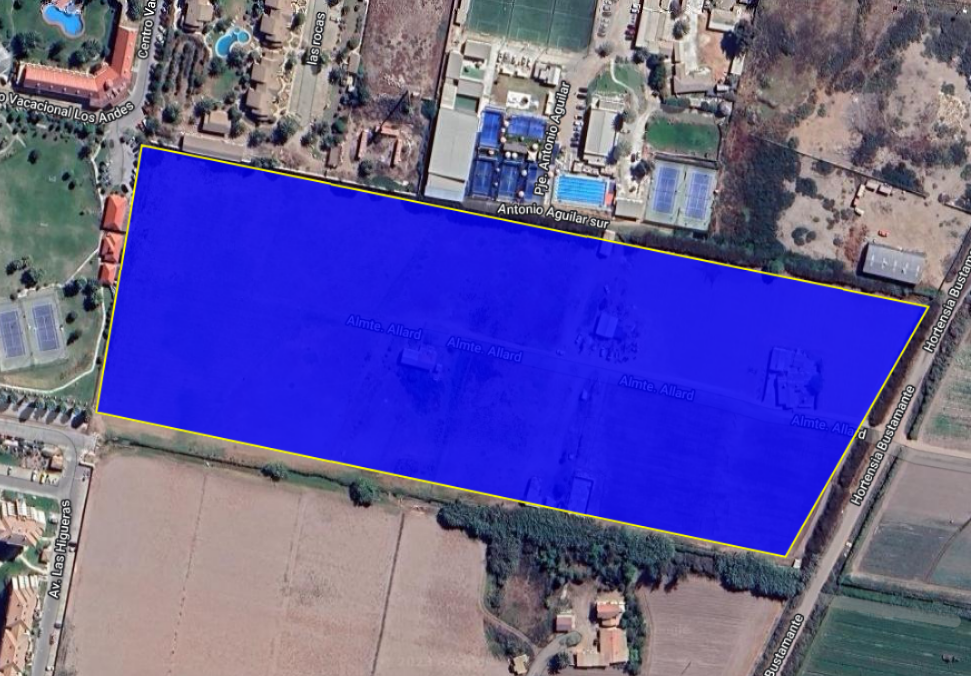
\includegraphics[width=0.8\textwidth]{mapcfg-zone-loaded-center}
	\caption{\label{fig:mapcfg-zone-loaded-center} Polígono cargado centrado en el mapa}
\end{figure}

\begin{figure}[H]
	\centering
	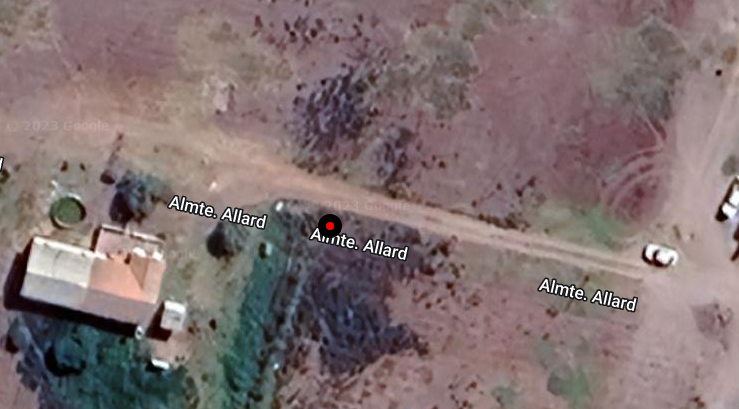
\includegraphics[width=0.8\textwidth]{mapcfg-node-loaded-center}
	\caption{\label{fig:mapcfg-node-loaded-center} Punto cargado centrado en el mapa}
\end{figure}

Para finalizar, al hacer click en el botón 'Guardar', se abrirá un diálogo de confirmación para confirmar, valga la redundancia, los cambios hechos y guardarlos.

\iffalse
\subsubsection{ALINEADOR DE IMÁGENES}

Una de las herramientas que ofrece \textit{DropControl} es el análisis de imágenes utilizando
el índice de vegetación de diferencia normalizada o NDVI\footnote{\href{https://eos.com/es/make-an-analysis/ndvi/}{NDVI: Índice De Vegetación De Diferencia Normalizada}} por sus siglas en inglés. Para obtener estas imágenes satelitales
se utilizan otros proveedores y se muestran en \textit{DropControl} con \textit{Google Maps}, pero no todas las imágenes tienen
las mismas coordenadas en \textit{Google Maps} por lo que se verán desalineadas. Esto se hace mandando un ticket al área de soporte
y son ellos lo que se encargan de alinear la imagen.

La solución para este problema se plantea una nueva herramienta para la aplicación de \textit{Admin de DropControl} en la que
se puedan alinear las imágenes satelitales a \textit{Google Maps}.

Esta nueva herramienta se encontrará en la sección de 'Proveedores Externos'. (Explicar un poco como funciona esta herramienta.). Al hacer click sobre un proveedor externo se abre un diálogo con información de este, si tiene fecha de 'Último vuelo', tendrá disponible el botón de 'Alinear imágen' el cual redireccionará a la herramienta en cuestión.

En esta herramienta contiene un mapa del campo, en Google Maps, con polígonos determinando los sectores de este. Sobre el mapa estará la imagen satelital del proveedor externo, el cual se podrá mover para que el usuario pueda alinearlo con el mapa de Google Maps.
En el mapa se pueden hacer las siguientes acciones:
\begin{itemize}
    \item Haciendo CTRL + click sobre la imágen satelital del proveedor externo, se puede mover la imagen.
    \item En la esquina superior derecha del mapa se encuentra un \textit{slider} de opacidad de la imagen, para poder contrastar mejor la imagen satelital con el mapa.
\end{itemize}

Cuando el usuario logre alinear la imágen como el desee, debe hacer click en el botón 'Guardar' el cual abrirá un diálogo de confirmación para confirmar los cambios.

Los cambios se verán reflejados en la herramienta de análisis de imágenes en DropControl.
\fi
\subsubsubsection{GRAFICADOR LIBRE}

Como se explicó anteriormente, el plan gratuito que ofrece \textit{Wiseconn} sirve como punto de entrada a las herramientas
de pago de \textit{DropControl}. Sin embargo, el plan gratuito ofrece muy pocas funcionalidades y/o herramientas
implicando poca retención de los usuarios y no se cumplen con las especificaciones comerciales.

Los usuarios clientes de plan de pago tienen a su disposición un graficador en la aplicación de \textit{DropControl} (Figura \ref{fig:graf-drop-classic}), en el cual
se pueden graficar los datos enviados por los nodos en los campos dentro de un rango de tiempo.
Caso contrario ocurre para los usuarios clientes de plan gratuito, los cuales no poseen esta herramienta y
no pueden visualizar los datos de sus nodos.

\begin{figure}[H]
	\centering
	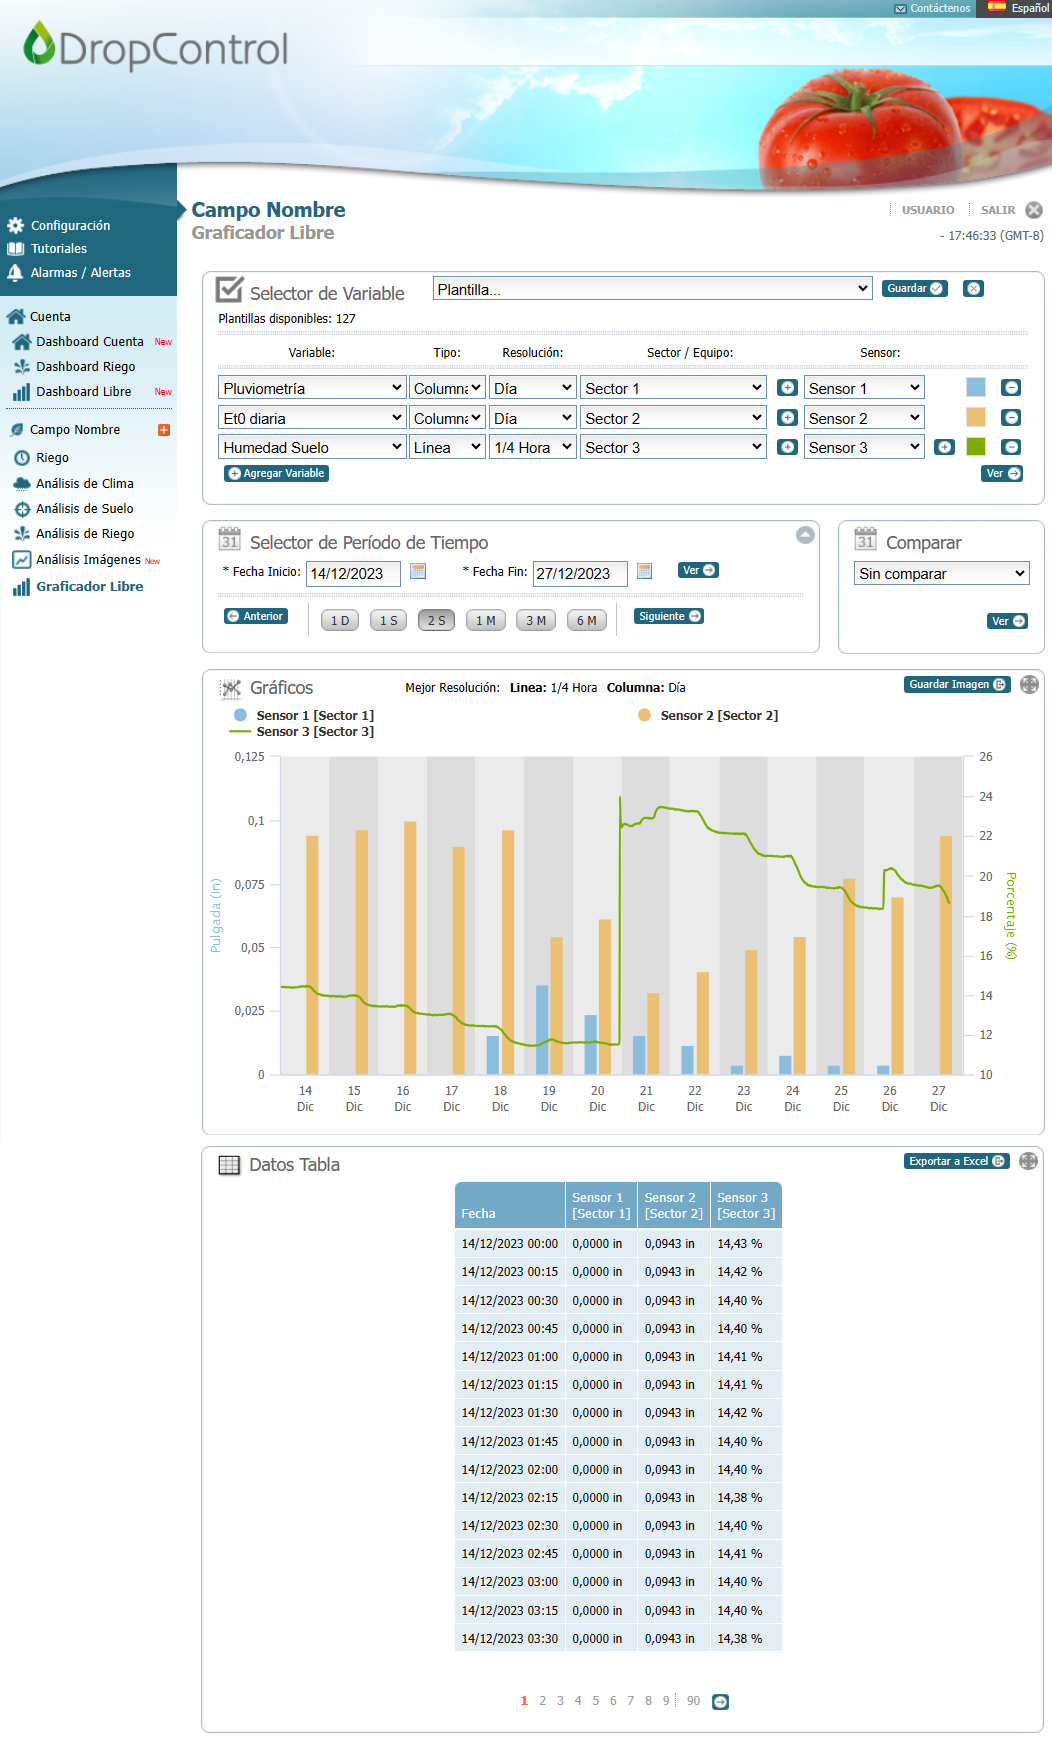
\includegraphics[width=0.5\textwidth]{graf-drop-classic}
	\caption{\label{fig:graf-drop-classic} Graficador Libre en \textit{DropControl}}
\end{figure}

Por esto se desarrolla la herramienta de 'Graficado Libre' en la aplicación de \textit{Admin de DropControl},
donde el usuario podrá escoger hasta 6 sensores para graficar en un rango de tiempo máximo de los últimos 3 meses (90 días).

Esta nueva herramienta se podrá acceder en el menú de \textit{Admin de DropControl} como muestra en la figura \ref{fig:menu-admin-graf1} bajo el nombre de `Graficador Libre`. 

\begin{figure}[H]
	\centering
	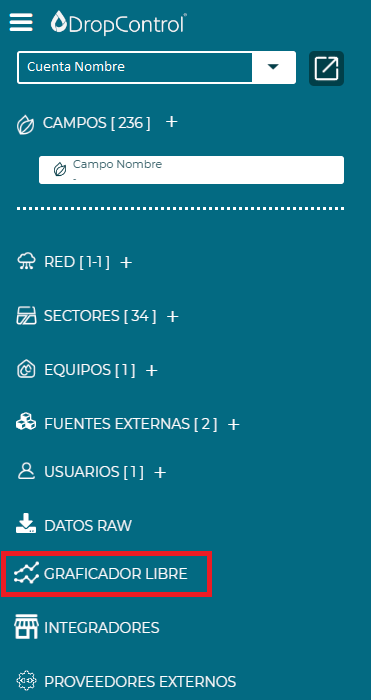
\includegraphics[width=0.5\textwidth]{menu-admin-graficador}
	\caption{\label{fig:menu-admin-graf1} Graficador Libre en el menú de \textit{Admin}}
\end{figure}

El graficador libre tendrá el siguiente esquema mostrado en la figura \ref*{fig:graf-esquema}

\begin{figure}[H]
	\centering
	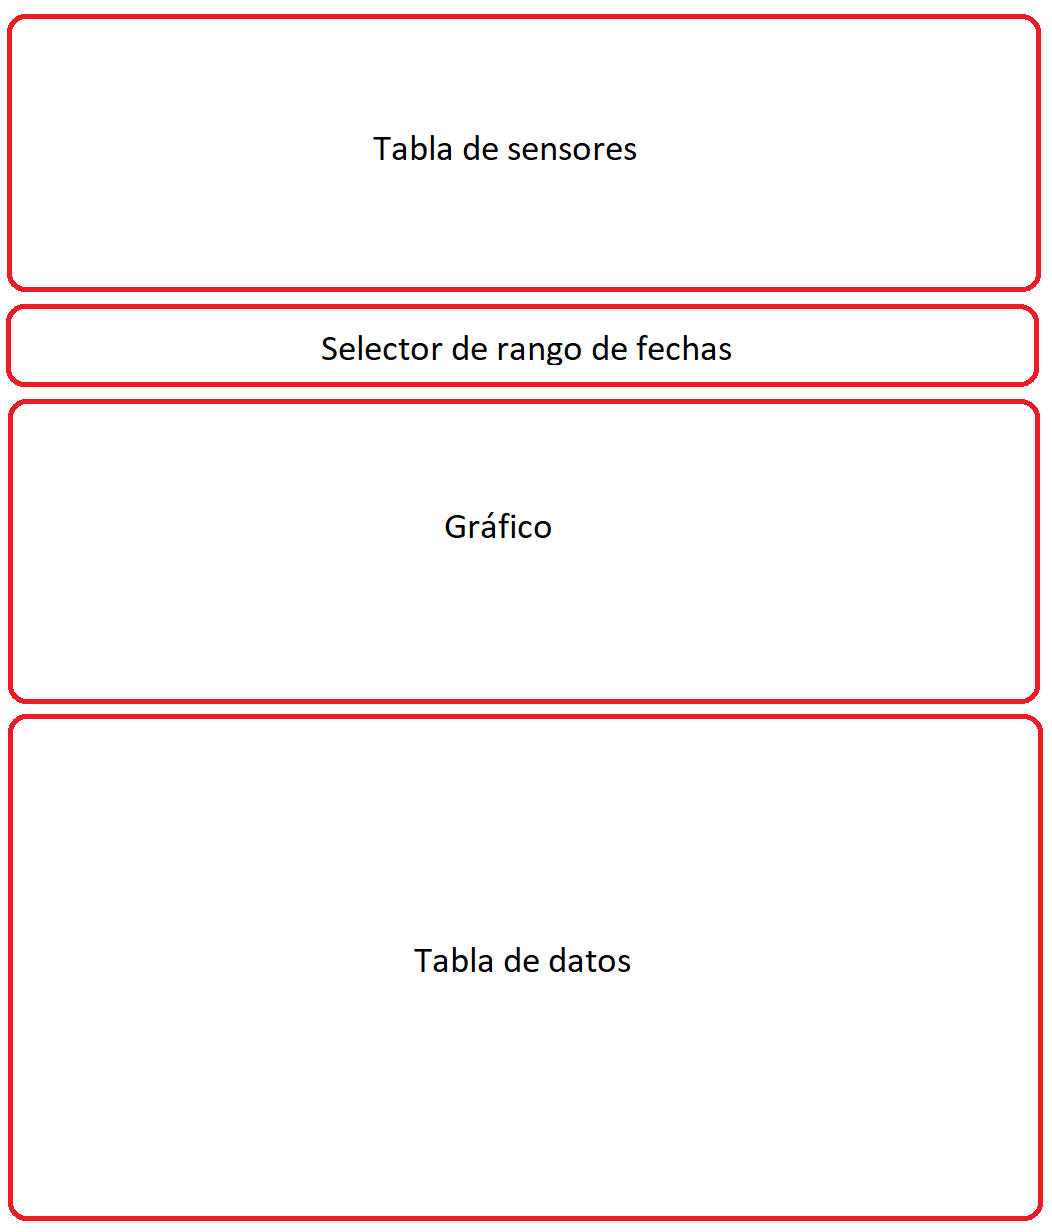
\includegraphics[width=0.5\textwidth]{graf-esquema}
	\caption{\label{fig:graf-esquema} Esquema graficador libre. Fuente: Elaboración propia.}
\end{figure}

En la tabla de sensores es donde se seleccionan los sensores que se quieren desplegar en el gráfico. Esta tabla tiene las siguientes propiedades y componentes (Figura \ref{fig:graf-table}):
\begin{itemize}
    \item En primera instancia, la tabla empieza con una fila (Figura \ref{fig:graf-table-empty}).
    \item Se podrá escoger hasta 6 sensores.
    \item Las columnas de la tabla son las siguientes:
          \begin{enumerate}
              \item Selector de nodos.
              \item Selector de sensores.
              \item Selector de color.
              \item Botón para eliminar fila (Aparece cuando se tiene más de una fila).
          \end{enumerate}
    \item Botón para agregar una fila vacía.
\end{itemize}

\begin{figure}[H]
	\centering
	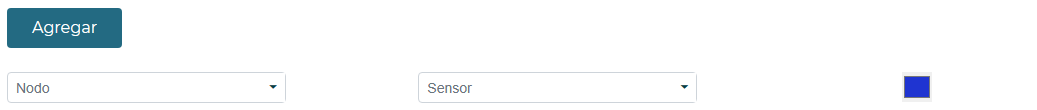
\includegraphics[width=0.5\textwidth]{graf-table-empty}
	\caption{\label{fig:graf-table-empty} Tabla de sensores vacía. Fuente: Elaboración propia.}
\end{figure}

\begin{figure}[H]
	\centering
	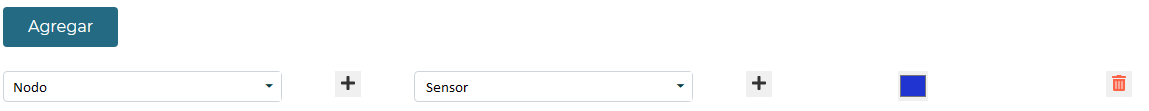
\includegraphics[width=0.5\textwidth]{graf-table}
	\caption{\label{fig:graf-table} Componentes de la tabla de sensores. Fuente: Elaboración propia.}
\end{figure}

Los sensores pertenecen a un nodo, es por esto que primero se debe seleccionar el nodo en el primer selector, para luego seleccionar el sensor perteneciente a ese nodo.
Para agregar nuevas filas a la tabla de sensores existen 3 formas.
\begin{enumerate}
    \item Haciendo click en el botón de `Agregar fila` que está en la esquina superior derecha de la tabla.
    \item Al escoger un nodo, al lado del selector aparecerá un botón con el signo `+` (Figura \ref{fig:graf-table}). Al hacer click en ese botón agregará una nueva fila con el nodo siguiente en la lista seleccionado.
    \item Al escoger un sensor, al lado del selector aparecerá un botón con el signo `+` (Figura \ref{fig:graf-table}). Al hacer click en ese botón agregará una nueva fila con el nodo seleccionado en la fila anterior junto al sensor siguiente en la lista.
\end{enumerate}

En cuanto al selector de rango de fecha (Figura \ref{fig:graf-chart-daterange-example}), se podrá escoger un máximo de los últimos 90 días. Además, existirán rangos predeterminados para que el usuario pueda escoger:
\begin{itemize}
    \item Últimos 7 días.
    \item Este mes.
    \item Últimos 30 días.
    \item Últimos 60 días.
    \item Últimos 90 días.
\end{itemize}
Para esto se utilizará el componente \textit{DateRangePicker} de \textit{Syncfusion}\footnote{\href{https://ej2.syncfusion.com/react/documentation/daterangepicker/getting-started}{Syncfusion: DateRangePicker}}.
\begin{figure}[H]
	\centering
	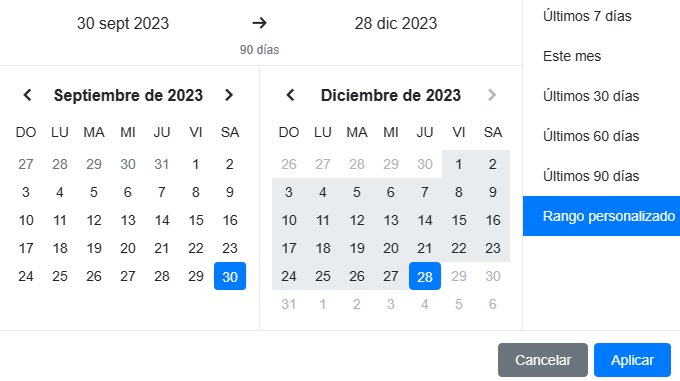
\includegraphics[width=0.5\textwidth]{graf-chart-daterange-example}
	\caption{\label{fig:graf-chart-daterange-example} Ejemplo de componente \textit{DateRangePicker}. Fuente: Elaboración propia.}
\end{figure}
Respecto al gráfico, se utilizará \textit{Highcharts Stock}\footnote{\href{https://www.highcharts.com/docs/stock/understanding-highcharts-stock}{Understanding Highcharts Stock}} para poder desplegar los datos. Cada serie del gráfico representa un sensor que se escogió en la tabla de sensores. La serie tendra un formato de nombre [Nodo]-[Sensor].
\begin{figure}[H]
	\centering
	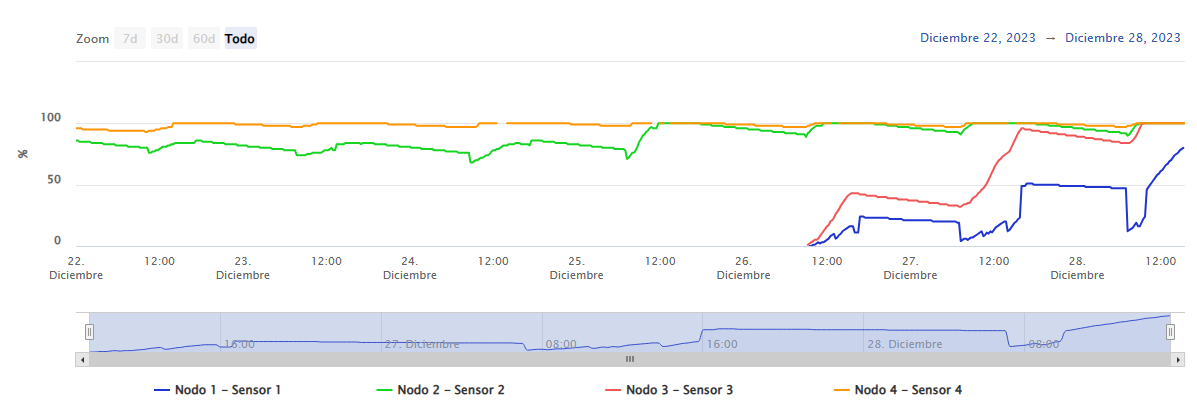
\includegraphics[width=0.5\textwidth]{graf-chart-example}
	\caption{\label{fig:graf-chart-example} Ejemplo de gráfico. Fuente: Elaboración propia.}
\end{figure}

Pasar el puntero por encima de las series, mostrará un \textit{tooltip} con el dato de las series (Figura \ref{fig:graf-chart-tooltip}).
\begin{figure}[H]
	\centering
	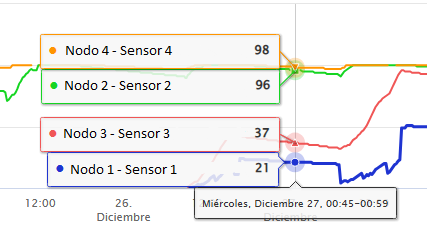
\includegraphics[width=0.5\textwidth]{graf-chart-tooltip}
	\caption{\label{fig:graf-chart-tooltip} \textit{Tooltip}. Fuente: Elaboración propia.}
\end{figure}
Al estar usando \textit{Highcharts Stock}, nos permite realizar las siguientes acciones:
\begin{itemize}
    \item Se podrá hacer zoom, ya sea, de forma manual seleccionado el rango en el gráfico o haciendo click en las opciones para ver rangos de 7, 30, 60 días en la esquina superior izquierda (dependiendo del rango de fechas seleccionado). También se podrá usar el \textit{navigator}\footnote{\href{https://www.highcharts.com/docs/stock/navigator}{Highcharts Stock Navigator}} que proporciona la librería
    \item Esconder/mostrar series del gráfico haciendo click en la leyenda de la serie.
\end{itemize}

Por último tenemos la tabla de datos del gráfico (Figura \ref{fig:graf-chart-table-example}), para esto se utilizará el componente \textit{Grid}\textit{Syncfusion}\footnote{\href{https://ej2.syncfusion.com/react/documentation/grid/getting-started}{Syncfusion: Grid}} de \textit{Syncfusion}, que nos permite agregar la acción de \textit{Sorting} por columna y exportar la tabla en formato .xls.
La tabla tiene las siguientes propiedades:
\begin{itemize}
    \item La primera columna corresponde a la fecha y las columnas siguientes corresponden a las combinaciones de nodos/sensores seleccionados.
    \item La tabla es paginada y se puede cambiar el número de filas que se pueden mostrar por cada página.
    \item La tabla se ordena por fecha del dato, el cual se puede cambiar el orden haciendo click en el header de la columna.
    \item En la esquina superior derecha habrá un botón con el cual se podrá descargar la tabla en formato .xls.
\end{itemize}

\begin{figure}[H]
	\centering
	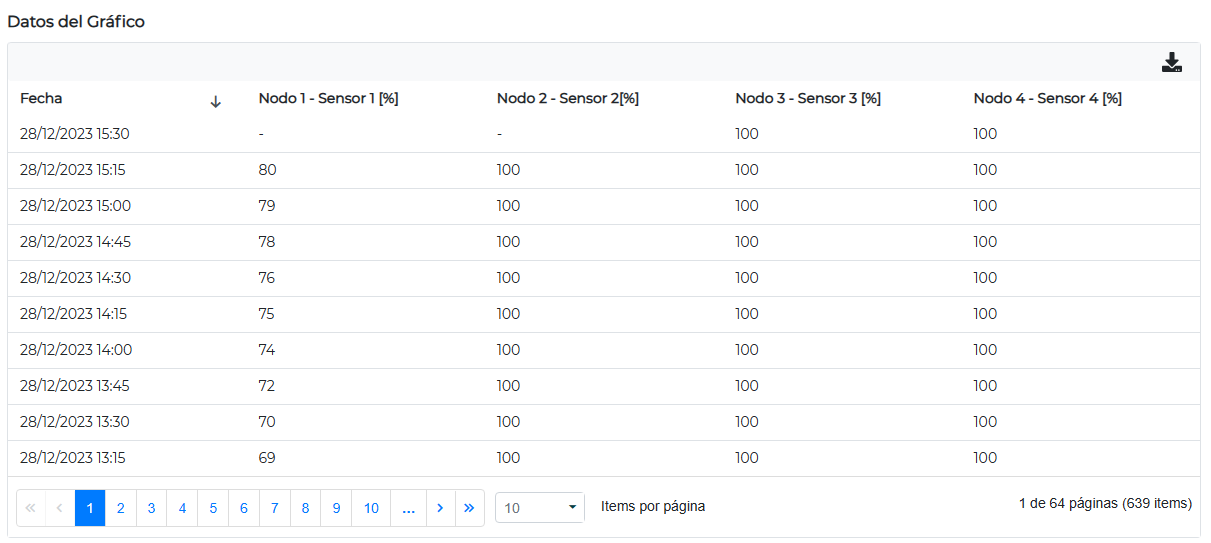
\includegraphics[width=0.5\textwidth]{graf-chart-table-example}
	\caption{\label{fig:graf-chart-table-example} Ejemplo de tabla de datos. Fuente: Elaboración propia.}
\end{figure}

\subsubsection{OPERATIONS}

El área de producción se encarga del ensamblado y testeo del hardware de WiseConn junto con el su inventario y despachos de estos. Para llevar registro de todo esto se utiliza la aplicación de \textit{Operations}

En \textit{Operations} se puede hacer:

\begin{itemize}
    \item Configurar los tipos de productos.
    \item Administrar lotes de productos.
    \item Administrar despachos de productos.
    \item Llevar el inventario de los productos y los estados de estos, gracias a que cada producto tiene asociado un historial.
\end{itemize}

\subsubsubsection{DESPACHOS MÚLTIPLES}

En \textit{Operations}, como se mencionó anteriormente, se administran los despachos de los distintos productos de hardware que ofrece \textit{WiseConn}.
La sección de despachos (Figura \ref{fig:dm-mantenedor-indv}) se compone de una tabla que contiene los despachos, valga la redundancia, creados. La tabla contiene botónes de acciones de crear, editar, eliminar y exportar a CSV en el \textit{header} y \textit{footer} de este, además, en la parte izquierda del \textit{header} existe un filtro de rango de fecha. 
Para las acciones de ver, eliminar y cerrar es necesario primero seleccionar una fila de la tabla para que se habilite el botón.
De igual manera, existen filtros por columnas como se ve en la figura \ref{fig:dm-mantenedor-indv-filters}.

\begin{figure}[H]
	\centering
	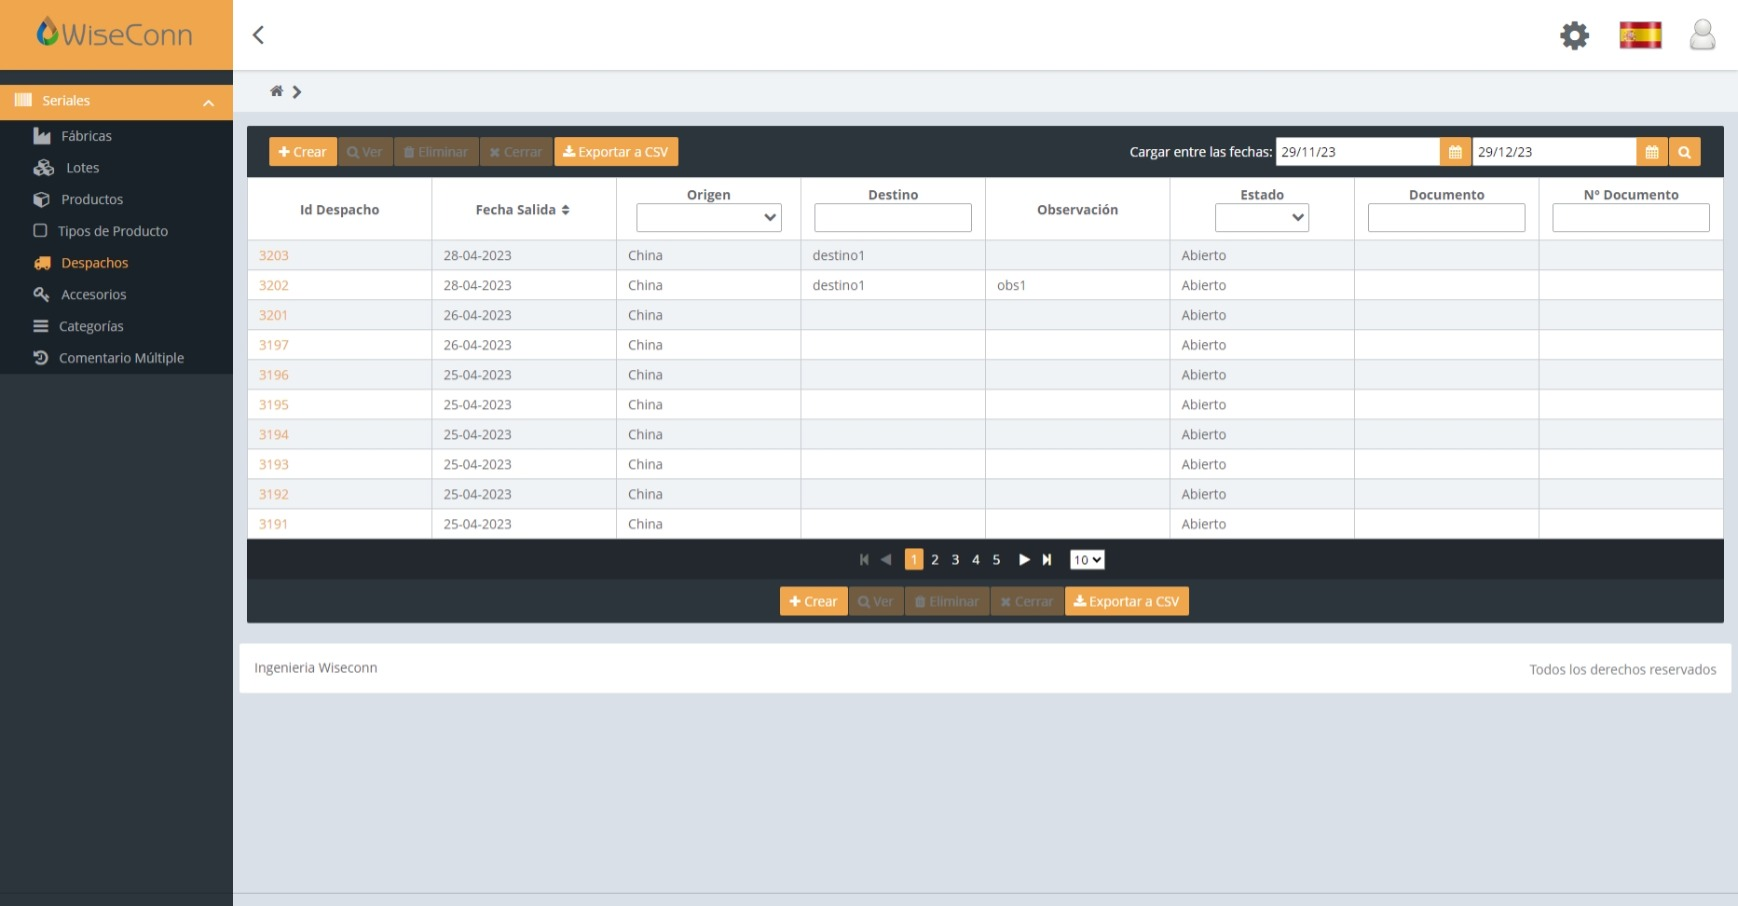
\includegraphics[width=0.5\textwidth]{dm-mantenedor-indv}
	\caption{\label{fig:dm-mantenedor-indv} Sección de despachos. Fuente: Elaboración propia.}
\end{figure}

\begin{figure}[H]
	\centering
	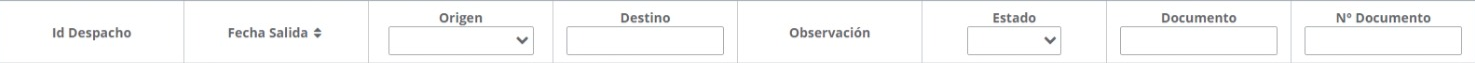
\includegraphics[width=0.5\textwidth]{dm-mantenedor-indv-filters}
	\caption{\label{fig:dm-mantenedor-indv-filters} Filtros por columna. Fuente: Elaboración propia.}
\end{figure}

Al hacer click en el botón crear se abre un siguiente formulario (Figura \ref{fig:dm-create-indv-form}) para ingresar las propiedades:
\begin{itemize}
    \item Fecha de salida
    \item Fecha de activación
    \item Destino
    \item País destino
    \item Observación
    \item Documento
    \item Número de documento
    \item Despacho interno \textit{flag}    
\end{itemize}

\begin{figure}[H]
	\centering
	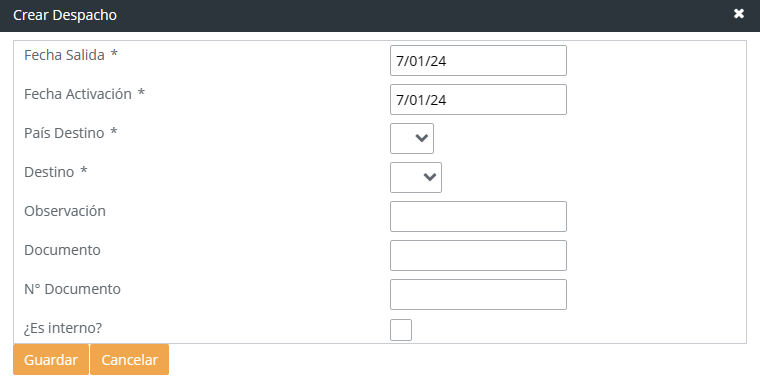
\includegraphics[width=0.5\textwidth]{dm-create-indv-form}
	\caption{\label{fig:dm-create-indv-form} Filtros por columna. Fuente: Elaboración propia.}
\end{figure}

Para poder entrar a un despacho se debe hacer click en la fila de la tabla y hacer click en el botón ver, al igual que haciendo click en la Id del despacho.
La vista del despacho se muestra en la figura \ref{fig:dm-vista-indv}.

\begin{figure}[H]
	\centering
	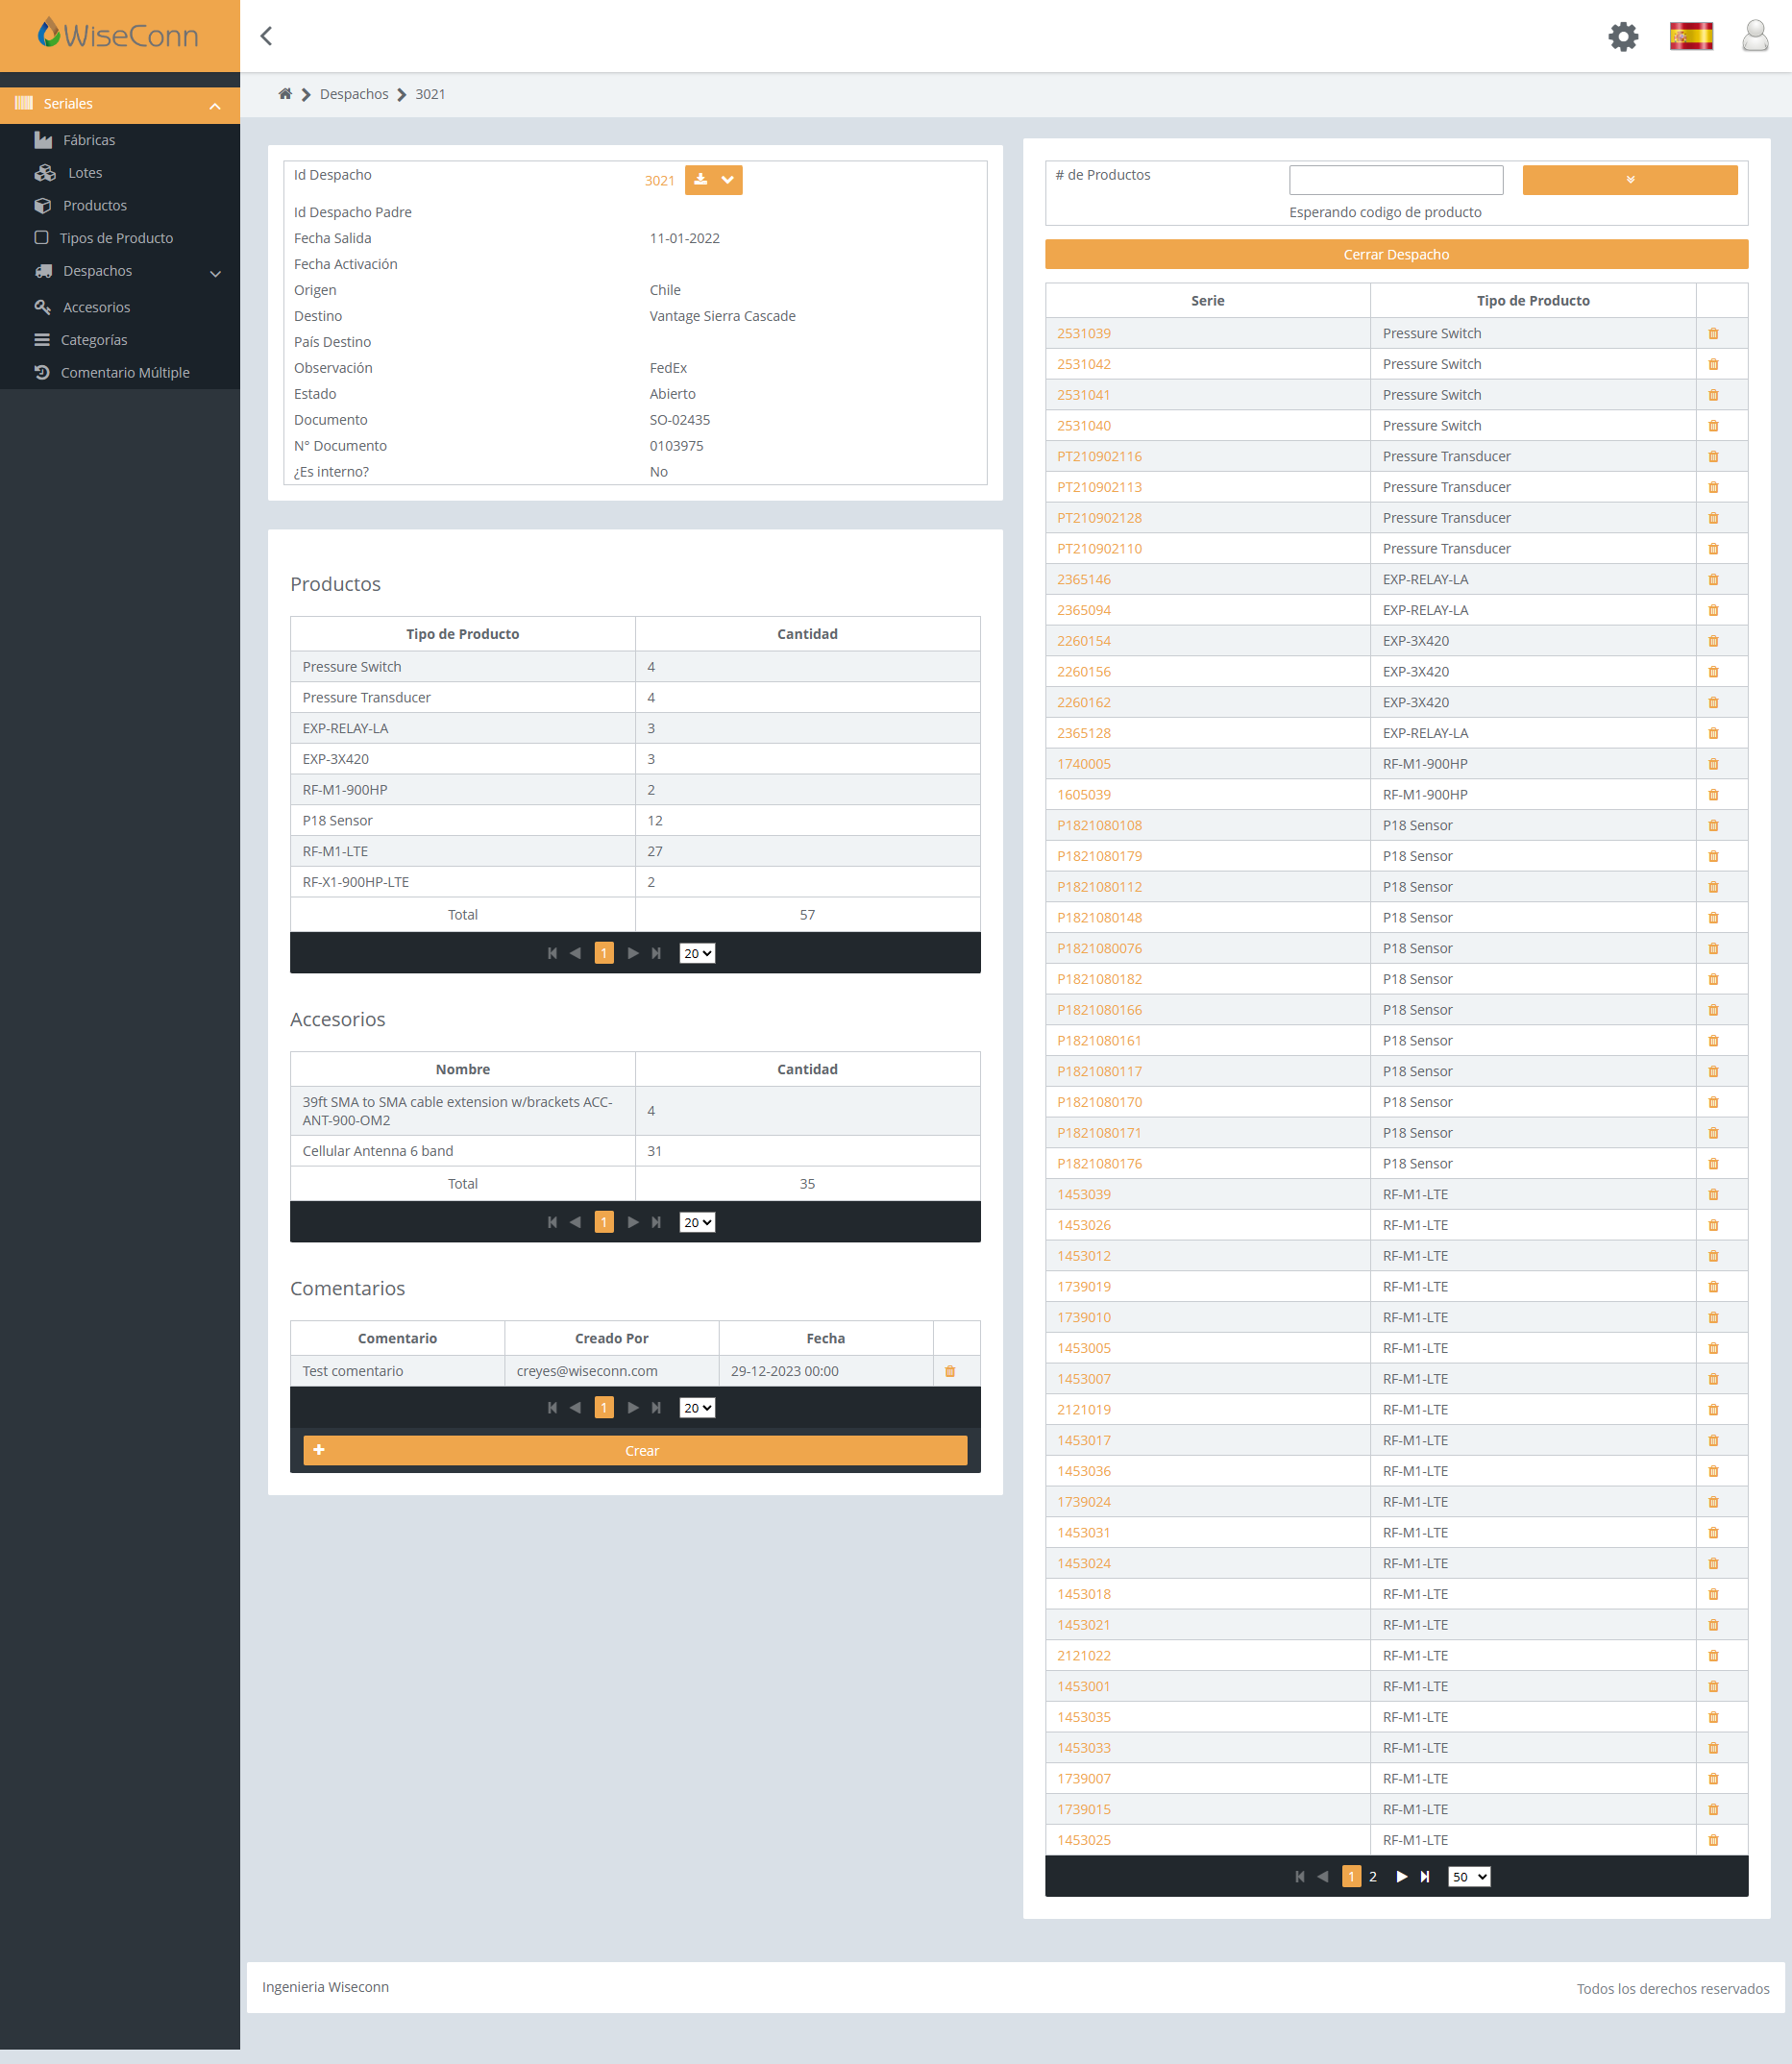
\includegraphics[width=0.5\textwidth]{dm-vista-indv}
	\caption{\label{fig:dm-vista-indv} Vista de despacho. Fuente: Elaboración propia.}
\end{figure}

La vista del despacho contiene las siguientes secciones:
\begin{itemize}
    \item En el lado derecho:
    \begin{itemize}
        \item \textit{Input} para ingresar la serie del producto o código de accesorio.
        \item Tabla de productos. Columnas: Series, tipo de producto, acción de eliminar.
    \end{itemize}
    \item En el lado izquierdo:
    \begin{itemize}
        \item Información del despacho.
        \item Resumen de productos.
        \item Resumen de accesorios.
        \item Tabla de comentarios.
    \end{itemize}
\end{itemize}

En la vista de un despacho se pueden editar las propiedades de este como muestra en la figura \ref{fig:dm-indv-edit}, haciendo click sobre el dato se cambiará a un input correspondiente al tipo de dato (fecha, texto, select, etc.). Agregar productos y accesorios y descargar un reporte.

\begin{figure}[H]
	\centering
	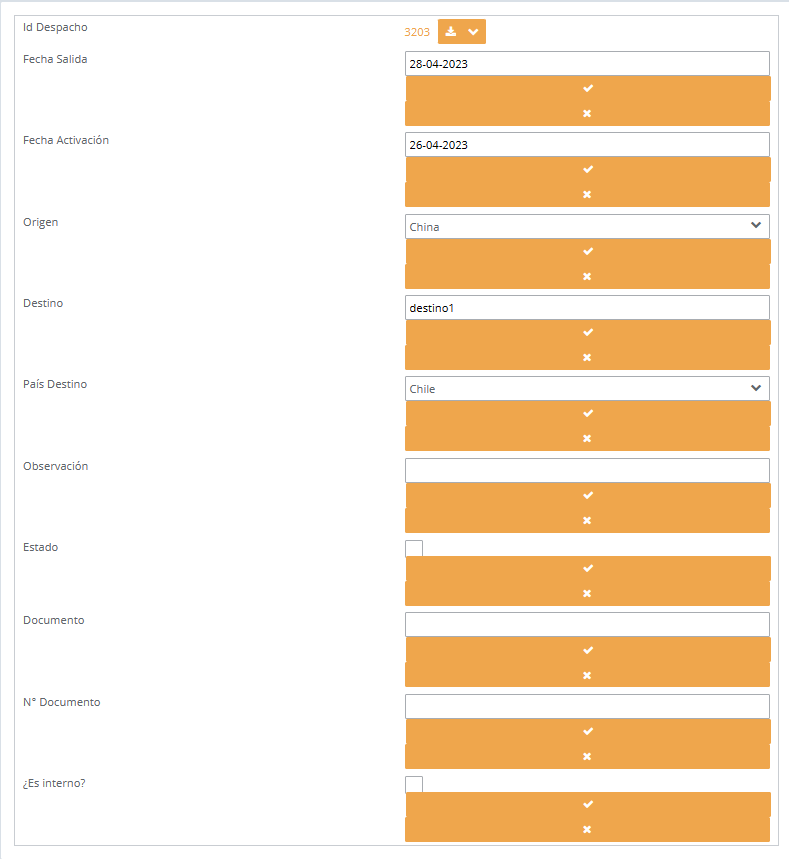
\includegraphics[width=0.5\textwidth]{dm-indv-edit}
	\caption{\label{fig:dm-indv-edit} Edición propiedades despacho. Fuente: Elaboración propia.}
\end{figure}
Existen casos en que no todos los productos deben estar en un mismo despacho y se crean despachos apartes para estos, con el mismo destino y fecha de despacho.
Como en \textit{Operations} el despacho es individual, no existe una forma de agrupar estos despachos que comparten propiedades. Por esto, se plantea crear la funcionalidad de 'Despacho múltiples'. 
Los despachos múltiples tendrán una sección aparte en \textit{Operations}, en el menú lateral los despachos se dividen entre individuales y múltiples.

Al entrar a la sección de despachos múltiples, se muestra la tabla de los despachos múltiples (Figura \ref{fig:dm-mantenedor-mult}) que contiene:
\begin{itemize}
    \item Listado de Despachos Múltiples. Las columnas que se muestran son:
    \begin{itemize}
        \item \textbf{ID de Despacho}
        \item \textbf{Fecha de salida} (Ordenable)
        \item \textbf{Destino} (con filtro de texto)
        \item \textbf{Observación}
        \item \textbf{Estado} (Con filtro seleccionado el estado Abierto/Cerrado/Todos)
    \end{itemize}
    \item Botónes de acción en \textit{header} y \textit{footer} para crear, ver y eliminar despacho.
    \begin{itemize}
        \item \textbf{Crear:} Abre el formulario para crear un despacho múltiple.
        \item \textbf{Ver:} Al seleccionar una fila de la tabla, que corresponde a un despacho, hacer click en esta acción lleva a la vista del despacho múltiple.
        \item \textbf{Eliminar:} Al seleccionar una fila de la tabla, que corresponde a un despacho, hacer click en esta acción elimina el despacho seleccionado (luego de confirmar la acción en un diálogo de confirmación).
    \end{itemize}
    \item Filtro de rango de fechas.
\end{itemize}

\begin{figure}[H]
	\centering
	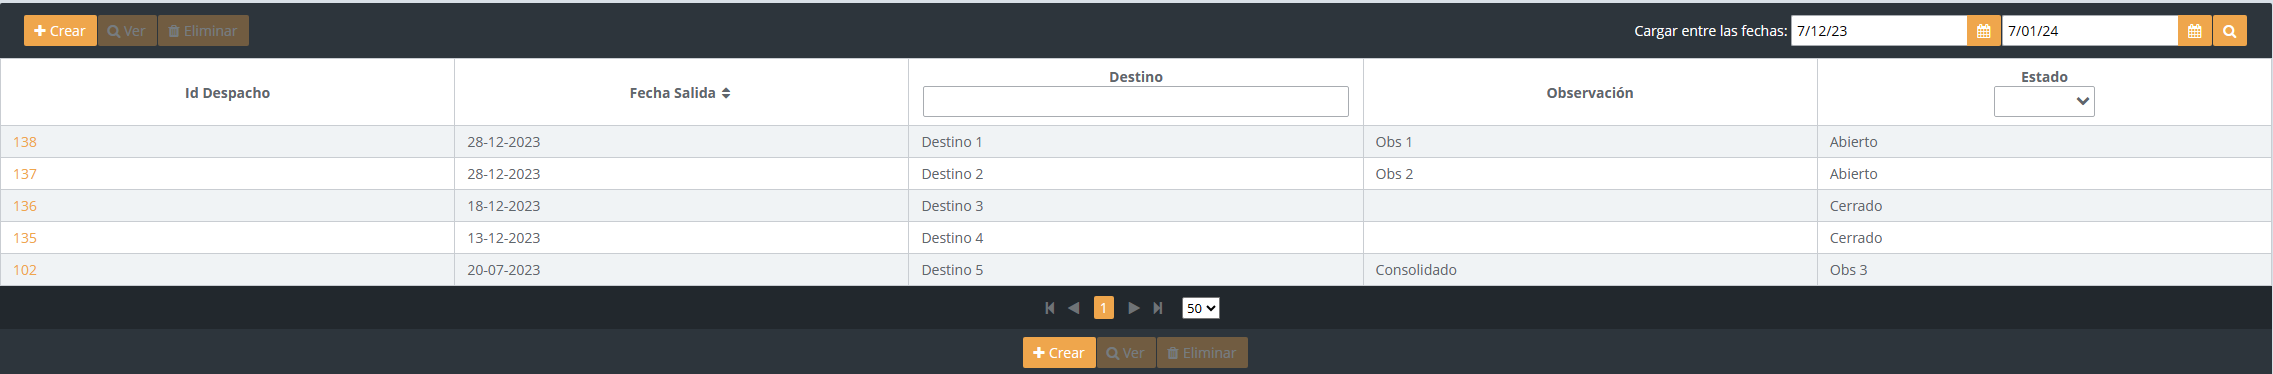
\includegraphics[width=0.5\textwidth]{dm-mantenedor-mult}
	\caption{\label{fig:dm-mantenedor-mult} Sección de despachos múltiples. Fuente: Elaboración propia.}
\end{figure}

En el formulario de creación (Figura \ref{fig:dm-create-multi-form}) se ingresan las siguientes propiedades:
\begin{itemize}
    \item Fecha de salida
    \item Destino
    \item País Destino
    \item Observación (Propia del despacho padre)
    \item Despacho interno \textit{flag}    
    \item Número de despachos.
\end{itemize}

\begin{figure}[H]
	\centering
	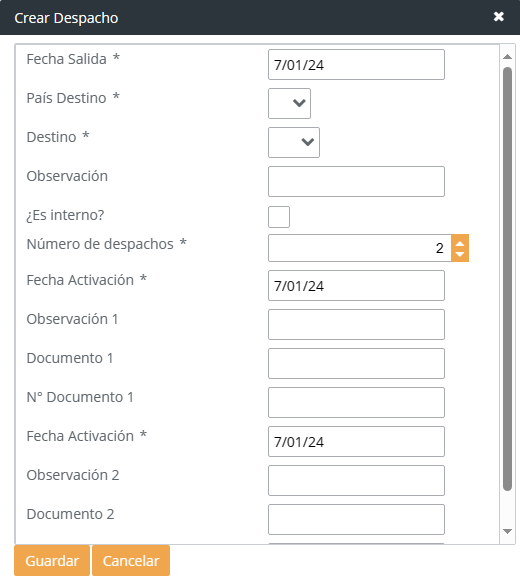
\includegraphics[width=0.5\textwidth]{dm-create-multi-form}
	\caption{\label{fig:dm-create-multi-form} Formulario creación despacho múltiple. Fuente: Elaboración propia.}
\end{figure}

Según el número de despachos hijos ingresado, en el formulario se van agregando campos para cada despacho hijo, diferenciado por un número de creación. Las propiedades individuales de cada despacho hijo son:
\begin{itemize}
    \item Fecha de activación
    \item Observación
    \item Documento
    \item Número de Documento
\end{itemize}

Al guardar el despacho múltiple, las propiedades ingresadas para el despacho padre, son heredadas por los despachos hijos (excluyendo la observación).

Al entrar a la vista de un despacho múltiple (Figura \ref{fig:dm-view}) se verá lo siguiente en primera instancia:

\begin{figure}[H]
	\centering
	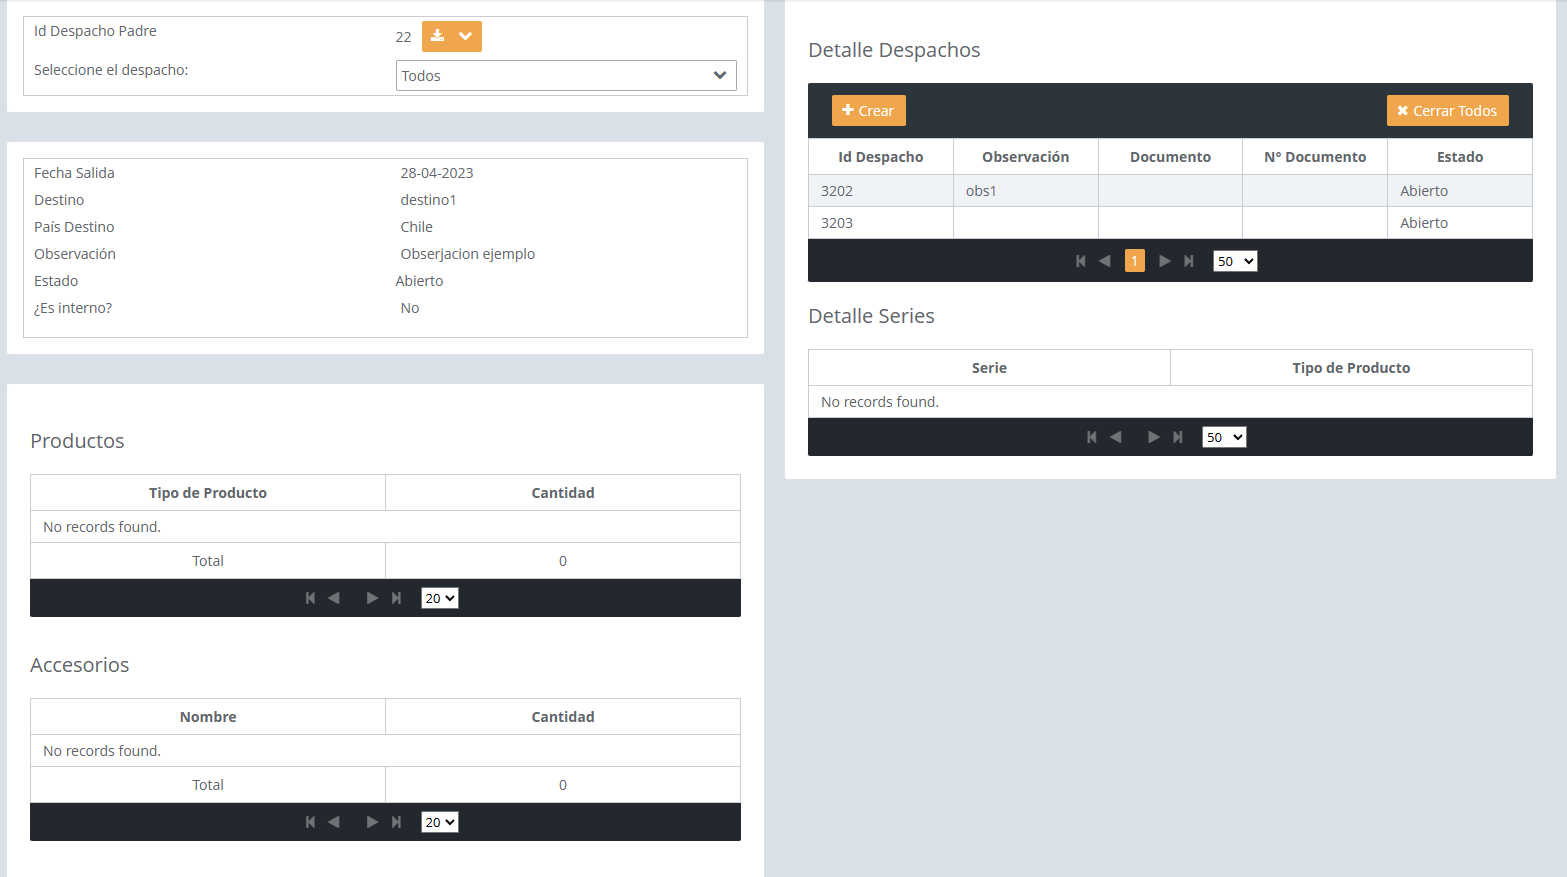
\includegraphics[width=0.5\textwidth]{dm-view}
	\caption{\label{fig:dm-view} Formulario creación despacho múltiple. Fuente: Elaboración propia.}
\end{figure}

\begin{itemize}
    \item Lado izquierdo:
    \begin{itemize}
        \item La primera sección contiene:
        \begin{itemize}
            \item ID del despacho padre, junto a un botón para descargar el reporte del despacho.
            \item Selector de despacho hijo. Al seleccionar la opción 'Todos' se muestra la vista del despacho padre. Si se selecciona la ID de un despacho hijo, se muestra la vista de ese despacho de manera similar a la vista de un despacho individual.
        \end{itemize}
        \item Información del despacho padre. La propiedades son editables.
        \item Tabla de productos: Muestra la cantidad de productos ingresados en todos los despachos hijos.
        \item Tabla de accesorios: Muestra la cantidad de accesorios ingresados en todos los despachos hijos.
    \end{itemize}
    \item Lado derecho:
    \begin{itemize}
        \item Detalle de despachos: Tabla que muestra los despachos hijos. En el \textit{header} de la tabla tiene botónes para crear un nuevo despacho (Se abre un formulario con las propiedades del despacho individual) y para cerrar todos los despachos.
        \item Detalle de series: Tabla que muestra todas las series de los productos ingresados a los despacho hijos.
    \end{itemize}
\end{itemize}

Al seleccionar un despacho hijo, la vista mostrará el despacho seleccionado al igual que en la vista de despacho individual y se podrá editar, agregar productos/accesorios, cerrar/abrir el despacho.

Al editar las propiedades de un despacho múltiple, modificará de igual manera a los despachos hijos. De igual forma, si se editan las propiedades heredadas de un despacho hijo de manera individual, los cambios se modificarán en los demás despachos hijos y el despacho padre.

El estado del despacho padre depende de los despachos hijos, si todos los despachos hijos están cerrados, entonces el despacho padre está cerrado. En el caso de que haya al menos un despacho hijo abierto, el despacho padre aparece abierto. Mismo caso ocurre con la \textit{flag} de despacho interno.

En la vista de despacho individuales, al entrar en un despacho, en la sección de información se agrega un nueva propiedad 'Id Despacho Padre' que, como dice el nombre, indica la ID del despacho padre. Al hacer click sobre este Id redireccionará a la vista del despacho padre en Despacho Múltiples.
Al lado de esta ID, hay un botón que permite desvincular el despacho del despacho padre. 
En el caso que el despacho no pertenezca a un despacho múltiple, se podrá ingresar la ID de un despacho padre para vincularlo a este. Solo se podrá vincular un despacho individual a un despacho múltiple si las propiedades del despacho múltiple coinciden con el despacho individual.

\subsubsubsection{ACTUALIZACIÓN MASIVA DE PRODUCTOS}

El área de producción al hacer el testeo del hardware y si existe un fallo se debe dejar el registro en el historial del producto en \textit{Operations}.
Cada producto tiene asociado un historial, las historias del historial se pueden agregar de forma manual o de forma automática realizando ciertas acciones como agregar un producto a un despacho.
Los tipos de historia que se pueden crear de forma manual son:
\begin{itemize}
    \item Observación.
    \item Fallo PrePorducción.
    \item Fallo PostProducción.
\end{itemize}

Para las historias de fallo, se debe ingresar el tipo de falla.

Debido a que se hacen pruebas a muchos productos, el ir agregando el registro a cada producto de manera individual tomaría mucho tiempo para los trabajadores.

Es por esto que se plantea hacer una nueva herramienta en \textit{Operations} que permita poder hacer una actualización masiva de productos para poder agregar registros al historial de los productos y bloquearlos si es necesario.

Esta nueva herramienta estará en el menú lateral de \textit{Operations} (Figura \ref{fig:history-menu}). Esta herramienta (Figura \ref{fig:history-view}) consta de dos secciones: Tabla de productos y formulario de registro.

\begin{figure}[H]
	\centering
	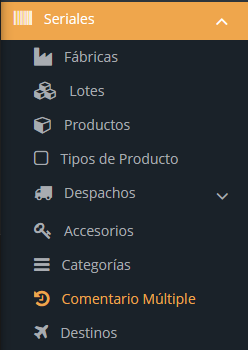
\includegraphics[width=0.5\textwidth]{history-menu}
	\caption{\label{fig:history-menu} Sección de Comentario Múltiple en el menú. Fuente: Elaboración propia.}
\end{figure}

\begin{figure}[H]
	\centering
	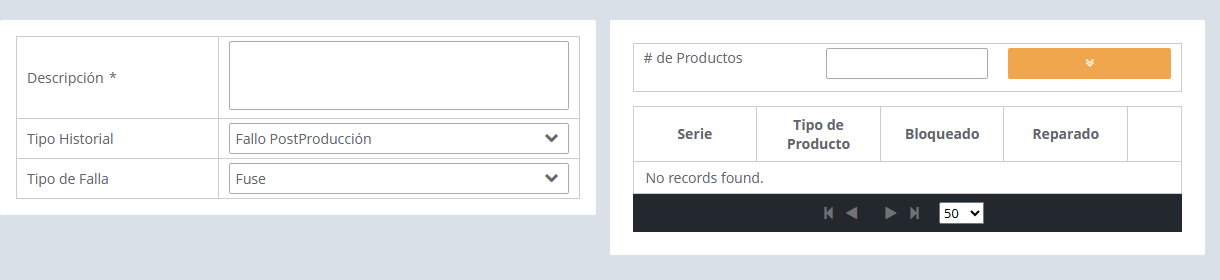
\includegraphics[width=0.5\textwidth]{history-view}
	\caption{\label{fig:history-view} Vista de Comentario Múltiple. Fuente: Elaboración propia.}
\end{figure}

El formulario de registro contiene:
\begin{itemize}
    \item Un \textit{TextArea} para ingresar un comentario.
    \item Selector \textit{dropdown} para el tipo de historia.
    \item En caso de seleccionar un tipo de historia de fallo, se desplegará otro selector \textit{dropdown} para escoger el tipo de fallo.
    \item Botón para guardar los registros.
\end{itemize}

La tabla de productos tendrá lo siguiente:

\begin{itemize}
    \item Un input donde se ingresará la serie del producto a ingresar.
    \item Tabla de productos, que tiene las siguientes columnas:
    \begin{enumerate}
        \item Serie del producto.
        \item Checkbox para (des)bloquear el producto.
        \item Si se escoge tipo de historia de fallo en el formulario, se mostrará un nueva columna para indicar si el producto está reparado o no, con un \textit{checkbox} (Figura \ref{fig:history-view}).
    \end{enumerate}    
\end{itemize}

\begin{figure}[H]
	\centering
	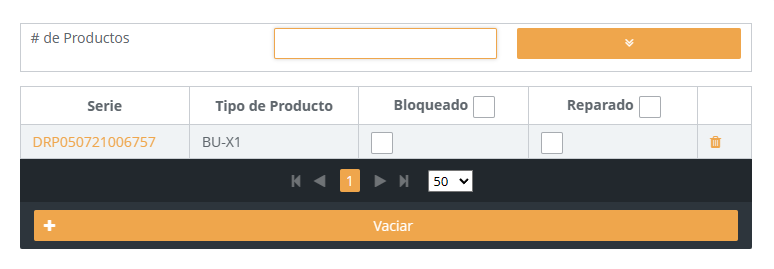
\includegraphics[width=0.5\textwidth]{history-table-1}
	\caption{\label{fig:history-view} Tabla de productos. Fuente: Elaboración propia.}
\end{figure}

Al guardar los registros, si se entra a la vista de alguno de los productos ingresados, se mostrará la historía en la tabla de historial y según como se seleccionó en la tabla mostrará si está bloqueado o no (Figura *).
\iffalse
\subsubsection{CERTIFICADOS TESTBED}

Dentro de las tareas que cumple el área de producción es son las pruebas del hardware, cada prueba queda documentada con
un certificado en donde se indica si el hardware pasó o no las pruebas para seguir con su producción. Estos certificados son
almacenados en un servidor FTP que después se guardan en un bucket de S3.

La aplicación de \textit{Operations} es para la gestión de lotes y despachos de productos, además de la edición de productos.
El producto tiene un historial con historias asociadas que indican ingresos a lotes, despachos, marcar como producto fallado y/o reparado.

Los trabajadores para acceder a los certificados testbed...

Teniendo esto en cuenta, se plantea implementar un modo que agregue al historial del producto testeado un registro junto con el certificado Testbed en \textit{Operations}.

En \textit{Operations}, los productos tienen un historial de movimientos, acciones (creación, ingreso a despacho, etc.), registro de fallos/arreglos, entre otros.
Un registro en el historial contiene el tipo de historia, fecha, usuario y descripción. Dentro de los tipos de historia estan:
\begin{itemize}
    \item Fallo Pre-Producción
    \item Fallo Post-Producción
\end{itemize}

Para solucionar esta problemática, se va a agregar un nuevo tipo de historia llamado 'Certificados Testbed' para registrar los certificados testbed, valga la redundancia, de los productos.
Esta historia se registrará automáticamente cuando el trabajador de taller que esté probando los productos suba los certificados a un servidor FTP. Los certificados en este servidor se respaldan en un \textit{bucket} de S3 en \textit{Amazon Web Services}.
Cada vez que se agregue un certificado al \textit{bucket}, se activa una función \textit{Lambda} que guardará en la base de datos de \textit{Operations} en una nueva tabla creada para los certificados.

Las columnas de la tabla de certificados en la base de datos son las siguientes: 
\begin{itemize}
    \item Fecha.
    \item Llave del objeto en el \textit{bucket}.
    \item Serie del producto.
\end{itemize}
Esta tabla tendrá un \textit{trigger} que se activará el ingresar un nuevo registro, que creará la historia si y solo si el producto está creado en \textit{Operations}.
En el caso que el producto aún no haya sido ingresado en \textit{Operations}, la historia se agregará cuando se cree el producto con un \textit{trigger} en la tabla de productos.
Estas historias no se podrán editar ni eliminar.

En el historial del producto, la historia de certificados mostrará en la descripción un \textit{presigned URL} con el certificado.

Teniendo estas historias de certificados, se agregará una restricción en los despachos, el cuál no se permitirá ingresar un producto que no tenga un certificado testbed.
\fi

\subsubsection{SETUP}

\subsubsubsection{CONFIGURADOR DE FUENTES}

Una de las herramientas más recientes que se ofrece en \textit{DropControl} es el Análisis de Fuentes. En esta herramienta se pueden visualizar las distintas fuentes de agua de un campo como el tranque, canal, equipo de riego e impulsión.
Para mostrar las fuentes de agua en la herramienta, se deben hacer las configuraciones de las fuentes de agua y las conexiones entre ellas en la aplicación de \textit{SETUP}.

Para realizar estas configuraciones se decidió crear un configurador gráfico, donde se agregan 'nodos' a una 'pizarra'. Estos nodos tienen puertos de entrada y salida donde se conectaran con los demás fuentes de agua. Al hacer click sobre sobre estos nodos, se abrirá un formulario donde se agregarán las configuraciones de la respectiva fuente de agua.

Esta configuración tendrá una segunda fase donde luego de guardar los cambios del configurador gráfico, se podrá configurar las coordenadas de las fuentes de agua de forma manual o haciendo click en el mapa.

Este configurador gráfico estará disponible como una configuración en la configuración \textit{Wizard} de \textit{SETUP}, en el paso de `Otras configuraciones` existirá una opción de configuración bajo el nombre `Configuración de fuentes`.
Al seleccionar esta nueva configuración (Figura \ref{fig:water-view}), se mostrará una `pizarra` en el cual se realizará la configuración de fuentes del campo mediante la creación de un diagrama. El diagrama los siguientes elementos (Figura \ref{fig:water-nodes-board}):
\begin{itemize}
    \item \textbf{Metrahidráulicas (Fuentes de agua):} Estos serían los nodos del diagrama. Dentro de las metrahidráulicas disponibles están:
          \begin{itemize}
              \item Canal
              \item Equipo
              \item Impulsión
              \item Tranque
              \item Pozo
          \end{itemize}
    
\end{itemize}

\begin{figure}[H]
	\centering
	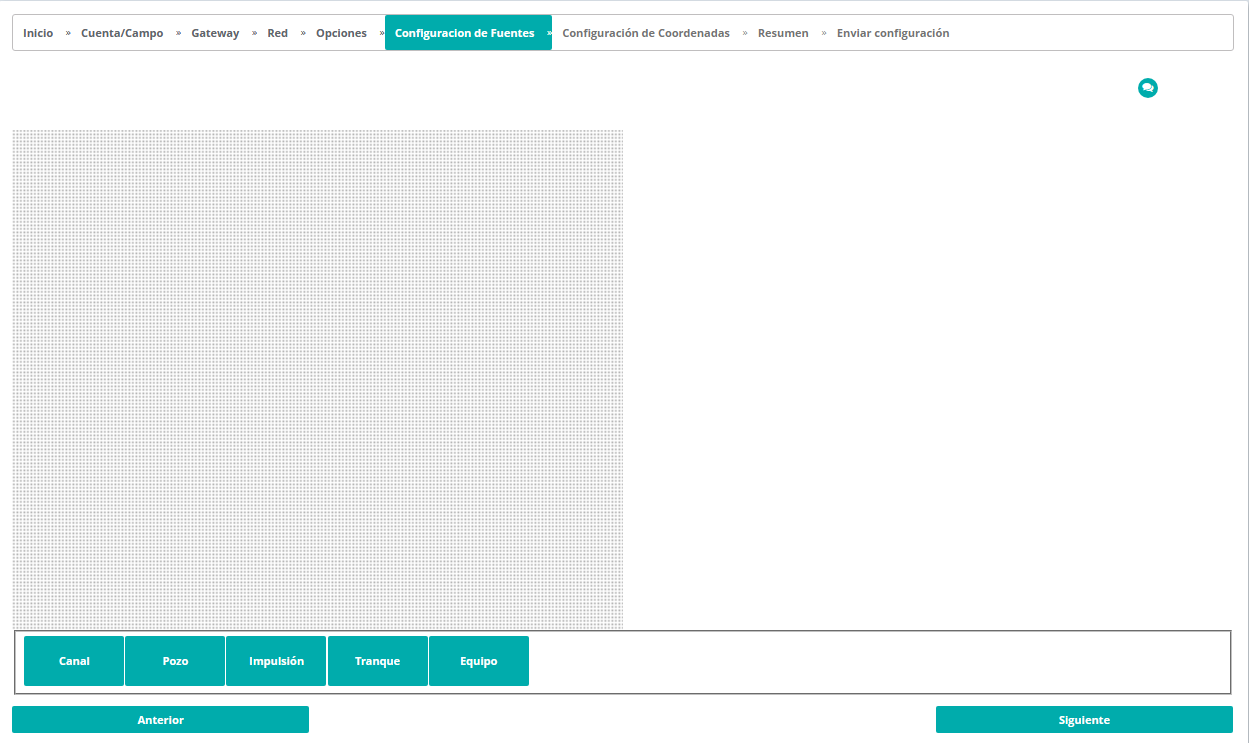
\includegraphics[width=0.5\textwidth]{water-view}
	\caption{\label{fig:water-view} Vista de Configurador de fuentes. Fuente: Elaboración propia.}
\end{figure}

\begin{figure}[H]
	\centering
	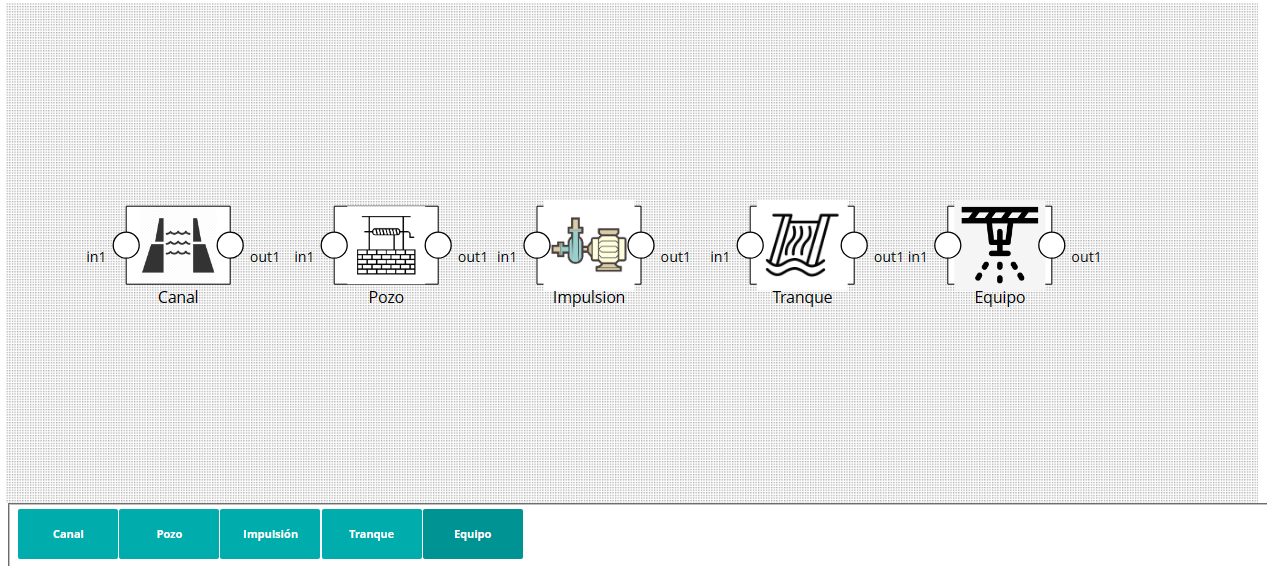
\includegraphics[width=0.5\textwidth]{water-nodes-board}
	\caption{\label{fig:water-nodes-board} Elementos del diagrama. Fuente: Elaboración propia.}
\end{figure}

Las restricciones de conexión se muestran en la figura \ref{fig:water-connections}.

\begin{figure}[H]
	\centering
	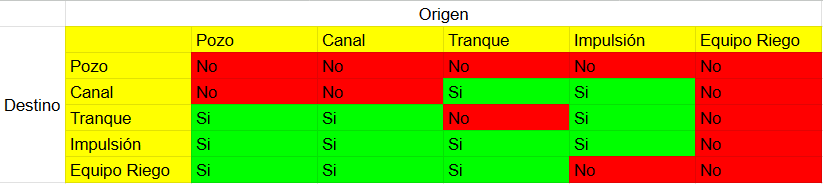
\includegraphics[width=0.5\textwidth]{water-connections}
	\caption{\label{fig:water-connections} Sección de Comentario Múltiple en el menú. Fuente: Elaboración propia.}
\end{figure}

La conexión entre metahidraulica se conoce como 'Conexiones Metrahidráulica'. Esta conexión es la flecha que se muestra en la figura \ref{fig:water-conexion-mh}.

\begin{figure}[H]
	\centering
	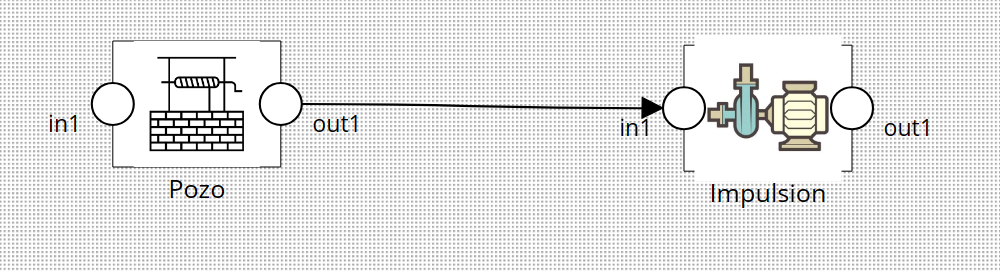
\includegraphics[width=0.5\textwidth]{water-conexion-mh}
	\caption{\label{fig:water-conexion-mh} Conexión Metrahidráulica. Fuente: Elaboración propia.}
\end{figure}

Además de hacer el diagrama, las metrahidráulicas tiene sus propias propiedades, las cuales se pueden asignar haciendo click derecho sobre estos. Al hacer click se abrirá un formulario al lado de la pizarra con las propiedades de la metrahidráulica escogida.
Los formularios de cada elemento:
\begin{itemize}
    \item Canal (Figura \ref{fig:water-canal-form})
    \item Equipo (Figura \ref{fig:water-canal-form})
    \item Impulsión (Figura \ref{fig:water-impulsion-form})
    \item Tranque (Figura \ref{fig:water-tranque-form})
    \item Pozo (Figura \ref{fig:water-pozo-form})
\end{itemize}

\begin{figure}[H]
	\centering
	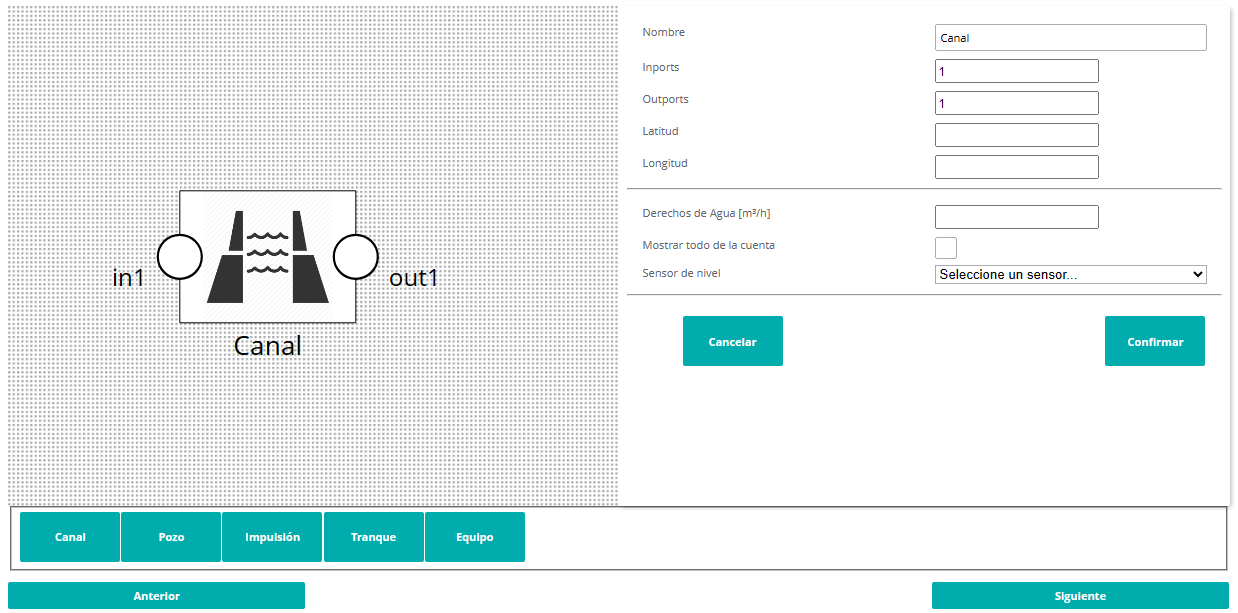
\includegraphics[width=0.5\textwidth]{water-canal-form}
	\caption{\label{fig:water-canal-form} Formulario Canal. Fuente: Elaboración propia.}
\end{figure}

\begin{figure}[H]
	\centering
	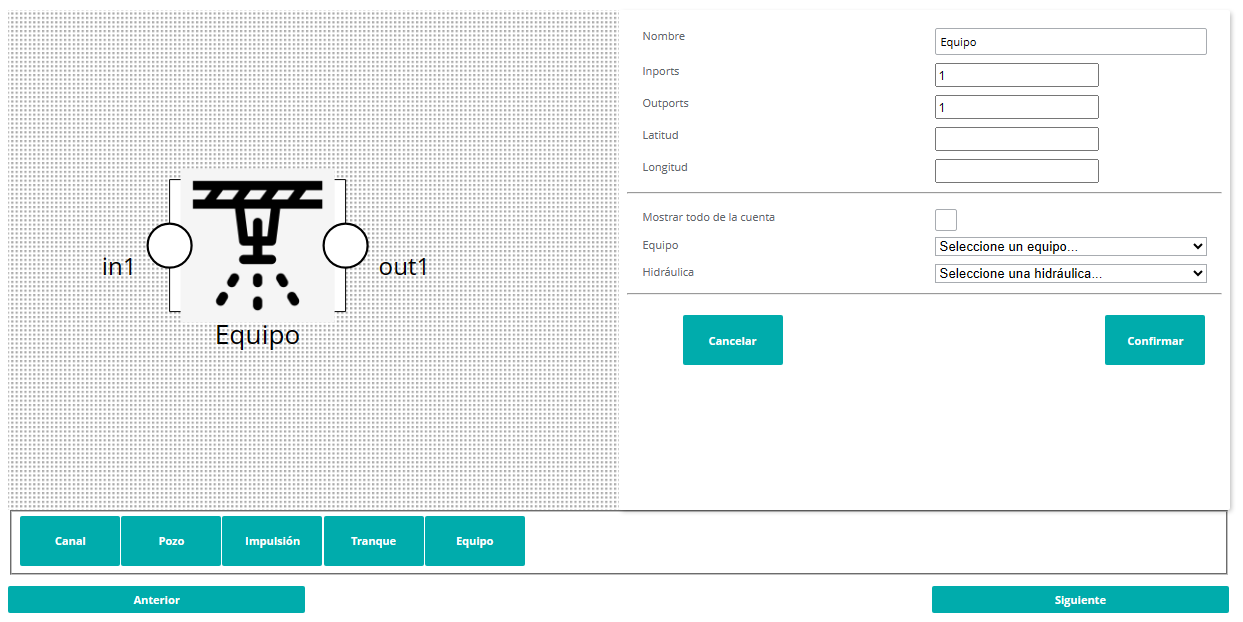
\includegraphics[width=0.5\textwidth]{water-equipo-form}
	\caption{\label{fig:water-Equipo-form} Formulario Equipo. Fuente: Elaboración propia.}
\end{figure}

\begin{figure}[H]
	\centering
	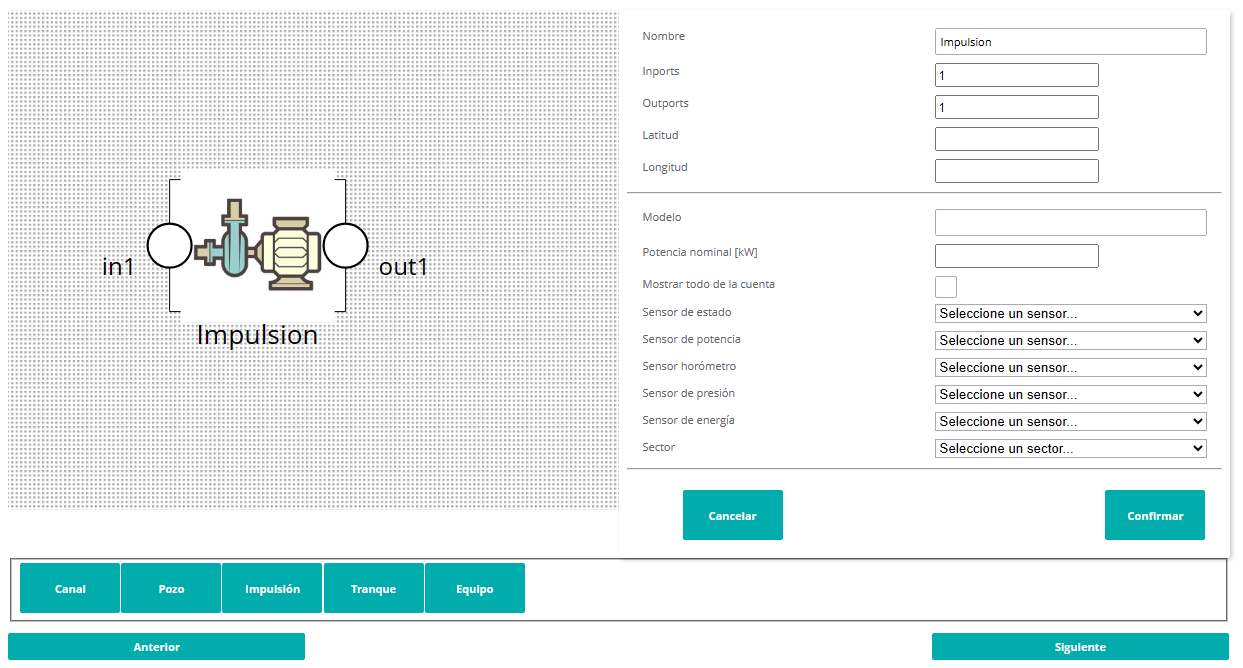
\includegraphics[width=0.5\textwidth]{water-impulsion-form}
	\caption{\label{fig:water-impulsion-form} Formulario Canal. Fuente: Elaboración propia.}
\end{figure}

\begin{figure}[H]
	\centering
	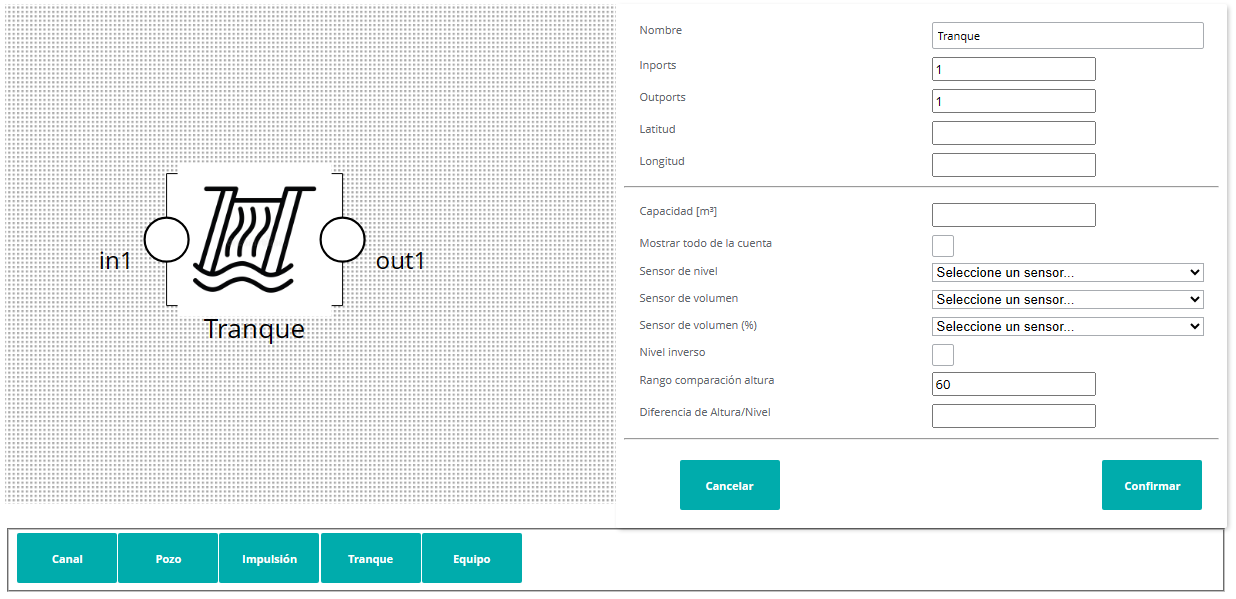
\includegraphics[width=0.5\textwidth]{water-tranque-form}
	\caption{\label{fig:water-tranque-form} Formulario Tranque. Fuente: Elaboración propia.}
\end{figure}

\begin{figure}[H]
	\centering
	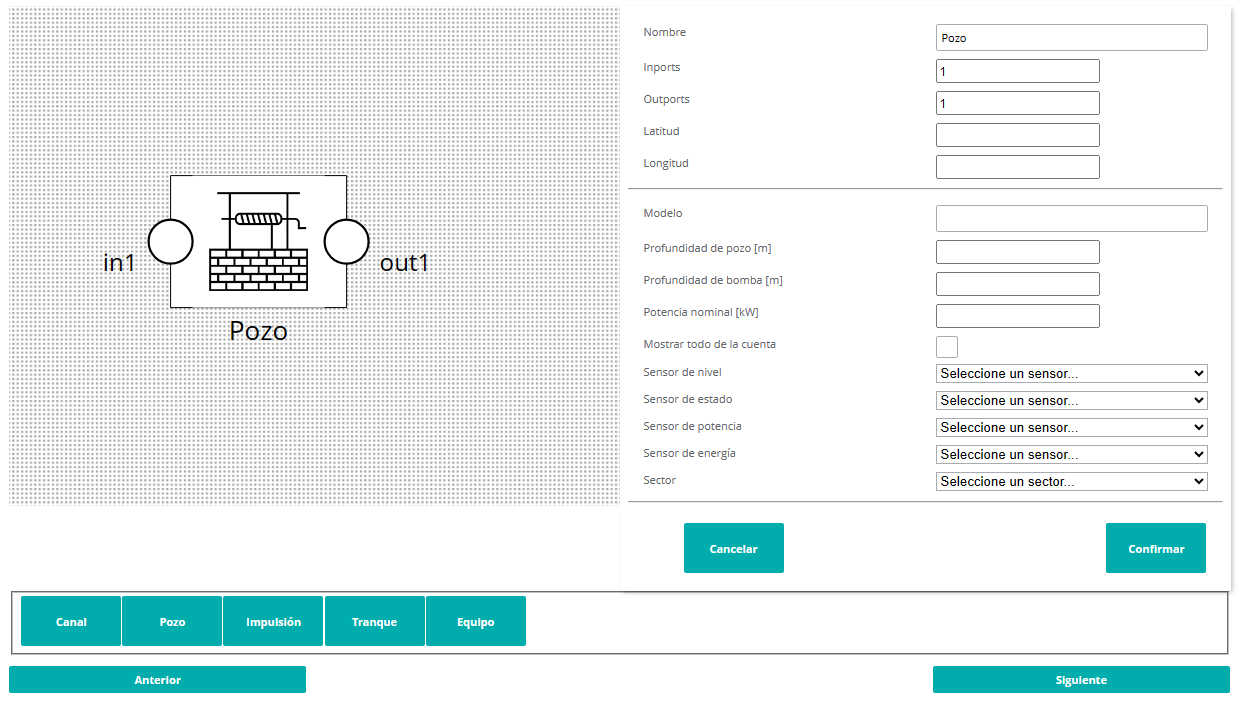
\includegraphics[width=0.5\textwidth]{water-pozo-form}
	\caption{\label{fig:water-pozo-form} Formulario Pozo. Fuente: Elaboración propia.}
\end{figure}

Existen 2 propiedades que está en todos los formularios, los campos de \textit{Inports} y \textit{Outports}. Esta propiedad indica el número de entradas y salidas de la fuente (Figura \ref{fig:water-node-ports}).

\begin{figure}[H]
	\centering
	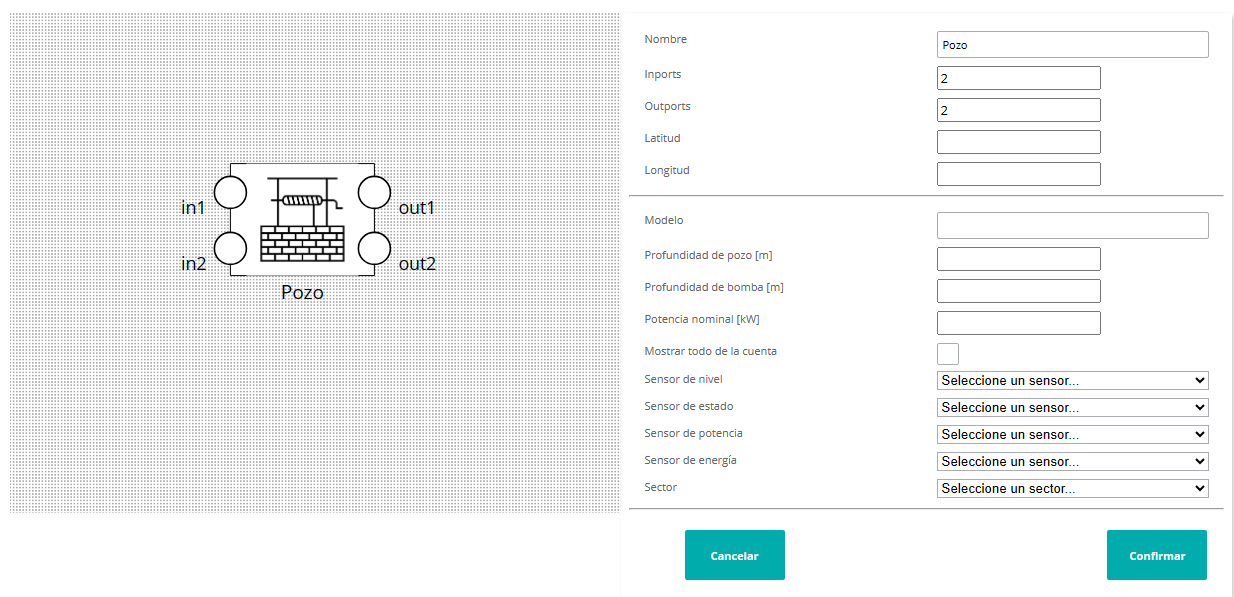
\includegraphics[width=0.5\textwidth]{water-node-ports}
	\caption{\label{fig:water-node-ports} Entradas y salidas de una fuente. Fuente: Elaboración propia.}
\end{figure}

También, las entradas y salidas tienen propiedades al igual que las metrahidráulicas. Haciendo click derecho sobre las entradas/salidas que esten conectadas, aparece un formulario para asignar las propiedades de la entrada/salida de la metahidraulica (Figura \ref{fig:water-conexion-form}).

\begin{figure}[H]
	\centering
	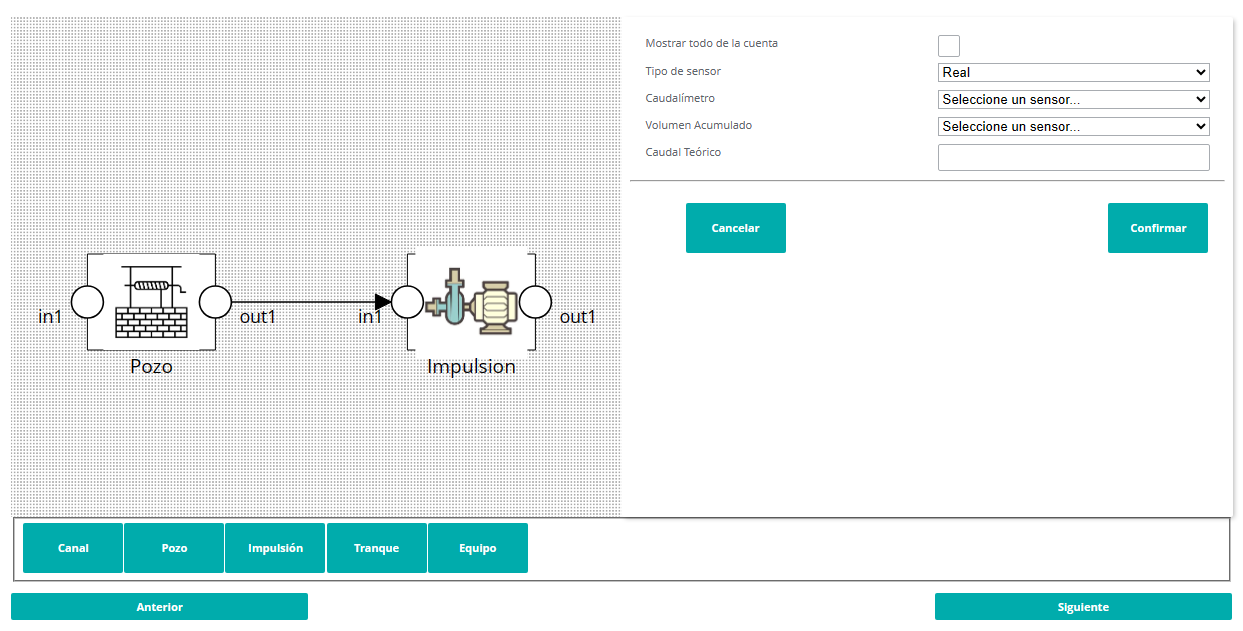
\includegraphics[width=0.5\textwidth]{water-connection-form}
	\caption{\label{fig:water-conexion-form} Formulario Entrada/Salida. Fuente: Elaboración propia.}
\end{figure}

Para poder eliminar ya sea una fuente o conexión, se debe pasar el cursor por sobre el elemento para que aparezca un ícono como se muestran en las figuras \ref{fig:water-delete} y \ref{fig:water-delete-connection}.

\begin{figure}[H]
	\centering
	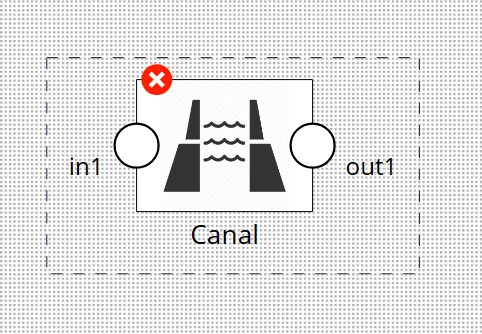
\includegraphics[width=0.5\textwidth]{water-delete}
	\caption{\label{fig:water-delete} Eliminación Fuente. Fuente: Elaboración propia.}
\end{figure}

\begin{figure}[H]
	\centering
	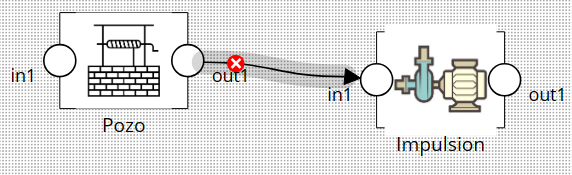
\includegraphics[width=0.5\textwidth]{water-delete-connection}
	\caption{\label{fig:water-delete-connection} Eliminación Conexión Metrahidráulica. Fuente: Elaboración propia.}
\end{figure}

Cuando una entrada/salida tiene un caudalimetro asignado, este tiene un color rojo, como muestra en la figura \ref{fig:water-port-caudal}.

\begin{figure}[H]
	\centering
	\includegraphics[width=0.5\textwidth]{water-port-caudal}
	\caption{\label{fig:water-port-caudal} Asignación caudalimetro en entrada. Fuente: Elaboración propia.}
\end{figure}

Para poder realizar este diagrama, se utilizará la librería de \textit{JavaScript}, \textit{JointJS}\footnote{\href{https://www.jointjs.com/}{JointJS}}. 
Esta libreria permite la creación de diagramas meidante objetos \textit{JSON}, esto nos ayuda a poder crear y cargar diagramas de una forma más sencilla. Además, esta librería soporta atributos \textit{custom}, lo que nos permite poder guardar los datos de los formularios en los \textit{json} de los elementos.
Otro beneficio de esta librería, es la facilidad del trabajo con las entradas y salidas de las fuentes (\textit{ports}\footnote{\href{https://resources.jointjs.com/tutorial/ports}{JointJS: Working with Ports}}) para poder agregar/eliminar \textit{ports}, asignar las propiedades del formulario.

Al guardar los cambios se entrará a otra configuración para asignar las coordenadas de las metrahidráulicas.
En esta configuración se tiene un mapa junto a una tabla de las fuentes (Figura \ref{fig:water-map-view}). La tabla tiene las siguientes columnas:
\begin{enumerate}
    \item Fuente de agua.
    \item Coordenadas.
    \item Acciones (Figura \ref{fig:water-table-actions}):
          \begin{itemize}
            \item Editar.
            \item Crear
            \item Eliminar coordenada.
            \item Centrar en mapa.
          \end{itemize}
\end{enumerate}

\begin{figure}[H]
	\centering
	\includegraphics[width=0.5\textwidth]{water-map-view}
	\caption{\label{fig:water-map-view} Configuración de Coordenadas. Fuente: Elaboración propia.}
\end{figure}

\begin{figure}[H]
	\centering
	\includegraphics[width=0.5\textwidth]{water-table-actions}
	\caption{\label{fig:water-table-actions} Configuración de Coordenadas: Acciones. Fuente: Elaboración propia.}
\end{figure}

Para ingresar las coordenadas de cada fuente, se pueden hacer de dos formas:
\begin{itemize}
    \item Al hacer click en la acción de editar, la fila permitirá editar el nombre de la fuente ye ingresar las coordenadas de forma manual, vease figura \ref{fig:water-map-edit}.    
    \item Al hacer click en la acción crear, se mostrará un tooltip que indica que se tiene que hacer click en un lugar del mapa. Al seleccionar el lugar en el mapa se agregará un punto en el mapa y se asignarán las coordenadas a la fuente (Figura \ref{fig:water-map-create}).
\end{itemize}

 \begin{figure}[H]
	\centering
	\includegraphics[width=0.5\textwidth]{water-map-edit}
	\caption{\label{fig:water-map-edit} Acción editar. Fuente: Elaboración propia.}
\end{figure}

\begin{figure}[H]
   \centering
   \includegraphics[width=0.5\textwidth]{water-map-create}
   \caption{\label{fig:water-map-create} Acción crear. Fuente: Elaboración propia.}
\end{figure}

Al tener las coordenadas asignadas a cada fuente, hacer click en siguiente para guardar.

\subsection{ENTORNO DE TRABAJO}

\subsubsection{STACK DE TECNOLOGÍAS}

Para el desarrollo en las distintas aplicaciones se tienen los correspondientes \textit{stack} de tecnologías.

\begin{itemize}
    \item \textbf{\textit{Admin} de \textit{DropControl}}
    \begin{itemize}
        \item Framework: \textit{React.js}
        \item IDE: VS Code
        \item Base de Datos: \textit{PostgreSQL}
        \item Hosting: \textit{AWS Amplify}
    \end{itemize}
    \item \textbf{\textit{Operations}}
    \begin{itemize}
        \item Framework: JavaServer Faces, Primefaces
        \item IDE: Eclipse
        \item Base de Datos: \textit{MySQL}
        \item Hosting: \textit{AWS EC2}
    \end{itemize}
    \item \textbf{\textit{SETUP}}
    \begin{itemize}
        \item Framework: JavaServer Faces, Primefaces
        \item IDE: Eclipse
        \item Base de Datos: \textit{PostgreSQL}
        \item Hosting: \textit{AWS EC2}
    \end{itemize}
\end{itemize}

\iffalse
Los servicios de WiseConn corren en la nube de \textit{Amazon Web Services}, utilizando los distintos servicios que este ofrece para las bases de datos, \textit{backend} y \textit{hosting}. En las siguientes secciones se explicará el entorno de trabajo de cada aplicación.

\subsubsection{OPERATIONS}

\textit{Operations} es una aplicación interna usada por el área de producción de WiseConn para la gestión de inventario, lotes y despachos.

Es una aplicación monolítica, por lo que, el \textit{backend} y \textit{frontend} se desarrollan juntos en el mismo código. La aplicación está desarrollada en JAVA con \textit{JavaServer Faces}, utilizando el \textit{framework} de \textit{PrimeFaces} y se conecta a una base de datos \textit{MySQL}. \textit{Operations} corre en una instancia \textit{EC2}, mientras que, la base de datos .\

\subsubsection{SETUP}

\textit{SETUP} es una aplicación interna para la configuración de cuentas, campos, sectores, usuarios, entre otros. Utilizado principalmente por el área de soporte de WiseConn.

Es una aplicación monolítica desarrollada en JAVA con \textit{JavaServer Faces}, utilizando el \textit{framework} de \textit{PrimeFaces} y se conecta a la base de datos \textit{PostgreSQL} de \textit{DropControl}.

\subsubsection{ADMIN DE DROPCONTROL}

La aplicación de \textit{Admin} es utilizada por los usuarios administradores de campo para la configuración de campos, sectores, red de nodos, etc.

\textit{Admin} es una aplicación destribuida, es decir, el \textit{backend} y \textit{frontend} están separadas.

Para desplegar la aplicación se utiliza el servicio de \textit{AWS Amplify}, este servicio se encarga de crear/actualizar los recursos del \textit{backend} y de desplegar la aplicación web.

Para el \textit{frontend} se utiliza el framework de \textit{JavaScript}, \textit{React.js}. Además, se utilizan componentes de \textit{Syncfusion}\footnote{\href{https://www.syncfusion.com/react-components}{Syncfusion React Components}}.

Respecto al \textit{backend}, este es \textit{serverless}. Se utilizan funciones \textit{Lambda} con el lenguaje de \textit{JavaScript} que se conectan a una base de datos \textit{PostgreSQL}.
\fi
\newpage
\secnumbersection{VALIDACIÓN DE LA SOLUCIÓN}

En la presente sección se presentarán las pruebas que validan los requerimientos de las herramientas/funcionalidades desarrolladas para las distintas aplicaciones de WiseConn.

\subsection{ADMIN DE DROPCONTROL}

\subsubsection{CONFIGURADOR DE MAPA}

\subsubsubsection{FUNCIONAMIENTO}

Para poder entrar a esta herramienta se debe dirigir al \textit{Dashboard de campo} de \textit{Admin}, y en la sección de mapa hacer click sobre el ícono que muestra la figura \ref{fig:mapcfg-1}.

\begin{figure}[H]
	\centering
	\includegraphics[width=0.8\textwidth]{mapcfg-1}
	\caption{\label{fig:mapcfg-1} Como ingresar al configurador de mapa}
\end{figure}

Al ingresar a esta herramienta, el usuario se encontrará con 2 secciones como se muestra en la figura \ref{fig:mapcfg-2}, teniendo a la izquierda la tabla de sectores y nodos y a la derecha el mapa.

\begin{figure}[H]
	\centering
	\includegraphics[width=0.8\textwidth]{mapcfg-2}
	\caption{\label{fig:mapcfg-2} Configurador de mapa}
\end{figure}

En la tabla, para cambiar entre sectores y nodos se debe hacer click en los botones de la esquina superior izquierda de la tabla.

\begin{figure}[H]
	\centering
	\includegraphics[width=0.8\textwidth]{mapcfg-tables}
	\caption{\label{fig:mapcfg-tables} Tabla de nodos y sectores}
\end{figure}

El mapa mostrará sectores o nodos según la tabla seleccionada como se ve en la figura \ref{fig:mapcfg-maps}. El primer mapa muestra los sectores representados por polígonos, mientras que, el segundo mapa muestra los nodos representados por marcadores. Como muestra en la figura, los sectores ya asignados son polígonos verdes y los nodos tienen un ícono según su tipo.

\begin{figure}[H]
	\centering
	\includegraphics[width=0.8\textwidth]{mapcfg-maps}
	\caption{\label{fig:mapcfg-maps} Tabla de nodos y sectores}
\end{figure}

Para cargar el archivo que contiene nuestros sectores y/o nodos, se debe hacer click sobre el botón de 'Cargar Archivo', como se muestra en la figura \ref{fig:mapcfg-load-file}

\begin{figure}[H]
	\centering
	\includegraphics[width=0.8\textwidth]{mapcfg-load-file}
	\caption{\label{fig:mapcfg-load-file} Carga de archivo .kmz}
\end{figure}

Al cargar el archivo .kmz, en las tablas se agrega una columna en medio con un selector como se aprecia en la figura \ref{fig:mapcfg-tables-edit}

\begin{figure}[H]
	\centering
	\includegraphics[width=0.8\textwidth]{mapcfg-tables-edit}
	\caption{\label{fig:mapcfg-tables-edit} Tablas de sectores y nodos al cargar un archivo.}
\end{figure}

En el mapa se agregan los polígonos del archivo con un color celeste (figura \ref{fig:mapcfg-cfg-map-zone}), mientras que los marcadores se muestran con un punto con un borde negro y centro azul (figura \ref{fig:mapcfg-cfg-map-node}).

\begin{figure}[H]
	\centering
	\includegraphics[width=0.8\textwidth]{mapcfg-cfg-map-zone}
	\caption{\label{fig:mapcfg-cfg-map-zone} Tablas de sectores y nodos al cargar un archivo.}
\end{figure}

\begin{figure}[H]
	\centering
	\includegraphics[width=0.8\textwidth]{mapcfg-cfg-map-node}
	\caption{\label{fig:mapcfg-cfg-map-node} Tablas de sectores y nodos al cargar un archivo.}
\end{figure}

\subsubsubsection{DATOS}

En el año 2023, como muestra la figura \ref{fig:mapcfg-analytics-view} el configurador de mapa tuvo 769 vistas, con un total de 187 usuarios y con una retención de aproximadamente 3 minutos.
\begin{figure}[H]
	\centering
	\includegraphics[width=0.8\textwidth]{mapcfg-analytics-view}
	\caption{\label{fig:mapcfg-analytics-view} Datos de vistas de la herramienta de configurador de mapa en el año 2023.}
\end{figure}
\iffalse
\subsubsection{GRAFICADOR LIBRE}

\subsubsubsection{FUNCIONAMIENTO}

Esta nueva herramienta implementada en la aplicación de \textit{Admin de DropControl} se encuentra en el menú lateral como muestra en la figura \ref{fig:menu-admin-graf}

\begin{figure}[H]
	\centering
	\includegraphics[width=0.5\textwidth]{menu-admin-graficador}
	\caption{\label{fig:menu-admin-graf} Graficador Libre en el menú de \textit{Admin}}
\end{figure}

En la herramienta se encontrará con 4 secciones, como se muestra en la figura \ref{fig:graf1}:
\begin{enumerate}
    \item Selección de nodo/sensores.
    \item Selección de rango de fechas.
    \item Gráfico.
    \item Tabla de datos.
\end{enumerate}

\begin{figure}[H]
	\centering
	\includegraphics[width=0.8\textwidth]{graficador-1}
	\caption{\label{fig:graf1} Secciones del graficador libre}
\end{figure}

El primer paso es escoger los sensores que queremos visualizar en el gráfico, en la primera sección selecciones en el primer selector el nodo seguido del sensor y opcionalmente el color (figura \ref{fig:grafselect}).

\begin{figure}[H]
	\centering
	\includegraphics[width=0.8\textwidth]{graf-select}
	\caption{\label{fig:grafselect} Selección de sensor}
\end{figure}

Para escoger otro sensor se puede hacer agregando otra fila vacía haciendo click en el botón 'Agregar' (figura \ref{fig:graf-add-row-1}) y repitiendo el paso anterior.

\begin{figure}[H]
	\centering
	\includegraphics[width=0.8\textwidth]{graf-add-row-1}
	\caption{\label{fig:graf-add-row-1} Agregar una nueva fila vacía}
\end{figure}

Otra forma de agregar sensores es con los botones con el símbolo '+' presente en las filas. El primer botón agrega una nueva fila con el siguiente nodo seleccionado junto al sensor del mismo tipo (figura \ref{fig:graf-add-row-2}), mientras que el segundo botón agrega una nueva fila con el mismo nodo seleccionado pero con el siguiente sensor en la lista (figura \ref{fig:graf-add-row-3}).

\begin{figure}[H]
	\centering
	\includegraphics[width=0.8\textwidth]{graf-add-row-2}
	\caption{\label{fig:graf-add-row-2} Agregar una nueva fila con el siguiente nodo}
\end{figure}

\begin{figure}[H]
	\centering
	\includegraphics[width=0.8\textwidth]{graf-add-row-3}
	\caption{\label{fig:graf-add-row-3} Agregar una nueva fila con el siguiente sensor del nodo}
\end{figure}

Para eliminar una fila se debe hacer click en el último botón de la fila, con símbolo de basura (figura \ref{fig:graf-delete-row}).

\begin{figure}[H]
	\centering
	\includegraphics[width=0.8\textwidth]{graf-delete-row}
	\caption{\label{fig:graf-delete-row} Agregar una nueva fila con el siguiente sensor del nodo}
\end{figure}

El siguiente paso es escoger el rango de fechas de los datos, como se muestra en la figura \ref{fig:graf-date-range-1}.

\begin{figure}[H]
	\centering
	\includegraphics[width=0.8\textwidth]{graf-date-range-1}
	\caption{\label{fig:graf-date-range-1} Selección de rango de fechas}
\end{figure}

Se puede escoger un rango personalizado, como se mostró anteriormente, o escoger rangos predeterminados como muestra en la figura \ref{fig:graf-date-range-2}.

\begin{figure}[H]
	\centering
	\includegraphics[width=0.8\textwidth]{graf-date-range-2}
	\caption{\label{fig:graf-date-range-2} Selección de rango de fechas}
\end{figure}

Luego de tener el rango de fechas seleccionado, hacer click en el botón 'ver' para mostrar los datos de los sensores seleccionados (figura \ref{fig:graf-display-1})

\begin{figure}[H]
	\centering
	\includegraphics[width=0.8\textwidth]{graf-display-1}
	\caption{\label{fig:graf-display-1} Gráfico}
\end{figure}

En la última sección se encuentra la tabla de datos del gráfico, en donde se muestran los datos de los sensores donde la primera columna es la fecha y hora del dato y las columnas siguientes son los sensores escogidos con el formato de nombre \{Nodo\}-\{Sensor\} [unidad] (figura \ref{fig:graf-table-1}). 
Además, tiene la funcionalidad de exportar la tabla en formato .xlsx haciendo click en el ícono de descarga en la esquina superior derecha de la tabla.

\begin{figure}[H]
	\centering
	\includegraphics[width=0.8\textwidth]{graf-table-1}
	\caption{\label{fig:graf-table-1} Gráfico}
\end{figure}


\subsubsection{DATOS}

En el año 2023, como muestra la figura \ref{fig:graf-analytics-view} el configurador de mapa tuvo 2947 vistas, con un total de 533 usuarios y con una retención de aproximadamente 1 minuto.
\begin{figure}[H]
	\centering
	\includegraphics[width=0.8\textwidth]{graf-analytics-view}
	\caption{\label{fig:graf-analytics-view} Datos de vistas de la herramienta de graficador libre en el año 2023.}
\end{figure}
\fi

\subsection{OPERATIONS}

\subsubsection{DESPACHOS MÚLTIPLES}

Entrando a la herramienta de \textit{Operations}, en el menú lateral, abrir la sección de Despachos y se encuentran las opciones de 'Individuales' y 'Múltiples' (Figura \ref{fig:op-menu}).

\begin{figure}[H]
	\centering
	\includegraphics[width=1\textwidth]{validation-op-dm/menu.png}
	\caption{\label{fig:op-menu} Menu de Despachos en \textit{Operations}}
\end{figure}

Al hacer click en 'Múltiples' se ingresa a la sección de despachos múltiples (Figura \ref{fig:op-list}).
Se tiene una tabla con los despachos múltiples creados.

\begin{figure}[H]
	\centering
	\includegraphics[width=0.8\textwidth]{validation-op-dm/list.png}
	\caption{\label{fig:op-list} Menu de Despachos en \textit{Operations}}
\end{figure}

Para crear un despacho múltiple se debe hacer click en el botón 'Crear' en la tabla. Al hacer click, se abrirá el formulario de la figura \ref{fig:op-form-create-1}.
Los parámetros previos al 'Número de despachos' son los parámetros del despacho padre, el cual los despachos hijos herederan.

\begin{figure}[H]
	\centering
	\includegraphics[width=1\textwidth]{validation-op-dm/form-create-1.png}
	\caption{\label{fig:op-form-create-1} Formulario de creación de Despacho Múltiple}
\end{figure}

El parámetros 'Número de despachos' indica, valga la redundancia, el número de despachos hijos. Esto se aprecia al comparar la figura \ref{fig:op-form-create-1} y la figura \ref{fig:op-form-create-2}.

\begin{figure}[H]
	\centering
	\includegraphics[width=1\textwidth]{validation-op-dm/form-create-2.png}
	\caption{\label{fig:op-form-create-2} Formulario de creación de Despacho Múltiple con 3 despachos}
\end{figure}

\subsubsection{ACTUALIZACIÓN MASIVA DE PRODUCTOS}

En el menú lateral, la funcionalidad se encuentra bajo el nombre de 'Comentario múltiple' (figura \ref{fig:op-menu-cm}).

\begin{figure}[H]
	\centering
	\includegraphics[width=1\textwidth]{validation-op-cm/menu.png}
	\caption{\label{fig:op-menu-cm} Comentario Múltiple en menú}
\end{figure}

Al ingresar a la funcionalidad, en la sección izquierda se encuentra formulario para ingresar el comentario, mientras que, en la sección derecha se encuentra la tabla de productos al que se le asignará el comentario (figura \ref{fig:op-view-cm}).

\begin{figure}[H]
	\centering
	\includegraphics[width=1\textwidth]{validation-op-cm/view.png}
	\caption{\label{fig:op-view-cm} Comentario Múltiple}
\end{figure}

En la tabla de productos se ingresan las series de productos a los cuales se quiere registrar una historia (figura \ref{fig:op-add-product-cm}).

\begin{figure}[H]
	\centering
	\includegraphics[width=1\textwidth]{validation-op-cm/add-product.png}
	\caption{\label{fig:op-add-product-cm} Comentario Múltiple: Agregar productos}
\end{figure}

En el formulario, si se selecciona el tipo de historial 'Fallo PreProducción' o 'Fallo PostProducción' se muestra un nuevo selector para ingresar el tipo de falla (figura \ref{fig:op-select-history-type-cm}). Estos tipos de historia también afecta la tabla de productos, agregando una nueva columna de tipo \textit{checkbox} para indicar si el producto esta reparado o no (figura \ref{fig:op-tabla-productos-reparado-col-cm}).

\begin{figure}[H]
	\centering
	\includegraphics[width=1\textwidth]{validation-op-cm/select-history-type.png}
	\caption{\label{fig:op-select-history-type-cm} Comentario Múltiple: Tipos de historia}
\end{figure}

\begin{figure}[H]
	\centering
	\includegraphics[width=1\textwidth]{validation-op-cm/tabla-productos-reparado-col.png}
	\caption{\label{fig:op-tabla-productos-reparado-col-cm} Comentario Múltiple: Tabla productos - Columna reparado}
\end{figure}

En la figura \ref{fig:op-test-1-cm} se ve el formulario completo. Al hacer click en guardar se mostrará un diálogo de confirmación (figura \ref{fig:op-test-1-confirm-cm}). Cuando se confirmen los cambios, se agregarán las historias a los productos correspondientes y se muestra un \textit{toast} que confirma el guardado (figura \ref{fig:op-test-1-finish-cm}).

\begin{figure}[H]
	\centering
	\includegraphics[width=1\textwidth]{validation-op-cm/test-1.png}
	\caption{\label{fig:op-test-1-cm} Comentario Múltiple: Formulario completo.}
\end{figure}

\begin{figure}[H]
	\centering
	\includegraphics[width=1\textwidth]{validation-op-cm/test-1-confirm.png}
	\caption{\label{fig:op-test-1-confirm-cm} Comentario Múltiple: Confirmar cambios.}
\end{figure}

\begin{figure}[H]
	\centering
	\includegraphics[width=1\textwidth]{validation-op-cm/test-1-finish.png}
	\caption{\label{fig:op-test-1-finish-cm} Comentario Múltiple: Historias registradas.}
\end{figure}

Los cambios reflejados en los productos se muestra en la figura \ref{fig:op-test-1-products-cm}, en la tabla de historias se encuentra la historia que se agregó, junto a si se marcó como reparada o no, y en la información del producto si este se marcó como bloqueado.

\begin{figure}[H]
	\centering
	\includegraphics[width=1\textwidth]{validation-op-cm/test-1-products.png}
	\caption{\label{fig:op-test-1-products-cm} Comentario Múltiple: Productos después del registro de historias.}
\end{figure}

\subsection{DROPCONTROL}

\subsubsection{FÓRMULAS}

Primero se debe acceder a la herramienta de \textbf{Dashboard Libre} en el menú del nuevo \textbf{DropControl} como muestra en en la figura \ref{fig:dash-libre-menu}.

\begin{figure}[H]
	\centering
	\includegraphics[width=1\textwidth]{widget-formulas/dashboard-libre-menu}
	\caption{\label{fig:dash-libre-menu} \textbf{Dashboard Libre} en el nuevo \textbf{DropControl}. Fuente: Elaboración propia.}
\end{figure}

Seleccionar o crear un \textit{dashboard}. Entrar al modo edición en la esquina superior derecha como muestra en la figura \ref{fig:entrar-modo-edicion}.
\iffalse foto con paso de como entrar al modo edicion \fi
\begin{figure}[H]
	\centering
	\includegraphics[width=1\textwidth]{widget-formulas/entrar-modo-edicion.png}
	\caption{\label{fig:entrar-modo-edicion} Entrar a modo edición. Elaboración propia.}
\end{figure}

Al estar en modo edición, para acceder a los formularios de \textit{widget} de tabla y/o gráfico existen 2 opciones:
\begin{itemize}
	\item Crear un nuevo \textit{widget} haciendo clic en el botón 'Crear...' en la esquina superior derecha (figura \ref{fig:opciones-crear}).
	\item Editar un \textit{widget} existente haciendo clic en el ícono de lápiz en la parte superior del \textit{widget} (figura \ref{fig:editar-widget}).
\end{itemize}
\iffalse pasos para ingresar al formulario de ambas formas \fi
\begin{figure}[H]
	\centering
	\includegraphics[width=1\textwidth]{widget-formulas/opciones-crear.png}
	\caption{\label{fig:opciones-crear} Crear \textit{widget} nuevo. Elaboración propia.}
\end{figure}
\begin{figure}[H]
	\centering
	\includegraphics[width=1\textwidth]{widget-formulas/editar-widget.png}
	\caption{\label{fig:editar-widget} Editar \textit{widget} existente. Elaboración propia.}
\end{figure}

Se utilizará el formulario de gráfico para el paso a paso. Para este caso tenemos una variable de temperatura en unidad \textit{Fahrenheit} el cual vamos a convertir a \textit{Celsius}.
Al entrar al formulario del \textit{widget} entramos a la pestaña de fórmulas (figura \ref{fig:pestana-formulas}).
\iffalse ingresar a formulas \fi
\begin{figure}[H]
	\centering
	\includegraphics[width=1\textwidth]{widget-formulas/pestana-formulas.png}
	\caption{\label{fig:pestana-formulas} Editar \textit{widget} existente. Elaboración propia.}
\end{figure}
Primero rellenamos y seleccionamos todos los \textit{inputs} y dejamos el \textit{input} de fórmula para el final. Como muestra la figura \ref{fig:primer-relleno-formula}, la fórmula tendrá:
\begin{itemize}
	\item Nombre: \textbf{\textit{Celsius}}.
	\item Unidad: ºC
	\item \# Decimales: 3.
	\item Color: Rojo
	\item Tipo: Línea.
	\item Posición de eje: Derecha.
\end{itemize}
\iffalse relleno de inputs \fi
\begin{figure}[H]
	\centering
	\includegraphics[width=1\textwidth]{widget-formulas/primer-relleno-formula.png}
	\caption{\label{fig:primer-relleno-formula} Relleno de \textit{inputs}. Elaboración propia.}
\end{figure}

Se puede ingresar la fórmula completamente a mano o con el botón al lado del \textit{input}. En la figura \ref{fig:lista-boton} muestra la lista al hacer clic en el botón a lado del \textit{input} de formula.
\iffalse lista de boton \fi
\begin{figure}[H]
	\centering
	\includegraphics[width=1\textwidth]{widget-formulas/lista-boton.png}
	\caption{\label{fig:lista-boton} Lista al hacer clic en el botón a lado del \textit{input} de formula. Elaboración propia.}
\end{figure}

Se ingresa la fórmula para convertir desde \textit{Fahrenheit} a \textit{Celsius} (figura \ref{fig:formula-ingresada}).
\iffalse formula \fi
\begin{figure}[H]
	\centering
	\includegraphics[width=1\textwidth]{widget-formulas/formula-ingresada.png}
	\caption{\label{fig:formula-ingresada} Formula de conversión de Fahrenheit a Celsius ingresada en el formulario. Elaboración propia.}
\end{figure}

Hacemos clic en el botón \textbf{Previsualizar}, esperamos a que muestre el gráfico en la parte superior del formulario, tomamos un punto como muestra en la figura \ref{fig:formula-preview} y comparamos un punto.
\iffalse formula previsualizada \fi
\iffalse formula con punto seleccionado \fi
\begin{figure}[H]
	\centering
	\includegraphics[width=1\textwidth]{widget-formulas/formula-preview.png}
	\caption{\label{fig:formula-preview} Previsualización de fórmula en el gráfico. Elaboración propia.}
\end{figure}


\iffalse agregar referencia a formulas \fi

Dentro de las validaciones del formularios están:
\begin{itemize}
    \item Debe contener solo caracteres válidos, es decir, la formula debe contener (figura ...): 
        \SubItem{Números. Si son números decimales se debe usar separador de decimales ya sea punto o coma. Los números no deben contener separados de miles.} 
        \SubItem{Operadores matemáticos: '+' (suma), '-' (resta), '*' (multiplicación), '/' (división) y '\^{}' (potencia).}
        \SubItem{Paréntesis.}
        \SubItem{Funciones soportadas.}
    \item La fórmula debe tener al menos una variable o referencia a una fórmula (figura ...).
    \item No pueden existir referencias circulares al hacer referencias a otras fórmulas (figura ...).
    \item Las variables y fórmulas referenciadas en la fórmula deben existir en el \textit{widget} (figura ...).        
\end{itemize}
\iffalse
\subsection{SETUP}

\subsubsection{CONFIGURADOR DE FUENTES}

En el configurador \textit{Wizard} de \textit{Setup}, al llegar al paso 'Opciones' se encuentran distintas configuraciones que se pueden realizar, dentro de estas se encuentra 'Configuración de Fuentas' como muestra en la figura \ref{fig:ws-wizard-option}

\begin{figure}[H]
	\centering
	\includegraphics[width=1\textwidth]{validation-watersources/wizard-option.png}
	\caption{\label{fig:ws-wizard-option} Configuración de Fuentes en el asistente de configuración \textit{Wizard}}
\end{figure}

Al seleccionar la opción de 'Configuración de Fuentes' y hacer click en siguiente, se redirige a la herramienta.

\begin{figure}[H]
	\centering
	\includegraphics[width=0.8\textwidth]{water-view}
	\caption{\label{fig:water-view} Configurador de fuentes. Fuente: Elaboración propia.}
\end{figure}

A continuación se mostrarán las conexiones permitidas según muestra la figura \ref{fig:water-connections}:

\begin{figure}[H]
	\centering
	\includegraphics[width=0.8\textwidth]{validation-watersources/from-canal.png}
	\caption{\label{fig:from-canal} Conexiones desde un canal. Fuente: Elaboración propia.}
\end{figure}

\begin{figure}[H]
	\centering
	\includegraphics[width=0.8\textwidth]{validation-watersources/from-pozo.png}
	\caption{\label{fig:from-pozo} Conexiones desde un pozo. Fuente: Elaboración propia.}
\end{figure}

\begin{figure}[H]
	\centering
	\includegraphics[width=0.8\textwidth]{validation-watersources/from-tranque.png}
	\caption{\label{fig:from-tranque} Conexiones desde un tranque. Fuente: Elaboración propia.}
\end{figure}

\begin{figure}[H]
	\centering
	\includegraphics[width=0.8\textwidth]{validation-watersources/from-impulsion.png}
	\caption{\label{fig:from-impulsion} Conexiones desde una impulsión. Fuente: Elaboración propia.}
\end{figure}

\begin{figure}[H]
	\centering
	\includegraphics[width=0.8\textwidth]{validation-watersources/from-equipo.png}
	\caption{\label{fig:from-equipo} Conexiones desde un equipo de riego. Fuente: Elaboración propia.}
\end{figure}
\fi
\newpage
\input{conclusiones}

\newpage
\input{anexos}

\newpage
% Bibliografía estilo APA:
\bibliographystyle{apalike-es}
\bibliography{bibliografia}{}

\end{document}
